\documentclass[12pt,a4paper]{article}

% ---------- PACKAGES ----------
\usepackage[utf8]{inputenc}
\usepackage[T1]{fontenc}
\usepackage[english]{babel}
\usepackage{mathptmx}
\usepackage[a4paper,left=4cm,top=3cm,right=3cm,bottom=3cm]{geometry}
\usepackage{setspace}
\usepackage{indentfirst}
\usepackage{amsmath,amssymb}
\usepackage{siunitx}
\usepackage{graphicx}
\usepackage{float}
\usepackage{subcaption}
\usepackage{booktabs}
\usepackage{tocloft}
\usepackage{enumitem}
\usepackage[most]{tcolorbox}
\usepackage{xcolor}
\usepackage[hidelinks]{hyperref}

% ---------- FORMATTING ----------
\onehalfspacing
\setlength{\parindent}{1cm}

\sisetup{
  output-decimal-marker = {,},
  group-separator       = {\,},
  exponent-product      = \times,
  per-mode              = symbol
}

\DeclareSIUnit{\atm}{atm}
\DeclareSIUnit{\Torr}{torr}
\DeclareSIUnit{\mmHgunit}{mmHg}
\DeclareSIUnit{\psiunit}{psi}

% ---------- CUSTOM COMMANDS ----------
\newcommand{\diketahui}{\par\medskip\noindent\textbf{Diketahui:}}
\newcommand{\ditanya}{\par\medskip\noindent\textbf{Ditanya:}}
\newcommand{\konsep}{\par\medskip\noindent\textbf{Konsep:}}
\newcommand{\penyelesaian}{\par\medskip\noindent\textbf{Penyelesaian:}\par\nopagebreak}

\newtcolorbox{jawaban}{
  breakable,
  colback=black!4,
  colframe=black,
  boxrule=0.6pt,
  title={Jawaban},
  fonttitle=\bfseries,
  before skip=10pt,
  after skip=14pt
}

% ---------- DOCUMENT DETAILS ----------
\newcommand{\judul}{HALIDAY'S FUNDAMENTAL OF PHYISICS: CHAPTER 14-20}
\newcommand{\matkul}{Fisika Dasar}
\newcommand{\dosen}{Heri Trilaksana}
\newcommand{\penulis}{Muhammad Favian Zaahir}
\newcommand{\nim}{626108112100}
\newcommand{\prodi}{S1-Sistem Informasi}
\newcommand{\fakultas}{Fakultas Sains dan Teknologi}
\newcommand{\universitas}{Universitas Airlangga}
\newcommand{\kota}{Surabaya}
\newcommand{\tahun}{2026}

% ---------- SECTION AND TOC CONFIGURATION ----------
\makeatletter
\let\origsection\section
\renewcommand{\section}{\@ifstar\soalstar\origsection}
\newcommand{\soalstar}[1]{%
  \setcounter{equation}{0}%
  \origsection*{#1}%
  \phantomsection
  \addcontentsline{toc}{section}{#1}}
\makeatother

\setlength{\cftbeforesecskip}{2pt}
\renewcommand{\cftsecfont}{\normalfont}
\renewcommand{\cftsecpagefont}{\normalfont}
\renewcommand{\cftsecleader}{\cftdotfill{\cftdotsep}}
\renewcommand{\cfttoctitlefont}{\hspace*{\fill}\Large\bfseries}
\renewcommand{\cftaftertoctitle}{\hspace*{\fill}}

\begin{document}

% ---------- 1. COVER PAGE -------------------------------------------------
\begin{titlepage}
  \centering
  \singlespacing
 
  % Optional logo: put logo.png next to this file, then remove the % below
  % \includegraphics[width=3.5cm]{logo.png}\par\vspace{1cm}
 
  \vspace*{1cm}
  {\large\bfseries \MakeUppercase{\judul}\par}
 
  \vspace{1.5cm}
  {mata kuliah \textit{\matkul}\par}

\begin{figure}[H]
  \centering
  \includegraphics[width=0.75\linewidth]{images/Logo-UNAIR.png}
  \label{fig:logo-unair}
\end{figure}
  \vspace{0.5cm}
  {Dosen Pengampu: \dosen\par}
 
  \vfill
 
  {\textbf{Disusun oleh:}\par}
  \vspace{0.3cm}
  {\penulis\par}
  {NIM. \nim\par}
 
  \vfill
 
  {\bfseries
    PROGRAM STUDI \MakeUppercase{\prodi}\par
    \MakeUppercase{\fakultas}\par
    \MakeUppercase{\universitas}\par
    \MakeUppercase{\kota}\par
    \tahun\par}
\end{titlepage}
 
% ---------- 2. TABLE OF CONTENTS (roman numbers) --------------------------
\pagenumbering{roman}
{\singlespacing\tableofcontents}
\clearpage
 
% ---------- 3. THE PROBLEMS (arabic numbers, starting at 1) ---------------
\pagenumbering{arabic}

% =====================================================
\section*{Soal 1}
Seekor ikan menjaga kedalamannya di air tawar dengan mengatur kandungan udara pada
tulang berpori atau kantung udaranya, sehingga massa jenis rata-ratanya sama dengan
massa jenis air. Ketika kantung udara mengempis, massa jenis ikan adalah
$\rho_i = \SI{1,08}{\gram\per\cubic\centi\metre}$. Tentukan fraksi volume tubuh
(saat mengembang) yang harus diisi udara agar massa jenis ikan sama dengan massa jenis air.
 
\diketahui
\begin{align*}
\rho_i &= \SI{1,08}{\gram\per\cubic\centi\metre} \quad \text{(kantung udara kosong)}\\
\rho_a &= \SI{1,00}{\gram\per\cubic\centi\metre} \quad \text{(massa jenis akhir yang diinginkan)}
\end{align*}
 
\ditanya\ Fraksi volume udara terhadap volume tubuh mengembang, $f = V_u/V$.
 
\konsep\ Massa jenis $\rho = m/V$. Massa udara dalam kantung diabaikan, sehingga massa ikan
$m$ tetap, sedangkan volume bertambah dari $V_0$ (kantung kosong) menjadi
$V = V_0 + V_u$ (kantung mengembang).
 
\penyelesaian
\begin{align}
m &= \rho_i V_0 = \rho_a V \\
\frac{V_0}{V} &= \frac{\rho_a}{\rho_i} = \frac{\num{1,00}}{\num{1,08}} = \num{0,926}
\end{align}
Karena $V = V_0 + V_u$, maka
\begin{equation}
f = \frac{V_u}{V} = 1 - \frac{V_0}{V} = 1 - \frac{\rho_a}{\rho_i}
  = 1 - \frac{\num{1,00}}{\num{1,08}} = \num{0,0741}
\end{equation}
 
\begin{jawaban}
$f \approx \num{0,074}$ (sekitar \SI{7,4}{\percent} dari volume tubuh yang mengembang).
\end{jawaban}
 
% =====================================================
\section*{Soal 2}
Sebuah wadah kedap udara yang sebagian hampa udara memiliki tutup yang rapat dengan luas
permukaan $A = \SI{77}{\metre\squared}$ dan massa diabaikan. Gaya yang diperlukan untuk
melepas tutup adalah $F = \SI{480}{\newton}$, dan tekanan atmosfer
$p_0 = \SI{1,0e5}{\pascal}$. Tentukan tekanan udara di dalam wadah.
 
\diketahui
\begin{align*}
A &= \SI{77}{\metre\squared}, &
F &= \SI{480}{\newton}, &
p_0 &= \SI{1,0e5}{\pascal}
\end{align*}
 
\ditanya\ Tekanan udara di dalam wadah, $p_d$.
 
\konsep\ Tutup tepat akan terlepas ketika gaya tarik luar $F$ ditambah gaya akibat tekanan
dalam sama dengan gaya akibat tekanan atmosfer di luar (tutup bermassa nol, sehingga
keseimbangan gaya):
\begin{equation*}
F + p_d A = p_0 A
\end{equation*}
 
\penyelesaian
\begin{align}
p_d &= p_0 - \frac{F}{A} \\
    &= \SI{1,0e5}{\pascal} - \frac{\SI{480}{\newton}}{\SI{77}{\metre\squared}} \\
    &= \SI{1,0e5}{\pascal} - \SI{6,2}{\pascal} \\
    &= \SI{9,99938e4}{\pascal}
\end{align}
Dengan memperhatikan angka penting data ($p_0$ hanya dua angka penting), hasilnya
$p_d \approx \SI{1,0e5}{\pascal}$.
 
\begin{jawaban}
$p_d \approx \SI{1,0e5}{\pascal}$ (secara lebih teliti $\SI{9,9994e4}{\pascal}$,
yaitu hanya \SI{6,2}{\pascal} lebih kecil daripada tekanan atmosfer).
\end{jawaban}
 
% =====================================================
\section*{Soal 3}
Seorang perawat menekan piston berbentuk lingkaran pada sebuah alat suntik dengan gaya
$F = \SI{42}{\newton}$. Jari-jari piston $r = \SI{1,1}{\centi\metre}$.
Tentukan pertambahan tekanan fluida di dalam alat suntik.
 
\diketahui
\begin{align*}
F &= \SI{42}{\newton}, &
r &= \SI{1,1}{\centi\metre} = \SI{1,1e-2}{\metre}
\end{align*}
 
\ditanya\ Pertambahan tekanan $\Delta p$.
 
\konsep\ Tekanan didefinisikan sebagai gaya per satuan luas yang tegak lurus permukaan,
$p = F/A$, dengan luas piston $A = \pi r^2$ (prinsip Pascal: pertambahan tekanan
diteruskan ke seluruh fluida).
 
\penyelesaian
\begin{align}
A &= \pi r^2 = \pi\,(\SI{1,1e-2}{\metre})^2 = \SI{3,80e-4}{\metre\squared} \\
\Delta p &= \frac{F}{A} = \frac{\SI{42}{\newton}}{\SI{3,80e-4}{\metre\squared}}
         = \SI{1,10e5}{\pascal}
\end{align}
 
\begin{jawaban}
$\Delta p \approx \SI{1,1e5}{\pascal}$ (sekitar \SI{1,1}{\atm}).
\end{jawaban}
 
% =====================================================
\section*{Soal 4}
Tiga cairan yang tidak bercampur dituangkan ke dalam wadah silinder. Volume dan massa
jenis masing-masing cairan:
$V_1 = \SI{0,50}{\litre}$, $\rho_1 = \SI{2,6}{\gram\per\cubic\centi\metre}$;
$V_2 = \SI{0,25}{\litre}$, $\rho_2 = \SI{1,0}{\gram\per\cubic\centi\metre}$;
$V_3 = \SI{0,40}{\litre}$, $\rho_3 = \SI{0,80}{\gram\per\cubic\centi\metre}$.
Tentukan gaya pada dasar wadah akibat cairan-cairan tersebut
(kontribusi atmosfer diabaikan; $\SI{1}{\litre} = \SI{1000}{\cubic\centi\metre}$).
 
\diketahui\ (dikonversi ke satuan SI)
\begin{align*}
V_1 &= \SI{5,0e-4}{\metre\cubed}, & \rho_1 &= \SI{2600}{\kilo\gram\per\cubic\metre}\\
V_2 &= \SI{2,5e-4}{\metre\cubed}, & \rho_2 &= \SI{1000}{\kilo\gram\per\cubic\metre}\\
V_3 &= \SI{4,0e-4}{\metre\cubed}, & \rho_3 &= \SI{800}{\kilo\gram\per\cubic\metre}
\end{align*}
 
\ditanya\ Gaya pada dasar wadah, $F$.
 
\konsep\ Dinding wadah silinder tegak lurus, sehingga dinding tidak menyangga
bobot cairan secara vertikal. Seluruh bobot cairan ditopang dasar wadah:
\begin{equation*}
F = W_{\text{total}} = \left(m_1 + m_2 + m_3\right) g,
\qquad m_i = \rho_i V_i
\end{equation*}
(Hasil yang sama diperoleh dari $F = p\,A$ dengan
$p = g\sum \rho_i h_i$ dan $h_i = V_i/A$.)
 
\penyelesaian
\begin{align}
m_1 &= (\num{2600})(\num{5,0e-4}) = \SI{1,30}{\kilo\gram} \\
m_2 &= (\num{1000})(\num{2,5e-4}) = \SI{0,250}{\kilo\gram} \\
m_3 &= (\num{800})(\num{4,0e-4}) = \SI{0,320}{\kilo\gram} \\
m_{\text{total}} &= \SI{1,87}{\kilo\gram} \\
F &= m_{\text{total}}\, g = (\SI{1,87}{\kilo\gram})(\SI{9,8}{\meter\per\second\squared})
   = \SI{18,3}{\newton}
\end{align}
 
\begin{jawaban}
$F \approx \SI{18}{\newton}$ (arah ke bawah, pada dasar wadah).
\end{jawaban}
 
% =====================================================
\section*{Soal 5}
Sebuah jendela kantor berukuran $\SI{3,4}{\metre} \times \SI{2,1}{\metre}$. Akibat badai,
tekanan udara di luar turun menjadi $\SI{0,96}{\atm}$, sedangkan tekanan di dalam
ruangan tetap $\SI{1,0}{\atm}$. Tentukan gaya total yang mendorong jendela ke arah luar.
 
\diketahui
\begin{align*}
A &= (\SI{3,4}{\metre})(\SI{2,1}{\metre}) = \SI{7,14}{\metre\squared}\\
p_{\text{dalam}} &= \SI{1,0}{\atm}, \qquad p_{\text{luar}} = \SI{0,96}{\atm}
\end{align*}
 
\ditanya\ Gaya total pada jendela, $F$.
 
\konsep\ Gaya neto berasal dari selisih tekanan pada kedua sisi jendela:
$F = (p_{\text{dalam}} - p_{\text{luar}})\,A$.
 
\penyelesaian
\begin{align}
\Delta p &= (\num{1,0} - \num{0,96})\,\si{\atm} = \SI{0,04}{\atm}
         = (\num{0,04})(\SI{1,013e5}{\pascal}) = \SI{4,05e3}{\pascal} \\
F &= \Delta p \, A = (\SI{4,05e3}{\pascal})(\SI{7,14}{\metre\squared})
   = \SI{2,89e4}{\newton}
\end{align}
 
\begin{jawaban}
$F \approx \SI{2,9e4}{\newton}$, berarah ke luar.
\end{jawaban}


\section*{Soal 6}
Tekanan ban depan mobil Anda adalah $\SI{28}{\psiunit}$, dan hasil pengukuran tekanan
darah Anda adalah $120/80$ (dalam mmHg). Nyatakan dalam kilopascal (kPa):
(a) tekanan ban dan (b) tekanan darah.

\diketahui
\begin{align*}
p_{\text{ban}} &= \SI{28}{\psiunit}, &
p_{\text{sistolik}} &= \SI{120}{\mmHgunit}, &
p_{\text{diastolik}} &= \SI{80}{\mmHgunit}
\end{align*}

\ditanya\ Nilai ketiga tekanan tersebut dalam kPa.

\konsep\ Konversi satuan tekanan dengan faktor
$1\ \si{\psiunit} = \SI{6,895}{\kilo\pascal}$ dan
$1\ \si{\mmHgunit} = \SI{0,1333}{\kilo\pascal}$.

\penyelesaian

\textbf{(a)} Tekanan ban:
\begin{align}
p_{\text{ban}} &= (\num{28})(\SI{6,895}{\kilo\pascal\per\psiunit})
 = \SI{193}{\kilo\pascal}
\end{align}

\textbf{(b)} Tekanan darah:
\begin{align}
p_{\text{sistolik}} &= (\num{120})(\SI{0,1333}{\kilo\pascal\per\mmHgunit})
 = \SI{16,0}{\kilo\pascal} \\
p_{\text{diastolik}} &= (\num{80})(\SI{0,1333}{\kilo\pascal\per\mmHgunit})
 = \SI{10,7}{\kilo\pascal}
\end{align}

\begin{jawaban}
(a) $p_{\text{ban}} \approx \SI{1,9e2}{\kilo\pascal}$ (tepatnya $\SI{193}{\kilo\pascal}$).\\
(b) Tekanan darah $\approx \SI{16,0}{\kilo\pascal}/\SI{10,7}{\kilo\pascal}$.
\end{jawaban}

% =====================================================
\section*{Soal 7}
Pada tahun 1654, Otto von Guericke mendemonstrasikan bahwa dua tim yang masing-masing
terdiri atas delapan kuda tidak mampu menarik lepas dua belahan bola kuningan yang
dihampakan.
(a) Anggap dinding belahan bola tipis dan kuat, sehingga jari-jari dalam dan luar sama,
yaitu $R$. Tunjukkan bahwa besar gaya $F$ yang diperlukan untuk menarik lepas kedua belahan
adalah $F = \pi R^2\,\Delta p$, dengan $\Delta p$ selisih tekanan di luar dan di dalam bola.
(b) Untuk $R = \SI{30}{\centi\metre}$, tekanan dalam $\SI{0,10}{\atm}$, dan tekanan luar
$\SI{1,00}{\atm}$, tentukan besar gaya yang harus dikerahkan tim kuda.
(c) Jelaskan mengapa satu tim kuda saja sudah cukup untuk membuktikan hal yang sama bila
belahan bola dikaitkan pada dinding yang kokoh.

\begin{figure}[H]
  \centering
  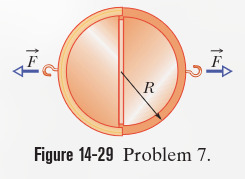
\includegraphics[width=0.45\linewidth]{images/7.jpg}
  \caption{Ilustrasi Pompa Angin nomor 7}
  \label{fig:pompa-angin}
\end{figure}

\diketahui
\begin{align*}
R &= \SI{30}{\centi\metre} = \SI{0,30}{\metre}, &
p_{\text{dalam}} &= \SI{0,10}{\atm}, &
p_{\text{luar}} &= \SI{1,00}{\atm}
\end{align*}

\ditanya\ (a) Pembuktian $F = \pi R^2 \Delta p$; (b) $F$; (c) penjelasan konseptual.

\konsep\ Tekanan fluida bekerja tegak lurus permukaan. Gaya yang menahan kedua belahan
adalah komponen sejajar sumbu tarik dari seluruh gaya tekanan neto $\Delta p$ pada
permukaan satu belahan bola.

\penyelesaian

\textbf{(a)} Ambil sumbu $z$ sepanjang arah gaya tarik. Pada satu belahan bola, tinjau
cincin tipis pada sudut polar $\theta$ (diukur dari sumbu $z$) dengan lebar $R\,d\theta$
dan keliling $2\pi R\sin\theta$. Luas cincin:
\begin{equation}
dA = 2\pi R^2 \sin\theta \, d\theta
\end{equation}
Gaya tekanan neto pada cincin sebesar $\Delta p\,dA$ tegak lurus permukaan; hanya
komponen sejajar sumbu $z$ yang tidak saling meniadakan (komponen radial saling
menghapus oleh simetri). Komponen tersebut adalah $\Delta p\,\cos\theta\,dA$, sehingga
\begin{align}
F &= \int_{0}^{\pi/2} \Delta p \cos\theta \,\left(2\pi R^2 \sin\theta\right) d\theta
   = 2\pi R^2 \Delta p \int_{0}^{\pi/2} \sin\theta\cos\theta \, d\theta \\
  &= 2\pi R^2 \Delta p \left[\tfrac{1}{2}\sin^2\theta\right]_{0}^{\pi/2}
   = \pi R^2 \,\Delta p \qquad \blacksquare
\end{align}
Dengan kata lain, gaya sama dengan $\Delta p$ dikalikan luas proyeksi belahan bola, yaitu
sebuah lingkaran berjari-jari $R$.

\textbf{(b)} Selisih tekanan:
\begin{equation}
\Delta p = (\num{1,00} - \num{0,10})\,\si{\atm} = \SI{0,90}{\atm}
 = (\num{0,90})(\SI{1,013e5}{\pascal}) = \SI{9,12e4}{\pascal}
\end{equation}
Gaya:
\begin{align}
F &= \pi R^2 \,\Delta p = \pi\,(\SI{0,30}{\metre})^2\,(\SI{9,12e4}{\pascal}) \\
  &= (\SI{0,283}{\metre\squared})(\SI{9,12e4}{\pascal}) = \SI{2,58e4}{\newton}
\end{align}

\textbf{(c)} Setiap belahan bola harus ditahan dengan gaya $F$ agar tidak terlepas.
Bila belahan bola yang satu dikaitkan pada dinding yang kokoh, dinding tersebut
memberikan gaya reaksi sebesar $F$ pada belahan itu (hukum III Newton), persis seperti
yang semula diberikan oleh tim kuda di sisi lain. Jadi satu tim kuda yang menarik dengan
gaya $F$ menghasilkan kondisi yang identik, dan tidak diperlukan tim kedua.

\begin{jawaban}
(a) $F = \pi R^2 \,\Delta p$ (terbukti).\\
(b) $F \approx \SI{2,6e4}{\newton}$.\\
(c) Dinding kokoh memberi gaya reaksi $F$ yang sama besar dengan tarikan tim kuda kedua.
\end{jawaban}

% =====================================================
\section*{Soal 8}
\textit{Penyakit dekompresi (the bends) saat penerbangan.} Seorang penyelam dianjurkan
tidak terbang dalam 24 jam setelah menyelam. Hitung perubahan tekanan yang dialami
seorang prajurit pasukan khusus yang menyelam pada kedalaman $\SI{20}{\metre}$ di air
laut pada suatu hari, lalu terjun payung dari ketinggian $\SI{7,6}{\kilo\metre}$
keesokan harinya. Anggap massa jenis udara rata-rata pada rentang ketinggian tersebut
$\SI{0,87}{\kilo\gram\per\metre\cubed}$.

\diketahui
\begin{align*}
h_1 &= \SI{20}{\metre} \ \text{(kedalaman, air laut)}, &
\rho_{\text{laut}} &= \SI{1024}{\kilo\gram\per\metre\cubed}\ \text{(asumsi, nilai standar air laut)}\\
h_2 &= \SI{7,6}{\kilo\metre} = \SI{7,6e3}{\metre}, &
\rho_{\text{udara}} &= \SI{0,87}{\kilo\gram\per\metre\cubed}
\end{align*}

\ditanya\ Perubahan tekanan $\Delta p$ dari kedalaman $\SI{20}{\metre}$ ke ketinggian
$\SI{7,6}{\kilo\metre}$.

\konsep\ Tekanan hidrostatik: $p = p_0 \pm \rho g h$.
Di dalam laut tekanan \emph{bertambah} terhadap $p_0$ (tekanan di permukaan); di
atmosfer pada ketinggian $h_2$ tekanan \emph{berkurang} terhadap $p_0$.
Tekanan permukaan $p_0$ dianggap sama pada kedua hari.

\penyelesaian
\begin{align}
p_1 &= p_0 + \rho_{\text{laut}}\, g\, h_1
 = p_0 + (\num{1024})(\num{9,8})(\num{20}) = p_0 + \SI{2,01e5}{\pascal} \\
p_2 &= p_0 - \rho_{\text{udara}}\, g\, h_2
 = p_0 - (\num{0,87})(\num{9,8})(\num{7,6e3}) = p_0 - \SI{6,48e4}{\pascal}
\end{align}
Perubahan tekanan:
\begin{align}
\Delta p &= p_2 - p_1 = -\left(\rho_{\text{laut}}\, g\, h_1 + \rho_{\text{udara}}\, g\, h_2\right) \\
 &= -\left(\SI{2,01e5}{\pascal} + \SI{6,48e4}{\pascal}\right) = -\SI{2,66e5}{\pascal}
\end{align}

\begin{jawaban}
$\Delta p \approx -\SI{2,7e5}{\pascal}$, yaitu tekanan \emph{turun} sekitar
$\SI{2,7e5}{\pascal}$ ($\approx \SI{2,6}{\atm}$).
\end{jawaban}

% =====================================================
\section*{Soal 9}
\textit{Tekanan darah pada Argentinosaurus.} (a) Sauropoda raksasa berleher panjang ini
memiliki tinggi kepala $\SI{21}{\metre}$ dan tinggi jantung $\SI{9,0}{\metre}$. Berapa
tekanan gauge (hidrostatik) darah di jantung agar tekanan darah di otak
$\SI{80}{\Torr}$ (cukup untuk mengalirkan darah ke otak)? Massa jenis darah
$\SI{1,06e3}{\kilo\gram\per\metre\cubed}$.
(b) Berapa tekanan darah (dalam torr atau mmHg) di kaki?

\diketahui
\begin{align*}
h_{\text{kepala}} &= \SI{21}{\metre}, &
h_{\text{jantung}} &= \SI{9,0}{\metre}, &
h_{\text{kaki}} &= \SI{0}{\metre}\\
p_{\text{otak}} &= \SI{80}{\Torr}, &
\rho &= \SI{1,06e3}{\kilo\gram\per\metre\cubed}
\end{align*}

\ditanya\ (a) $p_{\text{jantung}}$; (b) $p_{\text{kaki}}$.

\konsep\ Beda tekanan dalam fluida statis: $p_{\text{bawah}} = p_{\text{atas}} + \rho g\,\Delta h$.
Konversi: $\SI{1}{\Torr} = \SI{133,3}{\pascal}$.

\penyelesaian

\textbf{(a)} Beda tinggi jantung--otak: $\Delta h_1 = \SI{21}{\metre} - \SI{9,0}{\metre} = \SI{12}{\metre}$.
\begin{align}
\rho g \Delta h_1 &= (\num{1,06e3})(\num{9,8})(\num{12}) = \SI{1,25e5}{\pascal}
 = \frac{\SI{1,25e5}{\pascal}}{\SI{133,3}{\pascal\per\Torr}} = \SI{935}{\Torr} \\
p_{\text{jantung}} &= p_{\text{otak}} + \rho g \Delta h_1
 = \SI{80}{\Torr} + \SI{935}{\Torr} = \SI{1,0e3}{\Torr}
\end{align}

\textbf{(b)} Beda tinggi kaki--jantung: $\Delta h_2 = \SI{9,0}{\metre}$.
\begin{align}
\rho g \Delta h_2 &= (\num{1,06e3})(\num{9,8})(\num{9,0}) = \SI{9,35e4}{\pascal}
 = \SI{701}{\Torr} \\
p_{\text{kaki}} &= p_{\text{jantung}} + \rho g \Delta h_2
 = \SI{1015}{\Torr} + \SI{701}{\Torr} \approx \SI{1,7e3}{\Torr}
\end{align}

\begin{jawaban}
(a) $p_{\text{jantung}} \approx \SI{1,0e3}{\Torr}$ ($\approx \SI{1,3e5}{\pascal}$).\\
(b) $p_{\text{kaki}} \approx \SI{1,7e3}{\Torr}$ ($\approx \SI{1,7e3}{\mmHgunit}$, atau $\approx \SI{2,3e5}{\pascal}$).
\end{jawaban}

% =====================================================
\section*{Soal 10}
Tabung plastik pada Gambar 2 berbentuk U dengan luas penampang
$A = \SI{5,00}{\centi\metre\squared}$. Tabung diisi air hingga lengan pendek
(panjang $d = \SI{0,800}{\metre}$) penuh. Lengan pendek lalu ditutup rapat (disegel),
kemudian air dituangkan perlahan ke lengan panjang. Segel akan lepas jika gaya padanya
melebihi $\SI{9,80}{\newton}$. Berapa tinggi total air di lengan panjang saat segel tepat
akan lepas?

\begin{figure}[H]
  \centering
  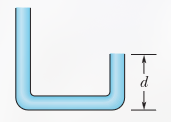
\includegraphics[width=0.45\linewidth]{images/10.png}
  \caption{Ilustrasi Pipa Air nomor 10}
  \label{fig:tangki-L}
\end{figure}

\diketahui
\begin{align*}
A &= \SI{5,00}{\centi\metre\squared} = \SI{5,00e-4}{\metre\squared}, &
d &= \SI{0,800}{\metre}\\
F_{\text{maks}} &= \SI{9,80}{\newton}, &
\rho &= \SI{1,00e3}{\kilo\gram\per\metre\cubed}
\end{align*}

\ditanya\ Tinggi total air di lengan panjang, $h$ (diukur dari dasar tabung).

\konsep\ Lengan panjang terbuka ke atmosfer, sehingga tekanan di dasar tabung
$p_{\text{dasar}} = p_0 + \rho g h$. Pada lengan pendek, titik di bawah segel berada
setinggi $d$ di atas dasar, sehingga tekanan pada segel
\begin{equation*}
p_{\text{segel}} = p_{\text{dasar}} - \rho g d = p_0 + \rho g (h - d)
\end{equation*}
Tekanan atmosfer $p_0$ juga bekerja pada sisi luar segel dan saling meniadakan, sehingga
gaya neto pada segel berasal dari tekanan gauge $\rho g (h-d)$:
\begin{equation*}
F = \rho g (h - d)\, A
\end{equation*}

\penyelesaian
\begin{align}
h - d &= \frac{F_{\text{maks}}}{\rho g A}
 = \frac{\SI{9,80}{\newton}}{(\SI{1,00e3}{\kilo\gram\per\metre\cubed})(\SI{9,8}{\meter\per\second\squared})(\SI{5,00e-4}{\metre\squared})}
 = \SI{2,00}{\metre} \\
h &= d + \SI{2,00}{\metre} = \SI{0,800}{\metre} + \SI{2,00}{\metre} = \SI{2,80}{\metre}
\end{align}

\begin{jawaban}
$h = \SI{2,80}{\metre}$ (diukur dari dasar tabung).
\end{jawaban}

\section*{Soal 11}
\textit{Jerapah menunduk untuk minum.} Kepala seekor jerapah berada $\SI{2,0}{\metre}$ di
atas jantungnya, dan jantungnya $\SI{2,0}{\metre}$ di atas kakinya. Tekanan gauge
(hidrostatik) darah di jantung adalah $\SI{250}{\Torr}$. Anggap jerapah berdiri tegak dan
massa jenis darah $\SI{1,06e3}{\kilo\gram\per\metre\cubed}$. Tentukan tekanan gauge darah
(a) di otak, (b) di kaki, dan (c) pertambahan tekanan darah di otak bila jerapah menurunkan
kepalanya untuk minum dari kolam tanpa merenggangkan kaki dan bergerak perlahan.
 
\diketahui
\begin{align*}
h_{\text{kepala--jantung}} &= \SI{2,0}{\metre}, &
h_{\text{jantung--kaki}} &= \SI{2,0}{\metre}\\
p_{\text{jantung}} &= \SI{250}{\Torr}, &
\rho &= \SI{1,06e3}{\kilo\gram\per\metre\cubed}
\end{align*}
 
\ditanya\ (a) $p_{\text{otak}}$; (b) $p_{\text{kaki}}$; (c) $\Delta p_{\text{otak}}$ saat kepala diturunkan.
 
\konsep\ Pada fluida statis, $p_{\text{bawah}} = p_{\text{atas}} + \rho g\,\Delta h$.
Tekanan darah di jantung dianggap tetap pada (c).
 
\penyelesaian
 
Beda tekanan untuk selisih tinggi $\SI{2,0}{\metre}$:
\begin{equation}
\rho g h = (\num{1,06e3})(\num{9,8})(\num{2,0}) = \SI{2,08e4}{\pascal}
 = \frac{\SI{2,08e4}{\pascal}}{\SI{133,3}{\pascal\per\Torr}} = \SI{156}{\Torr}
\end{equation}
 
\textbf{(a)} Otak berada di atas jantung, sehingga tekanannya lebih kecil:
\begin{equation}
p_{\text{otak}} = p_{\text{jantung}} - \rho g h = \SI{250}{\Torr} - \SI{156}{\Torr} = \SI{94}{\Torr}
\end{equation}
 
\textbf{(b)} Kaki berada di bawah jantung, sehingga tekanannya lebih besar:
\begin{equation}
p_{\text{kaki}} = p_{\text{jantung}} + \rho g h = \SI{250}{\Torr} + \SI{156}{\Torr} \approx \SI{4,1e2}{\Torr}
\end{equation}
 
\textbf{(c)} Saat minum, kepala berada setinggi kaki, yaitu $\SI{2,0}{\metre}$ di bawah
jantung. Tekanan di otak menjadi $p_{\text{jantung}} + \rho g h = \SI{406}{\Torr}$, sehingga
pertambahannya
\begin{equation}
\Delta p_{\text{otak}} = \SI{406}{\Torr} - \SI{94}{\Torr} = \SI{312}{\Torr}
 \quad \left(= \rho g\,(\SI{4,0}{\metre})\right)
\end{equation}
 
\begin{jawaban}
(a) $p_{\text{otak}} \approx \SI{94}{\Torr}$.\\
(b) $p_{\text{kaki}} \approx \SI{4,1e2}{\Torr}$.\\
(c) $\Delta p_{\text{otak}} \approx \SI{3,1e2}{\Torr}$.
\end{jawaban}
 
% =====================================================
\section*{Soal 12}
Kedalaman maksimum $d_{\max}$ yang dapat dicapai seorang penyelam ber-\textit{snorkel}
ditentukan oleh massa jenis air dan kenyataan bahwa paru-paru manusia hanya dapat
berfungsi melawan beda tekanan maksimum (antara dalam dan luar rongga dada)
sebesar $\SI{0,050}{\atm}$. Berapa selisih $d_{\max}$ di air tawar dan di air Laut Mati
(massa jenis $\SI{1,5e3}{\kilo\gram\per\metre\cubed}$)?
 
\diketahui
\begin{align*}
\Delta p_{\max} &= \SI{0,050}{\atm} = \SI{5,07e3}{\pascal}\\
\rho_{\text{tawar}} &= \SI{1,00e3}{\kilo\gram\per\metre\cubed}, &
\rho_{\text{Laut Mati}} &= \SI{1,5e3}{\kilo\gram\per\metre\cubed}
\end{align*}
 
\ditanya\ $d_{\max,\text{tawar}} - d_{\max,\text{LM}}$.
 
\konsep\ Beda tekanan akibat kedalaman: $\Delta p = \rho g\, d$, sehingga
$d_{\max} = \Delta p_{\max}/(\rho g)$.
 
\penyelesaian
\begin{align}
d_{\max,\text{tawar}} &= \frac{\SI{5,07e3}{\pascal}}{(\num{1,00e3})(\num{9,8})} = \SI{0,517}{\metre} \\
d_{\max,\text{LM}} &= \frac{\SI{5,07e3}{\pascal}}{(\num{1,5e3})(\num{9,8})} = \SI{0,345}{\metre} \\
\Delta d &= \SI{0,517}{\metre} - \SI{0,345}{\metre} = \SI{0,172}{\metre}
\end{align}
 
\begin{jawaban}
$\Delta d_{\max} \approx \SI{0,17}{\metre}$ (kedalaman maksimum di air tawar lebih besar
sekitar $\SI{17}{\centi\metre}$ daripada di Laut Mati).
\end{jawaban}
 
% =====================================================
\section*{Soal 13}
Pada kedalaman $\SI{10,9}{\kilo\metre}$, Challenger Deep di Palung Mariana adalah titik
terdalam di semua samudra. Pada tahun 1960, Donald Walsh dan Jacques Piccard mencapainya
dengan batiskaf \textit{Trieste}. Anggap massa jenis air laut seragam,
$\SI{1024}{\kilo\gram\per\metre\cubed}$. Perkirakan tekanan hidrostatik (dalam atmosfer)
yang harus ditahan \textit{Trieste}.
 
\diketahui
\begin{align*}
h &= \SI{10,9}{\kilo\metre} = \SI{1,09e4}{\metre}, &
\rho &= \SI{1024}{\kilo\gram\per\metre\cubed}
\end{align*}
 
\ditanya\ Tekanan hidrostatik $p$ dalam atm.
 
\konsep\ $p = \rho g h$ (tekanan atmosfer di permukaan, $\approx \SI{1}{\atm}$, dapat
diabaikan terhadap hasil yang sangat besar ini).
 
\penyelesaian
\begin{align}
p &= \rho g h = (\num{1024})(\num{9,8})(\num{1,09e4}) = \SI{1,09e8}{\pascal} \\
  &= \frac{\SI{1,09e8}{\pascal}}{\SI{1,013e5}{\pascal\per\atm}} = \SI{1,08e3}{\atm}
\end{align}
 
\begin{jawaban}
$p \approx \SI{1,08e3}{\atm}$ ($\approx \SI{1,09e8}{\pascal}$).
\end{jawaban}
 
% =====================================================
\section*{Soal 14}
Hitung selisih tekanan darah hidrostatik antara otak dan kaki seseorang yang tingginya
$\SI{1,83}{\metre}$. Massa jenis darah $\SI{1,06e3}{\kilo\gram\per\metre\cubed}$.
 
\diketahui
\begin{align*}
h &= \SI{1,83}{\metre}, &
\rho &= \SI{1,06e3}{\kilo\gram\per\metre\cubed}
\end{align*}
 
\ditanya\ $\Delta p$ antara kaki dan otak.
 
\konsep\ Orang berdiri tegak sehingga beda tinggi otak--kaki sama dengan tinggi badan:
$\Delta p = \rho g h$.
 
\penyelesaian
\begin{align}
\Delta p &= (\num{1,06e3})(\num{9,8})(\num{1,83}) = \SI{1,90e4}{\pascal}
 \ \left(\approx \SI{143}{\Torr}\right)
\end{align}
 
\begin{jawaban}
$\Delta p \approx \SI{1,90e4}{\pascal}$ (tekanan di kaki lebih besar daripada di otak).
\end{jawaban}
 
% =====================================================
\section*{Soal 15}
Berapa tekanan gauge yang harus dihasilkan sebuah mesin agar dapat menyedot lumpur
bermassa jenis $\SI{1800}{\kilo\gram\per\metre\cubed}$ naik melalui sebuah pipa setinggi
$\SI{1,5}{\metre}$?
 
\diketahui
\begin{align*}
\rho &= \SI{1800}{\kilo\gram\per\metre\cubed}, &
h &= \SI{1,5}{\metre}
\end{align*}
 
\ditanya\ Tekanan gauge $p_g$ yang dihasilkan mesin.
 
\konsep\ Lumpur naik karena tekanan di atas kolom (di mesin) lebih rendah daripada tekanan
atmosfer di permukaan lumpur. Agar kolom setinggi $h$ tertahan,
$p_0 - p = \rho g h$, sehingga tekanan gauge $p_g = p - p_0 = -\rho g h$
(negatif, yaitu hisapan).
 
\penyelesaian
\begin{align}
\left|p_g\right| &= \rho g h = (\num{1800})(\num{9,8})(\num{1,5}) = \SI{2,6e4}{\pascal}
 \ \left(\approx \SI{0,26}{\atm}\right)
\end{align}
 
\begin{jawaban}
$p_g \approx -\SI{2,6e4}{\pascal}$ (di bawah tekanan atmosfer); besar hisapan
$\SI{2,6e4}{\pascal}$.
\end{jawaban}

\section*{Soal 16}
\textit{Snorkeling oleh manusia dan gajah.} Ketika seseorang ber-\textit{snorkel}, paru-parunya
terhubung langsung ke atmosfer melalui tabung snorkel sehingga bertekanan atmosfer.
Berapa selisih (dalam atmosfer) antara tekanan udara dalam paru-paru dan tekanan air pada
tubuh bila panjang tabung snorkel (a) $\SI{20}{\centi\metre}$ (keadaan standar) dan
(b) $\SI{4,0}{\metre}$ (kemungkinan fatal)?
 
\diketahui
\begin{align*}
h_a &= \SI{20}{\centi\metre} = \SI{0,20}{\metre}, &
h_b &= \SI{4,0}{\metre}, &
\rho &= \SI{1,00e3}{\kilo\gram\per\metre\cubed}
\end{align*}
 
\ditanya\ $\Delta p_a$ dan $\Delta p_b$ dalam atm.
 
\konsep\ Paru-paru bertekanan $p_0$ (atmosfer), sedangkan tekanan air pada tubuh pada
kedalaman $h$ adalah $p_0 + \rho g h$. Jadi selisihnya
$\Delta p = \rho g h$.
 
\penyelesaian
 
\textbf{(a)}
\begin{align}
\Delta p_a &= (\num{1,00e3})(\num{9,8})(\num{0,20}) = \SI{1,96e3}{\pascal}
 = \frac{\SI{1,96e3}{\pascal}}{\SI{1,013e5}{\pascal\per\atm}} = \SI{1,9e-2}{\atm}
\end{align}
 
\textbf{(b)}
\begin{align}
\Delta p_b &= (\num{1,00e3})(\num{9,8})(\num{4,0}) = \SI{3,92e4}{\pascal}
 = \frac{\SI{3,92e4}{\pascal}}{\SI{1,013e5}{\pascal\per\atm}} = \SI{0,39}{\atm}
\end{align}
 
\begin{jawaban}
(a) $\Delta p \approx \SI{0,019}{\atm}$.\\
(b) $\Delta p \approx \SI{0,39}{\atm}$.
\end{jawaban}
 
% =====================================================
\section*{Soal 17}
Awak kapal berusaha menyelamatkan diri dari kapal selam yang rusak pada kedalaman
$\SI{100}{\metre}$ di bawah permukaan. Berapa gaya yang harus dikerahkan pada sebuah
palka (\textit{hatch}) berukuran $\SI{1,2}{\metre} \times \SI{0,60}{\metre}$ agar
palka terdorong keluar pada kedalaman tersebut? Anggap massa jenis air laut
$\SI{1024}{\kilo\gram\per\metre\cubed}$ dan tekanan udara di dalam kapal selam
$\SI{1,00}{\atm}$.
 
\diketahui
\begin{align*}
h &= \SI{100}{\metre}, &
A &= (\SI{1,2}{\metre})(\SI{0,60}{\metre}) = \SI{0,72}{\metre\squared}\\
\rho &= \SI{1024}{\kilo\gram\per\metre\cubed}, &
p_{\text{dalam}} &= p_0 = \SI{1,00}{\atm}
\end{align*}
 
\ditanya\ Gaya minimum $F$ untuk mendorong palka keluar.
 
\konsep\ Tekanan di luar palka $p_{\text{luar}} = p_0 + \rho g h$, sedangkan di dalam $p_0$.
Gaya neto yang menekan palka ke dalam berasal dari tekanan gauge $\rho g h$. Gaya dorong
yang diperlukan paling sedikit sebesar gaya ini:
\begin{equation*}
F = (p_{\text{luar}} - p_{\text{dalam}})\,A = \rho g h A
\end{equation*}
 
\penyelesaian
\begin{align}
\rho g h &= (\num{1024})(\num{9,8})(\num{100}) = \SI{1,00e6}{\pascal} \\
F &= (\SI{1,00e6}{\pascal})(\SI{0,72}{\metre\squared}) = \SI{7,2e5}{\newton}
\end{align}
 
\begin{jawaban}
$F \approx \SI{7,2e5}{\newton}$.
\end{jawaban}
 
% =====================================================
\section*{Soal 18}
Pada Gambar 3, sebuah tabung terbuka dengan panjang $L = \SI{1,8}{\metre}$ dan luas
penampang $A = \SI{4,6}{\centi\metre\squared}$ dipasang tegak di atas sebuah drum silinder
berdiameter $D = \SI{1,2}{\metre}$ dan tinggi $H = \SI{1,8}{\metre}$. Drum dan tabung diisi
air hingga puncak tabung. Hitung perbandingan antara gaya hidrostatik pada dasar drum dan
gaya gravitasi pada air di dalam drum. Mengapa perbandingan itu tidak sama dengan $1{,}0$?
(Abaikan tekanan atmosfer.)

\begin{figure}[H]
  \centering
  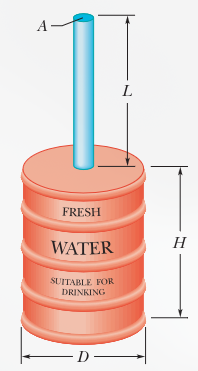
\includegraphics[width=0.45\linewidth]{images/18.png}
  \caption{Ilustrasi Tangki dan Silinder Tangki nomor 18}
  \label{fig:barrel}
\end{figure}
 
\diketahui
\begin{align*}
L &= \SI{1,8}{\metre}, &
A &= \SI{4,6e-4}{\metre\squared}\\
D &= \SI{1,2}{\metre}, &
H &= \SI{1,8}{\metre}
\end{align*}
 
\ditanya\ Rasio $F_{\text{dasar}}/W_{\text{drum}}$ dan penjelasannya.
 
\konsep\ Tekanan gauge di dasar drum ditentukan oleh \emph{kedalaman total} air di atasnya
(drum ditambah tabung): $p = \rho g (H + L)$. Luas dasar drum $A_d = \pi D^2/4$.
 
\penyelesaian
 
Luas dasar drum:
\begin{equation}
A_d = \frac{\pi D^2}{4} = \frac{\pi (\SI{1,2}{\metre})^2}{4} = \SI{1,13}{\metre\squared}
\end{equation}
Gaya hidrostatik pada dasar drum:
\begin{equation}
F_{\text{dasar}} = \rho g (H+L) A_d
 = (\num{1,00e3})(\num{9,8})(\num{3,6})(\num{1,13}) = \SI{3,99e4}{\newton}
\end{equation}
Berat air di dalam drum (volume drum $= A_d H$; berat air dalam tabung hanya
$\rho g L A \approx \SI{8}{\newton}$ sehingga dapat diabaikan):
\begin{equation}
W_{\text{drum}} = \rho g H A_d = (\num{1,00e3})(\num{9,8})(\num{1,8})(\num{1,13}) = \SI{1,99e4}{\newton}
\end{equation}
Perbandingan:
\begin{equation}
\frac{F_{\text{dasar}}}{W_{\text{drum}}} = \frac{\rho g (H+L) A_d}{\rho g H A_d}
 = \frac{H + L}{H} = \frac{\SI{3,6}{\metre}}{\SI{1,8}{\metre}} = 2{,}0
\end{equation}
 
\textbf{Penjelasan:} Gaya pada dasar drum bergantung pada tekanan, yaitu pada kedalaman
total air ($H + L$), bukan pada berat air di dalam drum. Air di dalam tabung menekan air
di drum, dan tekanan ini diteruskan ke seluruh fluida (prinsip Pascal). Akibatnya, tutup
drum mendorong air ke bawah dengan gaya $\rho g L (A_d - A) $ ke bawah, selain berat air
itu sendiri, sehingga dasar drum menopang lebih dari berat air dalam drum.
(Fenomena ini dikenal sebagai \textit{paradoks hidrostatik}.)
 
\begin{jawaban}
$F_{\text{dasar}}/W_{\text{drum}} \approx \num{2,0}$ (dengan $F_{\text{dasar}} \approx \SI{4,0e4}{\newton}$
dan $W_{\text{drum}} \approx \SI{2,0e4}{\newton}$). Rasio tidak sama dengan $1{,}0$ karena
tutup drum memberi gaya ke bawah pada air akibat tekanan dari kolom air di tabung.
\end{jawaban}
 
% =====================================================
\section*{Soal 19}
Sebuah akuarium besar setinggi $\SI{5,00}{\metre}$ diisi air tawar hingga kedalaman
$\SI{2,00}{\metre}$. Salah satu dindingnya terbuat dari plastik tebal selebar
$\SI{8,00}{\metre}$. Berapa pertambahan gaya total pada dinding tersebut bila akuarium
kemudian diisi hingga kedalaman $\SI{4,00}{\metre}$?
 
\diketahui
\begin{align*}
w &= \SI{8,00}{\metre}, &
h_1 &= \SI{2,00}{\metre}, &
h_2 &= \SI{4,00}{\metre}, &
\rho &= \SI{1,00e3}{\kilo\gram\per\metre\cubed}
\end{align*}
 
\ditanya\ $\Delta F = F_2 - F_1$.
 
\konsep\ Tekanan gauge bertambah linear terhadap kedalaman $y$: $p = \rho g y$. Gaya pada
dinding diperoleh dengan mengintegralkan tekanan pada luas dinding yang terendam
($dA = w\,dy$); tekanan atmosfer bekerja pada kedua sisi dinding sehingga saling
meniadakan.
\begin{equation*}
F = \int_{0}^{h} \rho g y \, w\, dy = \tfrac{1}{2}\rho g w h^2
\end{equation*}
 
\penyelesaian
\begin{align}
F_1 &= \tfrac{1}{2}(\num{1,00e3})(\num{9,8})(\num{8,00})(\num{2,00})^2 = \SI{1,57e5}{\newton} \\
F_2 &= \tfrac{1}{2}(\num{1,00e3})(\num{9,8})(\num{8,00})(\num{4,00})^2 = \SI{6,27e5}{\newton} \\
\Delta F &= F_2 - F_1 = \tfrac{1}{2}\rho g w \left(h_2^2 - h_1^2\right) = \SI{4,70e5}{\newton}
\end{align}
 
\begin{jawaban}
$\Delta F \approx \SI{4,70e5}{\newton}$.
\end{jawaban}
 
% =====================================================
\section*{Soal 20}
Tangki ikan berbentuk L pada Gambar 4 diisi air dan terbuka di bagian atas. Bila
$d = \SI{5,0}{\metre}$, berapa gaya total yang dikerjakan air (a) pada permukaan $A$ dan
(b) pada permukaan $B$?

\begin{figure}[H]
  \centering
  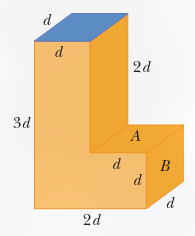
\includegraphics[width=0.45\linewidth]{images/20.png}
  \caption{Ilustrasi Tangki Ikan 'L' nomor 20}
  \label{fig:fish-tank}
\end{figure}
 
\diketahui\ (dari Gambar 4)
\begin{itemize}[nosep]
  \item Kolom tegak: tinggi $3d$, penampang $d \times d$; permukaan air berada di puncaknya.
  \item Kaki tangki: tinggi $d$, panjang tambahan $d$ ke samping, lebar (ke dalam bidang gambar) $d$.
  \item Permukaan $A$: langit-langit horizontal kaki tangki, luas $d \times d$, pada kedalaman $2d$.
  \item Permukaan $B$: sisi ujung vertikal kaki tangki, luas $d \times d$, membentang dari kedalaman $2d$ sampai $3d$.
  \item $d = \SI{5,0}{\metre}$, $\rho = \SI{1,00e3}{\kilo\gram\per\metre\cubed}$.
\end{itemize}
 
\ditanya\ $F_A$ dan $F_B$.
 
\konsep\ Tekanan gauge pada kedalaman $y$ adalah $\rho g y$.
 
\penyelesaian
 
\textbf{(a)} Seluruh permukaan $A$ berada pada kedalaman yang sama, $2d$, sehingga tekanan
seragam:
\begin{align}
F_A &= \rho g (2d)\,(d \cdot d) = 2\rho g d^3 \\
    &= 2(\num{1,00e3})(\num{9,8})(\num{5,0})^3 = \SI{2,45e6}{\newton}
\end{align}
 
\textbf{(b)} Tekanan pada $B$ berubah linear terhadap kedalaman, sehingga gaya dihitung dari
integral (atau dari tekanan rata-rata, yaitu pada kedalaman rata-rata $2{,}5d$):
\begin{align}
F_B &= \int_{2d}^{3d} \rho g y \, d\, dy = \tfrac{1}{2}\rho g d\left[(3d)^2 - (2d)^2\right]
 = \tfrac{5}{2}\rho g d^3 \\
    &= \tfrac{5}{2}(\num{1,00e3})(\num{9,8})(\num{5,0})^3 = \SI{3,06e6}{\newton}
\end{align}
 
\begin{jawaban}
(a) $F_A \approx \SI{2,5e6}{\newton}$ (tepatnya $\SI{2,45e6}{\newton}$), arah ke atas.\\
(b) $F_B \approx \SI{3,1e6}{\newton}$, arah horizontal ke luar.
\end{jawaban}

\section*{Soal 21}
Dua bejana silinder identik dengan dasar pada tingkat yang sama masing-masing berisi cairan
bermassa jenis $\SI{1,30e3}{\kilo\gram\per\metre\cubed}$. Luas tiap dasar $\SI{4,00}{\centi\metre\squared}$,
tetapi tinggi cairan di satu bejana $\SI{0,854}{\metre}$ dan di bejana lain $\SI{1,560}{\metre}$.
Tentukan usaha yang dilakukan gaya gravitasi dalam menyamakan tinggi permukaan ketika
kedua bejana dihubungkan.
 
\diketahui
\begin{align*}
\rho &= \SI{1,30e3}{\kilo\gram\per\metre\cubed}, &
A &= \SI{4,00}{\centi\metre\squared} = \SI{4,00e-4}{\metre\squared}\\
h_1 &= \SI{0,854}{\metre}, &
h_2 &= \SI{1,560}{\metre}
\end{align*}
 
\ditanya\ Usaha gravitasi $W_g$ selama penyamaan tinggi permukaan.
 
\konsep\ Usaha gravitasi sama dengan penurunan energi potensial:
$W_g = U_{\text{awal}} - U_{\text{akhir}}$. Untuk kolom cairan setinggi $h$ dan luas $A$,
massa $m = \rho A h$ dan pusat massanya berada pada $h/2$, sehingga
$U = \tfrac{1}{2}\rho g A h^2$. Volume cairan tetap, jadi tinggi akhir di kedua bejana
$h_f = (h_1 + h_2)/2$.
 
\penyelesaian
\begin{align}
U_{\text{awal}} &= \tfrac{1}{2}\rho g A \left(h_1^2 + h_2^2\right), &
U_{\text{akhir}} &= \tfrac{1}{2}\rho g A \,(2 h_f^2) = \tfrac{1}{4}\rho g A\,(h_1 + h_2)^2
\end{align}
\begin{align}
W_g &= U_{\text{awal}} - U_{\text{akhir}}
 = \tfrac{1}{4}\rho g A\,(h_1 - h_2)^2 \\
 &= \tfrac{1}{4}(\num{1,30e3})(\num{9,8})(\num{4,00e-4})(\num{0,854} - \num{1,560})^2 \\
 &= \tfrac{1}{4}(\SI{5,10}{\newton\per\metre})(\SI{0,498}{\metre\squared})
  = \SI{0,635}{\joule}
\end{align}
 
\begin{jawaban}
$W_g \approx \SI{0,635}{\joule}$.
\end{jawaban}
 
% =====================================================
\section*{Soal 22}
\textit{g-LOC pada pertempuran udara.} Saat pilot pesawat tempur melakukan manuver belok
tajam pada kecepatan tinggi, tekanan darah di otak turun sehingga darah tidak lagi mengalir
ke otak. Jika jantung mempertahankan tekanan gauge (hidrostatik) di aorta sebesar
$\SI{120}{\Torr}$ ketika pilot mengalami percepatan sentripetal horizontal $4g$, berapa
tekanan darah (dalam torr) di otak yang berada $\SI{30}{\centi\metre}$ ke arah dalam
(menuju pusat lintasan) dari jantung? Massa jenis darah $\SI{1,06e3}{\kilo\gram\per\metre\cubed}$.
 
\diketahui
\begin{align*}
p_{\text{jantung}} &= \SI{120}{\Torr}, &
a &= 4g = \SI{39,2}{\meter\per\second\squared}, &
\Delta r &= \SI{0,30}{\metre}, &
\rho &= \SI{1,06e3}{\kilo\gram\per\metre\cubed}
\end{align*}
 
\ditanya\ $p_{\text{otak}}$ dalam torr.
 
\konsep\ Dalam kerangka pilot yang berakselerasi sentripetal $a = 4g$, fluida seolah berada
dalam medan gravitasi efektif sebesar $4g$ yang mengarah \emph{keluar} (menjauhi pusat
belokan). Otak berada $\SI{30}{\centi\metre}$ ``di atas'' jantung terhadap medan efektif
tersebut, sehingga tekanannya lebih kecil:
$p_{\text{otak}} = p_{\text{jantung}} - \rho\,(4g)\,\Delta r$.
 
\penyelesaian
\begin{align}
\rho\,(4g)\,\Delta r &= (\num{1,06e3})(\num{39,2})(\num{0,30}) = \SI{1,25e4}{\pascal}
 = \frac{\SI{1,25e4}{\pascal}}{\SI{133,32}{\pascal\per\Torr}} = \SI{93,5}{\Torr} \\
p_{\text{otak}} &= \SI{120}{\Torr} - \SI{93,5}{\Torr} = \SI{26,5}{\Torr}
\end{align}
 
\begin{jawaban}
$p_{\text{otak}} \approx \SI{27}{\Torr}$ (tepatnya $\SI{26,5}{\Torr}$), jauh lebih kecil dari tekanan
di jantung sehingga aliran darah ke otak terganggu.
\end{jawaban}
 
% =====================================================
\section*{Soal 23}
Dalam menganalisis ciri-ciri geologis tertentu, sering dianggap bahwa tekanan pada suatu
\textit{tingkat kompensasi} horizontal di dalam Bumi bernilai sama di wilayah yang luas dan
sama dengan tekanan akibat gaya gravitasi pada material di atasnya. Model ini mensyaratkan
bahwa gunung memiliki \textit{akar} batuan benua yang menembus ke dalam mantel yang lebih
rapat (Gambar 5). Untuk gunung setinggi $H = \SI{6,0}{\kilo\metre}$ pada benua setebal
$T = \SI{32}{\kilo\metre}$, dengan batuan benua bermassa jenis $\SI{2,9}{\gram\per\cubic\centi\metre}$
dan mantel $\SI{3,3}{\gram\per\cubic\centi\metre}$, hitung kedalaman $D$ akar gunung.

\begin{figure}[H]
  \centering
  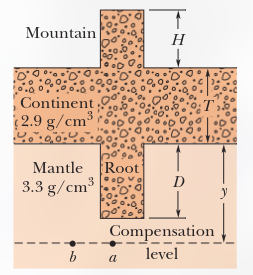
\includegraphics[width=0.45\linewidth]{images/23.png}
  \caption{Ilustrasi Tanah nomor 23}
  \label{fig:land-geography}
\end{figure}
 
\diketahui
\begin{align*}
H &= \SI{6,0}{\kilo\metre}, &
T &= \SI{32}{\kilo\metre}, &
\rho_b &= \SI{2,9}{\gram\per\cubic\centi\metre}, &
\rho_m &= \SI{3,3}{\gram\per\cubic\centi\metre}
\end{align*}
 
\ditanya\ Kedalaman akar $D$.
 
\konsep\ Tekanan pada titik $a$ (di bawah benua biasa) dan titik $b$ (di bawah gunung)
pada tingkat kompensasi harus sama, $p_a = p_b$. Tingkat kompensasi berada pada jarak $y$
di bawah dasar akar.
 
\penyelesaian
 
Kolom di atas titik $b$ (gunung + benua + akar + mantel setebal $y$):
\begin{equation}
p_b = \rho_b g\,(H + T + D) + \rho_m g\, y
\end{equation}
Kolom di atas titik $a$ (benua + mantel setebal $D + y$):
\begin{equation}
p_a = \rho_b g\, T + \rho_m g\,(D + y)
\end{equation}
Menyamakan $p_a = p_b$, suku $y$ dan $T$ saling meniadakan:
\begin{align}
\rho_b\,(H + D) &= \rho_m D \\
D &= \frac{\rho_b H}{\rho_m - \rho_b}
 = \frac{(\num{2,9})(\SI{6,0}{\kilo\metre})}{\num{3,3} - \num{2,9}} = \SI{43,5}{\kilo\metre}
\end{align}
 
\begin{jawaban}
$D \approx \SI{44}{\kilo\metre}$.
\end{jawaban}
 
% =====================================================
\section*{Soal 24}
Pada Gambar 6, air berdiri pada kedalaman $D = \SI{35,0}{\metre}$ di belakang muka hulu
vertikal sebuah bendungan selebar $W = \SI{314}{\metre}$. Tentukan (a) gaya horizontal neto
pada bendungan akibat tekanan gauge air, (b) torsi neto akibat gaya tersebut terhadap garis
horizontal yang melalui titik $O$ (di dasar) dan sejajar lebar bendungan, serta (c) lengan
momen torsi tersebut.

\begin{figure}[H]
  \centering
  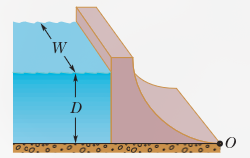
\includegraphics[width=0.45\linewidth]{images/24.png}
  \caption{Gambar 6 Ilustrasi Bendungan nomor 24}
  \label{fig:dam}
\end{figure}
 
\diketahui
\begin{align*}
D &= \SI{35,0}{\metre}, &
W &= \SI{314}{\metre}, &
\rho &= \SI{1,00e3}{\kilo\gram\per\metre\cubed}
\end{align*}
 
\ditanya\ (a) $F$; (b) $\tau$ terhadap $O$; (c) lengan momen $r_{\perp}$.
 
\konsep\ Pada kedalaman $y$ dari permukaan, tekanan gauge $p = \rho g y$. Elemen gaya pada
strip setinggi $dy$ dan lebar $W$: $dF = \rho g y\,W\,dy$. Titik $O$ berada di dasar, sehingga
lengan momen strip tersebut adalah $(D - y)$.
 
\penyelesaian
 
\textbf{(a)}
\begin{align}
F &= \int_{0}^{D} \rho g y\, W\, dy = \tfrac{1}{2}\rho g W D^2 \\
  &= \tfrac{1}{2}(\num{1,00e3})(\num{9,8})(\num{314})(\num{35,0})^2 = \SI{1,88e9}{\newton}
\end{align}
 
\textbf{(b)}
\begin{align}
\tau &= \int_{0}^{D} \rho g y\, W\,(D - y)\, dy
 = \rho g W\left[\frac{D y^2}{2} - \frac{y^3}{3}\right]_{0}^{D} = \frac{\rho g W D^3}{6} \\
 &= \frac{(\num{1,00e3})(\num{9,8})(\num{314})(\num{35,0})^3}{6} = \SI{2,20e10}{\newton\metre}
\end{align}
 
\textbf{(c)}
\begin{equation}
r_{\perp} = \frac{\tau}{F} = \frac{\rho g W D^3/6}{\rho g W D^2/2} = \frac{D}{3}
 = \frac{\SI{35,0}{\metre}}{3} = \SI{11,7}{\metre}
\end{equation}
Jadi gaya neto efektif bekerja pada ketinggian $D/3$ di atas dasar bendungan.
 
\begin{jawaban}
(a) $F \approx \SI{1,88e9}{\newton}$.\\
(b) $\tau \approx \SI{2,20e10}{\newton\metre}$.\\
(c) $r_{\perp} \approx \SI{11,7}{\metre}$ (yaitu $D/3$).
\end{jawaban}
 
% =====================================================
\section*{Soal 25}
Pada suatu pengamatan, tinggi kolom raksa pada barometer raksa (Gambar 7) terukur
$h = \SI{740,35}{\milli\metre}$. Suhu $\SI{-5,0}{\celsius}$, pada suhu itu massa jenis raksa
$\rho = \SI{1,3608e4}{\kilo\gram\per\metre\cubed}$. Percepatan gravitasi di lokasi barometer
$\SI{9,7835}{\meter\per\second\squared}$. Berapa tekanan atmosfer di lokasi tersebut dalam
pascal dan dalam torr?

\begin{figure}[H]
  \centering
  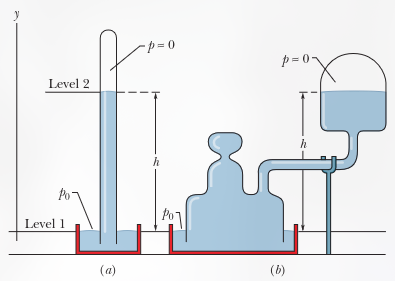
\includegraphics[width=0.45\linewidth]{images/25.png}
  \caption{Ilustrasi Barometer Merkuri nomor 25}
  \label{fig:mercury-barometer}
\end{figure}
 
\diketahui
\begin{align*}
h &= \SI{740,35}{\milli\metre} = \SI{0,74035}{\metre}, &
\rho &= \SI{1,3608e4}{\kilo\gram\per\metre\cubed}, &
g &= \SI{9,7835}{\meter\per\second\squared}
\end{align*}
 
\ditanya\ Tekanan atmosfer $p_0$ dalam Pa dan torr.
 
\konsep\ Pada barometer raksa, tekanan atmosfer sama dengan tekanan hidrostatik kolom raksa:
$p_0 = \rho g h$. Konversi: $\SI{1}{\Torr} = \SI{133,322}{\pascal}$.
 
\penyelesaian
\begin{align}
p_0 &= \rho g h = (\num{1,3608e4})(\num{9,7835})(\num{0,74035}) = \SI{9,857e4}{\pascal} \\
 &= \frac{\SI{9,857e4}{\pascal}}{\SI{133,322}{\pascal\per\Torr}} = \SI{739,3}{\Torr}
\end{align}
 
\begin{jawaban}
$p_0 \approx \SI{9,86e4}{\pascal} \approx \SI{739}{\Torr}$.
\end{jawaban}

\section*{Soal 26}
Untuk menyedot limun bermassa jenis $\SI{1000}{\kilo\gram\per\metre\cubed}$ naik melalui
sedotan hingga ketinggian maksimum $\SI{4,0}{\centi\metre}$, berapa tekanan gauge minimum
(dalam atmosfer) yang harus Anda hasilkan di dalam paru-paru?
 
\diketahui
\begin{align*}
\rho &= \SI{1000}{\kilo\gram\per\metre\cubed}, &
h &= \SI{4,0}{\centi\metre} = \SI{4,0e-2}{\metre}
\end{align*}
 
\ditanya\ Tekanan gauge minimum $p_g$ dalam atm.
 
\konsep\ Limun naik karena tekanan di dalam mulut lebih rendah daripada tekanan atmosfer di
permukaan limun. Agar kolom setinggi $h$ tertahan, $p_0 - p = \rho g h$, sehingga tekanan
gauge $p_g = p - p_0 = -\rho g h$ (negatif, berarti di bawah tekanan atmosfer).
 
\penyelesaian
\begin{align}
\left|p_g\right| &= \rho g h = (\num{1000})(\num{9,8})(\num{4,0e-2}) = \SI{3,9e2}{\pascal} \\
 &= \frac{\SI{3,9e2}{\pascal}}{\SI{1,013e5}{\pascal\per\atm}} = \SI{3,9e-3}{\atm}
\end{align}
 
\begin{jawaban}
$p_g \approx -\SI{3,9e-3}{\atm}$ (hisapan; besarnya $\SI{3,9e-3}{\atm}$ di bawah tekanan atmosfer).
\end{jawaban}
 
% =====================================================
\section*{Soal 27}
Berapa tinggi atmosfer bila massa jenis udara (a) seragam dan (b) berkurang secara linear
hingga nol terhadap ketinggian? Anggap tekanan di permukaan laut $\SI{1,0}{\atm}$ dan massa
jenis udara di permukaan laut $\SI{1,3}{\kilo\gram\per\metre\cubed}$.
 
\diketahui
\begin{align*}
p_0 &= \SI{1,0}{\atm} = \SI{1,013e5}{\pascal}, &
\rho_0 &= \SI{1,3}{\kilo\gram\per\metre\cubed}
\end{align*}
 
\ditanya\ Tinggi atmosfer $h$ untuk kedua model massa jenis.
 
\konsep\ Tekanan di permukaan laut sama dengan berat kolom udara per satuan luas di
atasnya: $p_0 = \int_{0}^{h} \rho(y)\, g\, dy$.
 
\penyelesaian
 
\textbf{(a) Massa jenis seragam:} $\rho(y) = \rho_0$.
\begin{align}
p_0 &= \rho_0 g h \\
h &= \frac{p_0}{\rho_0 g} = \frac{\SI{1,013e5}{\pascal}}{(\SI{1,3}{\kilo\gram\per\metre\cubed})(\SI{9,8}{\meter\per\second\squared})}
 = \SI{7,95e3}{\metre}
\end{align}
 
\textbf{(b) Massa jenis berkurang linear menjadi nol di $y = h$:}
$\rho(y) = \rho_0\left(1 - y/h\right)$.
\begin{align}
p_0 &= \int_{0}^{h} \rho_0 \left(1 - \frac{y}{h}\right) g \, dy
 = \rho_0 g \left[y - \frac{y^2}{2h}\right]_{0}^{h} = \frac{\rho_0 g h}{2} \\
h &= \frac{2 p_0}{\rho_0 g} = 2\,(\SI{7,95e3}{\metre}) = \SI{1,59e4}{\metre}
\end{align}
 
\begin{jawaban}
(a) $h \approx \SI{8,0}{\kilo\metre}$.\\
(b) $h \approx \SI{16}{\kilo\metre}$.
\end{jawaban}
 
% =====================================================
\section*{Soal 28}
Sebuah piston berluas penampang $a$ dipakai pada pengungkit hidrolik untuk memberi gaya
kecil $f$ pada cairan tertutup. Sebuah pipa penghubung menuju piston yang lebih besar
berluas $A$ (Gambar 8). (a) Berapa besar gaya $F$ yang dapat ditahan piston besar tanpa
bergerak? (b) Bila diameter piston $\SI{3,80}{\centi\metre}$ dan $\SI{53,0}{\centi\metre}$,
berapa gaya pada piston kecil yang menyeimbangkan gaya $\SI{20,0}{\kilo\newton}$ pada piston besar?

\begin{figure}[H]
  \centering
  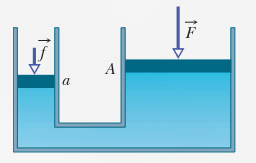
\includegraphics[width=0.45\linewidth]{images/28.png}
  \caption{Ilustrasi Tekanan Hidrolik nomor 28}
  \label{fig:hydraulic-press}
\end{figure}
 
\diketahui
\begin{align*}
d_k &= \SI{3,80}{\centi\metre}, &
d_b &= \SI{53,0}{\centi\metre}, &
F &= \SI{20,0}{\kilo\newton} = \SI{2,00e4}{\newton}
\end{align*}
 
\ditanya\ (a) $F$ dalam $f$, $a$, $A$; (b) $f$ pada piston kecil.
 
\konsep\ Prinsip Pascal: pertambahan tekanan pada fluida tertutup diteruskan sama besar ke
seluruh bagian fluida, sehingga $f/a = F/A$.
 
\penyelesaian
 
\textbf{(a)}
\begin{equation}
\frac{f}{a} = \frac{F}{A} \quad\Longrightarrow\quad F = f\,\frac{A}{a}
\end{equation}
Karena $A > a$, gaya kecil $f$ dapat menyeimbangkan gaya besar $F$.
 
\textbf{(b)} Luas piston sebanding dengan kuadrat diameter ($A = \pi d^2/4$), sehingga
\begin{align}
f &= F\,\frac{a}{A} = F \left(\frac{d_k}{d_b}\right)^2
 = (\SI{2,00e4}{\newton})\left(\frac{\SI{3,80}{\centi\metre}}{\SI{53,0}{\centi\metre}}\right)^2 \\
 &= (\SI{2,00e4}{\newton})(\num{5,14e-3}) = \SI{1,03e2}{\newton}
\end{align}
 
\begin{jawaban}
(a) $F = f\,A/a$.\\
(b) $f \approx \SI{1,03e2}{\newton}$.
\end{jawaban}
 
% =====================================================
\section*{Soal 29}
Pada Gambar 9, sebuah pegas dengan konstanta $\SI{3,00e4}{\newton\per\metre}$ berada
di antara balok kaku dan piston keluaran sebuah pengungkit hidrolik. Sebuah wadah kosong
bermassa dapat diabaikan diletakkan di atas piston masukan. Luas piston masukan $A_i$ dan
luas piston keluaran $18{,}0\,A_i$. Mula-mula pegas berada pada panjang alaminya. Berapa
kilogram pasir yang harus dituangkan (perlahan) ke wadah agar pegas tertekan sejauh
$\SI{5,00}{\centi\metre}$?

\begin{figure}[H]
  \centering
  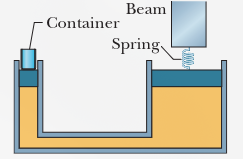
\includegraphics[width=0.45\linewidth]{images/29.png}
  \caption{Ilustrasi Pengungkit Hidrolik nomor 29}
  \label{fig:hydraulic}
\end{figure}
 
\diketahui
\begin{align*}
k &= \SI{3,00e4}{\newton\per\metre}, &
x &= \SI{5,00}{\centi\metre} = \SI{5,00e-2}{\metre}, &
A_o &= 18{,}0\,A_i
\end{align*}
 
\ditanya\ Massa pasir $m$.
 
\konsep\ Pegas yang tertekan sejauh $x$ memberi gaya $F_o = kx$ pada piston keluaran.
Pada keadaan setimbang, prinsip Pascal memberi $F_i/A_i = F_o/A_o$, dan gaya masukan berasal
dari berat pasir: $F_i = mg$.
 
\penyelesaian
\begin{align}
F_o &= kx = (\SI{3,00e4}{\newton\per\metre})(\SI{5,00e-2}{\metre}) = \SI{1,50e3}{\newton} \\
F_i &= F_o\,\frac{A_i}{A_o} = \frac{\SI{1,50e3}{\newton}}{\num{18,0}} = \SI{83,3}{\newton} \\
m &= \frac{F_i}{g} = \frac{\SI{83,3}{\newton}}{\SI{9,8}{\meter\per\second\squared}} = \SI{8,50}{\kilo\gram}
\end{align}
 
\begin{jawaban}
$m \approx \SI{8,50}{\kilo\gram}$.
\end{jawaban}
 
% =====================================================
\section*{Soal 30}
Sebuah benda $\SI{5,00}{\kilo\gram}$ dilepaskan dari keadaan diam saat tercelup penuh di
dalam suatu cairan. Cairan yang dipindahkan oleh benda memiliki massa $\SI{3,00}{\kilo\gram}$.
Seberapa jauh dan ke arah mana benda bergerak dalam $\SI{0,200}{\second}$, dengan anggapan
benda bergerak bebas dan gaya hambat cairan dapat diabaikan?
 
\diketahui
\begin{align*}
m &= \SI{5,00}{\kilo\gram}, &
m_{\text{cair}} &= \SI{3,00}{\kilo\gram}, &
t &= \SI{0,200}{\second}, &
v_0 &= 0
\end{align*}
 
\ditanya\ Perpindahan $y$ dan arahnya.
 
\konsep\ Hukum Archimedes: gaya apung $F_b = m_{\text{cair}}\, g$ (berat cairan yang
dipindahkan). Gaya neto $= mg - F_b$ menentukan percepatan; gerak lurus berubah beraturan.
 
\penyelesaian
\begin{align}
W &= mg = (\num{5,00})(\num{9,8}) = \SI{49,0}{\newton} \quad \text{(ke bawah)} \\
F_b &= m_{\text{cair}} g = (\num{3,00})(\num{9,8}) = \SI{29,4}{\newton} \quad \text{(ke atas)} \\
F_{\text{neto}} &= W - F_b = \SI{19,6}{\newton} \quad \text{(ke bawah)} \\
a &= \frac{F_{\text{neto}}}{m} = \frac{\SI{19,6}{\newton}}{\SI{5,00}{\kilo\gram}} = \SI{3,92}{\meter\per\second\squared} \\
y &= \tfrac{1}{2} a t^2 = \tfrac{1}{2}(\num{3,92})(\num{0,200})^2 = \SI{7,84e-2}{\metre}
\end{align}
 
\begin{jawaban}
Benda bergerak \emph{ke bawah} sejauh $\SI{7,84}{\centi\metre}$ ($\approx \SI{7,8e-2}{\metre}$).
\end{jawaban}

\section*{Soal 31}
Sebuah balok kayu mengapung di air tawar dengan dua pertiga volumenya $V$ tercelup, dan
mengapung di dalam minyak dengan $0{,}90V$ tercelup. Tentukan massa jenis (a) kayu dan
(b) minyak.
 
\diketahui
\begin{align*}
V_{\text{tercelup, air}} &= \tfrac{2}{3}V, &
V_{\text{tercelup, minyak}} &= 0{,}90\,V, &
\rho_{\text{air}} &= \SI{1,00e3}{\kilo\gram\per\metre\cubed}
\end{align*}
 
\ditanya\ (a) $\rho_{\text{kayu}}$; (b) $\rho_{\text{minyak}}$.
 
\konsep\ Benda mengapung (setimbang) bila gaya apung sama dengan beratnya:
$\rho_{\text{fluida}}\, V_{\text{tercelup}}\, g = \rho_{\text{benda}}\, V g$.
 
\penyelesaian
 
\textbf{(a)} Di air:
\begin{equation}
\rho_{\text{kayu}} V g = \rho_{\text{air}} \left(\tfrac{2}{3}V\right) g
\ \Longrightarrow\
\rho_{\text{kayu}} = \tfrac{2}{3}\,(\SI{1,00e3}{\kilo\gram\per\metre\cubed}) = \SI{6,7e2}{\kilo\gram\per\metre\cubed}
\end{equation}
 
\textbf{(b)} Di minyak:
\begin{equation}
\rho_{\text{kayu}} V g = \rho_{\text{minyak}} (0{,}90V) g
\ \Longrightarrow\
\rho_{\text{minyak}} = \frac{\SI{667}{\kilo\gram\per\metre\cubed}}{\num{0,90}} = \SI{7,4e2}{\kilo\gram\per\metre\cubed}
\end{equation}
 
\begin{jawaban}
(a) $\rho_{\text{kayu}} \approx \SI{6,7e2}{\kilo\gram\per\metre\cubed}$.\\
(b) $\rho_{\text{minyak}} \approx \SI{7,4e2}{\kilo\gram\per\metre\cubed}$.
\end{jawaban}
 
% =====================================================
\section*{Soal 32}
Pada Gambar 10, sebuah kubus bersisi $L = \SI{0,600}{\metre}$ dan bermassa
$\SI{450}{\kilo\gram}$ digantung dengan tali di dalam tangki terbuka berisi cairan bermassa
jenis $\SI{1030}{\kilo\gram\per\metre\cubed}$. Tentukan (a) besar gaya total ke bawah pada
sisi atas kubus dari cairan dan atmosfer (tekanan atmosfer $\SI{1,00}{\atm}$),
(b) besar gaya total ke atas pada sisi bawah kubus, dan (c) tegangan tali.
(d) Hitung gaya apung dengan prinsip Archimedes. Hubungan apa yang berlaku di antara
semua besaran tersebut?

\begin{figure}[H]
  \centering
  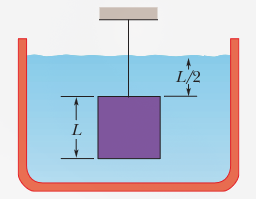
\includegraphics[width=0.45\linewidth]{images/32.png}
  \caption{Ilustrasi Kubus dalam Cairan nomor 32}
  \label{fig:cube}
\end{figure}
 
\diketahui\ (dari Gambar 10, sisi atas kubus berada $L/2$ di bawah permukaan cairan)
\begin{align*}
L &= \SI{0,600}{\metre}, &
m &= \SI{450}{\kilo\gram}, &
\rho &= \SI{1030}{\kilo\gram\per\metre\cubed}\\
p_0 &= \SI{1,00}{\atm} = \SI{1,013e5}{\pascal}, &
A &= L^2 = \SI{0,360}{\metre\squared}
\end{align*}
 
\ditanya\ (a) $F_{\text{atas}}$; (b) $F_{\text{bawah}}$; (c) $T$; (d) $F_b$.
 
\konsep\ Tekanan pada kedalaman $y$: $p = p_0 + \rho g y$. Sisi atas berada pada kedalaman
$L/2 = \SI{0,300}{\metre}$ dan sisi bawah pada $3L/2 = \SI{0,900}{\metre}$.
 
\penyelesaian
 
\textbf{(a)} Gaya pada sisi atas:
\begin{align}
p_{\text{atas}} &= p_0 + \rho g \tfrac{L}{2}
 = \SI{1,013e5}{\pascal} + (\num{1030})(\num{9,8})(\num{0,300}) = \SI{1,043e5}{\pascal} \\
F_{\text{atas}} &= p_{\text{atas}} A = (\SI{1,043e5}{\pascal})(\SI{0,360}{\metre\squared}) = \SI{3,76e4}{\newton}
\end{align}
 
\textbf{(b)} Gaya pada sisi bawah:
\begin{align}
p_{\text{bawah}} &= p_0 + \rho g \tfrac{3L}{2}
 = \SI{1,013e5}{\pascal} + (\num{1030})(\num{9,8})(\num{0,900}) = \SI{1,104e5}{\pascal} \\
F_{\text{bawah}} &= p_{\text{bawah}} A = (\SI{1,104e5}{\pascal})(\SI{0,360}{\metre\squared}) = \SI{3,97e4}{\newton}
\end{align}
 
\textbf{(c)} Kubus setimbang: $T + F_{\text{bawah}} = mg + F_{\text{atas}}$, sehingga
\begin{align}
T &= mg - \left(F_{\text{bawah}} - F_{\text{atas}}\right) \\
  &= (\num{450})(\num{9,8}) - \left(\SI{3,974e4}{\newton} - \SI{3,756e4}{\newton}\right)
   = \SI{4410}{\newton} - \SI{2180}{\newton} = \SI{2,23e3}{\newton}
\end{align}
 
\textbf{(d)} Gaya apung menurut Archimedes (berat cairan yang dipindahkan):
\begin{equation}
F_b = \rho g V = \rho g L^3 = (\num{1030})(\num{9,8})(\num{0,600})^3 = \SI{2,18e3}{\newton}
\end{equation}
 
\textbf{Hubungan:} Gaya apung sama dengan selisih gaya tekan pada sisi bawah dan sisi atas,
$F_b = F_{\text{bawah}} - F_{\text{atas}}$, dan tegangan tali memenuhi $T = mg - F_b$.
 
\begin{jawaban}
(a) $F_{\text{atas}} \approx \SI{3,76e4}{\newton}$.\\
(b) $F_{\text{bawah}} \approx \SI{3,97e4}{\newton}$.\\
(c) $T \approx \SI{2,23e3}{\newton}$.\\
(d) $F_b \approx \SI{2,18e3}{\newton} = F_{\text{bawah}} - F_{\text{atas}}$.
\end{jawaban}
 
% =====================================================
\section*{Soal 33}
Sebuah jangkar besi bermassa jenis $\SI{7870}{\kilo\gram\per\metre\cubed}$ tampak lebih ringan
$\SI{200}{\newton}$ di dalam air dibandingkan di udara. (a) Berapa volume jangkar?
(b) Berapa berat jangkar di udara?
 
\diketahui
\begin{align*}
\rho_{\text{besi}} &= \SI{7870}{\kilo\gram\per\metre\cubed}, &
\Delta W &= \SI{200}{\newton}, &
\rho_{\text{air}} &= \SI{1,00e3}{\kilo\gram\per\metre\cubed}
\end{align*}
 
\ditanya\ (a) $V$; (b) $W_{\text{udara}}$.
 
\konsep\ Berat semu di air lebih kecil daripada berat di udara sebesar gaya apung:
$\Delta W = F_b = \rho_{\text{air}}\, g\, V$.
 
\penyelesaian
 
\textbf{(a)}
\begin{equation}
V = \frac{F_b}{\rho_{\text{air}}\, g} = \frac{\SI{200}{\newton}}{(\SI{1,00e3}{\kilo\gram\per\metre\cubed})(\SI{9,8}{\meter\per\second\squared})}
 = \SI{2,04e-2}{\metre\cubed}
\end{equation}
 
\textbf{(b)}
\begin{equation}
W_{\text{udara}} = \rho_{\text{besi}}\, g\, V = (\num{7870})(\num{9,8})(\num{2,04e-2}) = \SI{1,57e3}{\newton}
\end{equation}
 
\begin{jawaban}
(a) $V \approx \SI{2,04e-2}{\metre\cubed}$.\\
(b) $W_{\text{udara}} \approx \SI{1,57e3}{\newton}$.
\end{jawaban}
 
% =====================================================
\section*{Soal 34}
Sebuah perahu yang mengapung di air tawar memindahkan air seberat $\SI{35,6}{\kilo\newton}$.
(a) Berapa berat air yang dipindahkan bila perahu mengapung di air laut bermassa jenis
$\SI{1,10e3}{\kilo\gram\per\metre\cubed}$? (b) Berapa selisih volume air tawar yang
dipindahkan dan volume air laut yang dipindahkan?
 
\diketahui
\begin{align*}
W_{\text{tawar}} &= \SI{35,6}{\kilo\newton} = \SI{3,56e4}{\newton}, &
\rho_{\text{tawar}} &= \SI{1,00e3}{\kilo\gram\per\metre\cubed}, &
\rho_{\text{laut}} &= \SI{1,10e3}{\kilo\gram\per\metre\cubed}
\end{align*}
 
\ditanya\ (a) $W_{\text{laut}}$; (b) $V_{\text{tawar}} - V_{\text{laut}}$.
 
\konsep\ Perahu mengapung sehingga gaya apung sama dengan berat perahu; menurut Archimedes,
gaya apung sama dengan berat fluida yang dipindahkan. Volume fluida yang dipindahkan
$V = W_{\text{perahu}}/(\rho g)$.
 
\penyelesaian
 
\textbf{(a)} Berat perahu tidak berubah, sehingga berat air yang dipindahkan sama:
$W_{\text{laut}} = W_{\text{tawar}} = \SI{35,6}{\kilo\newton}$.
 
\textbf{(b)}
\begin{align}
V_{\text{tawar}} &= \frac{\SI{3,56e4}{\newton}}{(\num{1,00e3})(\num{9,8})} = \SI{3,63}{\metre\cubed} \\
V_{\text{laut}} &= \frac{\SI{3,56e4}{\newton}}{(\num{1,10e3})(\num{9,8})} = \SI{3,30}{\metre\cubed} \\
\Delta V &= V_{\text{tawar}} - V_{\text{laut}} = \SI{0,33}{\metre\cubed}
\end{align}
 
\begin{jawaban}
(a) $W_{\text{laut}} = \SI{35,6}{\kilo\newton}$.\\
(b) $\Delta V \approx \SI{0,33}{\metre\cubed}$ (di air tawar perahu memindahkan volume lebih besar).
\end{jawaban}
 
% =====================================================
\section*{Soal 35}
Tiga anak, masing-masing berat $\SI{356}{\newton}$, membuat rakit dengan mengikat
gelondongan kayu berdiameter $\SI{0,30}{\metre}$ dan panjang $\SI{1,80}{\metre}$.
Berapa gelondongan yang diperlukan agar mereka tetap mengapung di air tawar? Massa jenis
kayu $\SI{800}{\kilo\gram\per\metre\cubed}$.
 
\diketahui
\begin{align*}
W_{\text{anak}} &= 3(\SI{356}{\newton}) = \SI{1068}{\newton}\\
d &= \SI{0,30}{\metre}\ (r = \SI{0,15}{\metre}), &
l &= \SI{1,80}{\metre}\\
\rho_{\text{kayu}} &= \SI{800}{\kilo\gram\per\metre\cubed}, &
\rho_{\text{air}} &= \SI{1,00e3}{\kilo\gram\per\metre\cubed}
\end{align*}
 
\ditanya\ Jumlah gelondongan minimum $N$.
 
\konsep\ Kondisi batas: rakit tepat tercelup penuh. Gaya apung maksimum tiap gelondongan
$\rho_{\text{air}} g V$ harus menyangga berat gelondongan sendiri $\rho_{\text{kayu}} g V$
ditambah beban anak-anak:
\begin{equation*}
N\left(\rho_{\text{air}} - \rho_{\text{kayu}}\right) g V \ge W_{\text{anak}}
\end{equation*}
 
\penyelesaian
\begin{align}
V &= \pi r^2 l = \pi (\SI{0,15}{\metre})^2 (\SI{1,80}{\metre}) = \SI{0,127}{\metre\cubed} \\
\left(\rho_{\text{air}} - \rho_{\text{kayu}}\right) g V
 &= (\num{200})(\num{9,8})(\num{0,127}) = \SI{249}{\newton} \quad \text{(per gelondongan)} \\
N &\ge \frac{\SI{1068}{\newton}}{\SI{249}{\newton}} = \num{4,28}
\end{align}
Jumlah gelondongan harus bilangan bulat, sehingga dibulatkan ke atas.
 
\begin{jawaban}
$N = 5$ gelondongan.
\end{jawaban}

\section*{Soal 36}
Pada Gambar 11a, sebuah balok persegi panjang didorong perlahan dengan sisi bawah
menghadap ke bawah ke dalam suatu cairan. Balok memiliki tinggi $d$; luas sisi bawah dan
sisi atasnya $A = \SI{5,67}{\centi\metre\squared}$. Gambar 9b memberikan berat semu
$W_{\text{app}}$ balok sebagai fungsi kedalaman $h$ sisi bawahnya. Skala sumbu vertikal
ditentukan oleh $W_s = \SI{0,20}{\newton}$. Berapa massa jenis cairan?

\begin{figure}[H]
  \centering
  \begin{subfigure}{0.45\linewidth}
    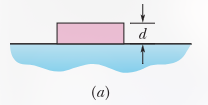
\includegraphics[width=\linewidth]{images/36a.png}
    \caption{Balok didorong ke cairan}
  \end{subfigure}
  \hfill
  \begin{subfigure}{0.45\linewidth}
    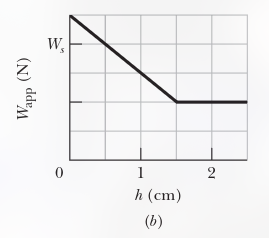
\includegraphics[width=\linewidth]{images/36b.png}
    \caption{Grafik $W_{\text{app}}$ terhadap $h$}
  \end{subfigure}
  \caption{Gambar untuk Soal 36.}
\end{figure}
 
\diketahui\ (dibaca dari grafik Gambar 11b; tiap kotak vertikal bernilai $W_s/4 = \SI{0,05}{\newton}$)
\begin{align*}
W_{\text{udara}} &= W_{\text{app}}(h = 0) = \SI{0,25}{\newton}\\
W_{\text{app,min}} &= \SI{0,10}{\newton} \quad \text{(konstan untuk } h \ge \SI{1,5}{\centi\metre}\text{)}\\
d &= \SI{1,5}{\centi\metre} = \SI{1,5e-2}{\metre} \quad \text{(balok tepat tercelup penuh)}\\
A &= \SI{5,67}{\centi\metre\squared} = \SI{5,67e-4}{\metre\squared}
\end{align*}
 
\ditanya\ Massa jenis cairan $\rho_c$.
 
\konsep\ Berat semu sama dengan berat di udara dikurangi gaya apung:
$W_{\text{app}} = W - F_b$. Setelah balok tercelup penuh ($h \ge d$), gaya apung konstan
sehingga $W_{\text{app}}$ konstan. Gaya apung maksimum $F_b = \rho_c\, g\, V$ dengan
$V = A d$.
 
\penyelesaian
\begin{align}
F_b &= W - W_{\text{app,min}} = \SI{0,25}{\newton} - \SI{0,10}{\newton} = \SI{0,15}{\newton} \\
V &= A d = (\SI{5,67e-4}{\metre\squared})(\SI{1,5e-2}{\metre}) = \SI{8,51e-6}{\metre\cubed} \\
\rho_c &= \frac{F_b}{g V} = \frac{\SI{0,15}{\newton}}{(\SI{9,8}{\meter\per\second\squared})(\SI{8,51e-6}{\metre\cubed})}
 = \SI{1,8e3}{\kilo\gram\per\metre\cubed}
\end{align}
 
\begin{jawaban}
$\rho_c \approx \SI{1,8e3}{\kilo\gram\per\metre\cubed}$.
\end{jawaban}
 
% =====================================================
\section*{Soal 37}
Sebuah cangkang bola besi berongga mengapung hampir tenggelam seluruhnya di dalam air.
Diameter luarnya $\SI{60,0}{\centi\metre}$ dan massa jenis besi $\SI{7,87}{\gram\per\cubic\centi\metre}$.
Tentukan diameter dalamnya.
 
\diketahui
\begin{align*}
d_o &= \SI{60,0}{\centi\metre} \ (r_o = \SI{30,0}{\centi\metre}), &
\rho_{\text{besi}} &= \SI{7,87}{\gram\per\cubic\centi\metre}, &
\rho_{\text{air}} &= \SI{1,00}{\gram\per\cubic\centi\metre}
\end{align*}
 
\ditanya\ Diameter dalam $d_i$.
 
\konsep\ Cangkang mengapung dengan hampir seluruh volume luarnya tercelup, sehingga gaya
apung $= \rho_{\text{air}}\, g\, V_o$ dan sama dengan berat cangkang
$\rho_{\text{besi}}\, g\,(V_o - V_i)$, dengan $V_o = \tfrac{4}{3}\pi r_o^3$ dan
$V_i = \tfrac{4}{3}\pi r_i^3$.
 
\penyelesaian
\begin{align}
\rho_{\text{besi}}\,(r_o^3 - r_i^3) &= \rho_{\text{air}}\, r_o^3 \\
r_i^3 &= r_o^3\left(1 - \frac{\rho_{\text{air}}}{\rho_{\text{besi}}}\right)
 = (\SI{30,0}{\centi\metre})^3\left(1 - \frac{\num{1,00}}{\num{7,87}}\right) \\
r_i &= (\SI{30,0}{\centi\metre})(\num{0,8729})^{1/3} = (\SI{30,0}{\centi\metre})(\num{0,9557}) = \SI{28,7}{\centi\metre} \\
d_i &= 2 r_i = \SI{57,3}{\centi\metre}
\end{align}
 
\begin{jawaban}
$d_i \approx \SI{57,3}{\centi\metre}$.
\end{jawaban}
 
% =====================================================
\section*{Soal 38}
Sebuah bola padat kecil dilepaskan dari keadaan diam saat tercelup penuh di dalam suatu
cairan, lalu energi kinetiknya diukur ketika telah bergerak $\SI{4,0}{\centi\metre}$ di dalam
cairan. Gambar 12 memberikan hasil untuk banyak cairan: energi kinetik $K$ diplot
terhadap massa jenis cairan $\rho_{\text{cair}}$, dengan $K_s = \SI{1,60}{\joule}$ sebagai
skala sumbu vertikal. Tentukan (a) massa jenis dan (b) volume bola.

\begin{figure}[H]
  \centering
  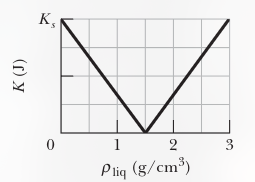
\includegraphics[width=0.45\linewidth]{images/38.png}
  \caption{Ilustrasi Bola Tercelup dalam Cairan 38}
  \label{fig:ball}
\end{figure}
 
\diketahui\ (dari grafik Gambar 12)
\begin{align*}
K = K_s &= \SI{1,60}{\joule} \quad \text{pada } \rho_{\text{cair}} = 0\\
K = 0 &\quad \text{pada } \rho_{\text{cair}} = \SI{1,5}{\gram\per\cubic\centi\metre}\\
s &= \SI{4,0}{\centi\metre} = \SI{4,0e-2}{\metre}
\end{align*}
 
\ditanya\ (a) $\rho_{\text{bola}}$; (b) $V$.
 
\konsep\ Karena dilepas dari keadaan diam dan hambatan diabaikan, energi kinetik sama dengan
usaha gaya neto sepanjang $s$:
\begin{equation*}
K = \left|m g - \rho_{\text{cair}}\, g V\right| s
\end{equation*}
$K = 0$ berarti gaya neto nol (bola melayang), yaitu saat $\rho_{\text{cair}} = \rho_{\text{bola}}$.
Untuk $\rho_{\text{cair}} = 0$ tidak ada gaya apung, sehingga $K = K_s = m g s$.
 
\penyelesaian
 
\textbf{(a)} Dari grafik, $K = 0$ pada $\rho_{\text{cair}} = \SI{1,5}{\gram\per\cubic\centi\metre}$, sehingga
\begin{equation}
\rho_{\text{bola}} = \SI{1,5}{\gram\per\cubic\centi\metre} = \SI{1,5e3}{\kilo\gram\per\metre\cubed}
\end{equation}
 
\textbf{(b)} Dari $K_s = m g s$:
\begin{align}
m &= \frac{K_s}{g s} = \frac{\SI{1,60}{\joule}}{(\SI{9,8}{\meter\per\second\squared})(\SI{4,0e-2}{\metre})} = \SI{4,08}{\kilo\gram} \\
V &= \frac{m}{\rho_{\text{bola}}} = \frac{\SI{4,08}{\kilo\gram}}{\SI{1,5e3}{\kilo\gram\per\metre\cubed}}
 = \SI{2,7e-3}{\metre\cubed}
\end{align}
 
\begin{jawaban}
(a) $\rho_{\text{bola}} \approx \SI{1,5e3}{\kilo\gram\per\metre\cubed}$.\\
(b) $V \approx \SI{2,7e-3}{\metre\cubed}$ (dengan $m \approx \SI{4,08}{\kilo\gram}$).
\end{jawaban}
 
% =====================================================
\section*{Soal 39}
Sebuah bola berongga dengan jari-jari dalam $\SI{8,0}{\centi\metre}$ dan jari-jari luar
$\SI{9,0}{\centi\metre}$ mengapung dengan setengah volumenya tercelup di dalam cairan
bermassa jenis $\SI{800}{\kilo\gram\per\metre\cubed}$. (a) Berapa massa bola?
(b) Hitung massa jenis bahan pembuat bola.
 
\diketahui
\begin{align*}
r_i &= \SI{8,0e-2}{\metre}, &
r_o &= \SI{9,0e-2}{\metre}, &
\rho_c &= \SI{800}{\kilo\gram\per\metre\cubed}
\end{align*}
 
\ditanya\ (a) $m$; (b) $\rho_{\text{bahan}}$.
 
\konsep\ Bola mengapung: gaya apung sama dengan berat. Volume tercelup
$\tfrac{1}{2}V_o$ dengan $V_o = \tfrac{4}{3}\pi r_o^3$ (volume luar). Volume bahan
$V_b = \tfrac{4}{3}\pi\left(r_o^3 - r_i^3\right)$.
 
\penyelesaian
 
\textbf{(a)}
\begin{align}
V_o &= \tfrac{4}{3}\pi (\SI{9,0e-2}{\metre})^3 = \SI{3,05e-3}{\metre\cubed} \\
m g &= \rho_c g \left(\tfrac{1}{2}V_o\right)
 \ \Longrightarrow\
m = (\SI{800}{\kilo\gram\per\metre\cubed})\left(\tfrac{1}{2}\right)(\SI{3,05e-3}{\metre\cubed}) = \SI{1,22}{\kilo\gram}
\end{align}
 
\textbf{(b)}
\begin{align}
V_b &= \tfrac{4}{3}\pi\left[(\SI{9,0e-2}{\metre})^3 - (\SI{8,0e-2}{\metre})^3\right] = \SI{9,09e-4}{\metre\cubed} \\
\rho_{\text{bahan}} &= \frac{m}{V_b} = \frac{\SI{1,22}{\kilo\gram}}{\SI{9,09e-4}{\metre\cubed}}
 = \SI{1,3e3}{\kilo\gram\per\metre\cubed}
\end{align}
 
\begin{jawaban}
(a) $m \approx \SI{1,2}{\kilo\gram}$.\\
(b) $\rho_{\text{bahan}} \approx \SI{1,3e3}{\kilo\gram\per\metre\cubed}$.
\end{jawaban}
 
% =====================================================
\section*{Soal 40}
\textit{Aligator yang mengintai.} Seekor aligator menunggu mangsa dengan mengapung sehingga
hanya bagian atas kepalanya yang tampak. Salah satu cara menyesuaikan tingkat
tenggelamnya adalah dengan menelan batu (\textit{gastrolit}) yang tinggal di lambungnya.
Gambar 13 memperlihatkan model sangat sederhana (``\textit{rhombohedron gater}'')
bermassa $\SI{130}{\kilo\gram}$ dengan kepala sebagian muncul di permukaan. Luas permukaan
atas kepala $\SI{0,20}{\metre\squared}$. Jika aligator menelan batu dengan massa total
$\SI{1,0}{\percent}$ dari massa tubuhnya (jumlah yang lazim), seberapa jauh ia tenggelam?

\begin{figure}[H]
  \centering
  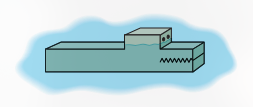
\includegraphics[width=0.45\linewidth]{images/40.png}
  \caption{Ilustrasi Aligator Mengintai nomor 40}
  \label{fig:alligator-spying}
\end{figure}
 
\diketahui
\begin{align*}
M &= \SI{130}{\kilo\gram}, &
m_{\text{batu}} &= 0{,}010\,M = \SI{1,3}{\kilo\gram}, &
A &= \SI{0,20}{\metre\squared}, &
\rho_{\text{air}} &= \SI{1,00e3}{\kilo\gram\per\metre\cubed}
\end{align*}
 
\ditanya\ Pertambahan kedalaman tenggelam $\Delta y$.
 
\konsep\ Aligator tetap mengapung (setimbang), sehingga pertambahan berat harus diimbangi
pertambahan gaya apung. Bagian kepala yang berada di permukaan dianggap memiliki
penampang tetap $A$ sehingga tambahan volume tercelup $\Delta V = A\,\Delta y$:
\begin{equation*}
m_{\text{batu}}\, g = \rho_{\text{air}}\, g\, A\, \Delta y
\end{equation*}
 
\penyelesaian
\begin{equation}
\Delta y = \frac{m_{\text{batu}}}{\rho_{\text{air}} A}
 = \frac{\SI{1,3}{\kilo\gram}}{(\SI{1,00e3}{\kilo\gram\per\metre\cubed})(\SI{0,20}{\metre\squared})}
 = \SI{6,5e-3}{\metre}
\end{equation}
 
\begin{jawaban}
$\Delta y \approx \SI{6,5}{\milli\metre}$ (aligator tenggelam sedalam $\SI{6,5}{\milli\metre}$ lebih jauh).
\end{jawaban}

\section*{Soal 41}
Berapa bagian volume gunung es (massa jenis $\SI{917}{\kilo\gram\per\metre\cubed}$) yang
tampak di atas permukaan bila gunung es mengapung (a) di samudra (air laut bermassa jenis
$\SI{1024}{\kilo\gram\per\metre\cubed}$) dan (b) di sungai (air tawar bermassa jenis
$\SI{1000}{\kilo\gram\per\metre\cubed}$)?
 
\diketahui
\begin{align*}
\rho_{\text{es}} &= \SI{917}{\kilo\gram\per\metre\cubed}, &
\rho_{\text{laut}} &= \SI{1024}{\kilo\gram\per\metre\cubed}, &
\rho_{\text{tawar}} &= \SI{1000}{\kilo\gram\per\metre\cubed}
\end{align*}
 
\ditanya\ Fraksi volume yang tampak $f_{\text{tampak}}$ untuk (a) dan (b).
 
\konsep\ Benda mengapung: $\rho_{\text{es}}\, V g = \rho_{\text{fluida}}\, V_{\text{tercelup}}\, g$, sehingga
fraksi tercelup $V_{\text{tercelup}}/V = \rho_{\text{es}}/\rho_{\text{fluida}}$ dan
\begin{equation*}
f_{\text{tampak}} = 1 - \frac{\rho_{\text{es}}}{\rho_{\text{fluida}}}
\end{equation*}
 
\penyelesaian
 
\textbf{(a)} Di samudra:
\begin{equation}
f_{\text{tampak}} = 1 - \frac{\num{917}}{\num{1024}} = \num{0,104}
\end{equation}
 
\textbf{(b)} Di sungai:
\begin{equation}
f_{\text{tampak}} = 1 - \frac{\num{917}}{\num{1000}} = \num{0,083}
\end{equation}
 
\begin{jawaban}
(a) $f_{\text{tampak}} \approx \num{0,104}$ (sekitar \SI{10,4}{\percent}).\\
(b) $f_{\text{tampak}} \approx \num{0,083}$ (sekitar \SI{8,3}{\percent}).
\end{jawaban}
 
% =====================================================
\section*{Soal 42}
Sebuah alat apung berbentuk silinder tegak dengan tinggi $\SI{0,500}{\metre}$ dan luas
penampang atas serta bawah $\SI{4,00}{\metre\squared}$; massa jenisnya $0{,}400$ kali massa
jenis air tawar. Mula-mula alat ditahan tercelup penuh di air tawar dengan sisi atasnya tepat
di permukaan air. Kemudian alat dibiarkan naik perlahan hingga mulai mengapung. Berapa usaha
yang dilakukan gaya apung pada alat selama gerakan naik tersebut?
 
\diketahui
\begin{align*}
h &= \SI{0,500}{\metre}, &
A &= \SI{4,00}{\metre\squared}, &
\rho &= 0{,}400\,\rho_{\text{air}} = \SI{400}{\kilo\gram\per\metre\cubed}, &
\rho_{\text{air}} &= \SI{1,00e3}{\kilo\gram\per\metre\cubed}
\end{align*}
 
\ditanya\ Usaha gaya apung $W_b$ selama alat naik dari tercelup penuh sampai mengapung.
 
\konsep\ Saat mengapung, fraksi tercelup $= \rho/\rho_{\text{air}} = 0{,}400$, sehingga tinggi
bagian tercelup $h_{\text{tc}} = 0{,}400\,(\SI{0,500}{\metre}) = \SI{0,200}{\metre}$. Alat harus naik
sejauh
\begin{equation*}
\Delta y = h - h_{\text{tc}} = \SI{0,500}{\metre} - \SI{0,200}{\metre} = \SI{0,300}{\metre}
\end{equation*}
Selama naik sejauh $y$, tinggi bagian tercelup adalah $h - y$, sehingga gaya apung
berkurang linear: $F_b(y) = \rho_{\text{air}}\, g\, A\,(h - y)$.
 
\penyelesaian
\begin{align}
W_b &= \int_{0}^{\Delta y} \rho_{\text{air}}\, g\, A\,(h - y)\, dy
 = \rho_{\text{air}}\, g\, A \left[h\,\Delta y - \tfrac{1}{2}\Delta y^2\right] \\
 &= (\num{1,00e3})(\num{9,8})(\num{4,00})\left[(\num{0,500})(\num{0,300}) - \tfrac{1}{2}(\num{0,300})^2\right] \\
 &= (\SI{3,92e4}{\newton\per\metre})(\SI{0,105}{\metre\squared}) = \SI{4,12e3}{\joule}
\end{align}
(Cara lain: gaya apung awal $\SI{1,96e4}{\newton}$, akhir $\SI{7,84e3}{\newton}$, rata-rata
$\SI{1,37e4}{\newton}$ dikali $\SI{0,300}{\metre}$ menghasilkan nilai yang sama.)
 
\begin{jawaban}
$W_b \approx \SI{4,1e3}{\joule}$.
\end{jawaban}
 
% =====================================================
\section*{Soal 43}
Ketika peneliti menemukan fosil dinosaurus yang cukup lengkap, mereka dapat menentukan
massa dan berat dinosaurus hidup dengan model berskala yang dibuat dari plastik berdasarkan
dimensi tulang fosil. Skala model $1/20$: panjang model $1/20$ panjang sebenarnya, luas
$(1/20)^2$ kali luas sebenarnya, dan volume $(1/20)^3$ kali volume sebenarnya. Pertama,
model digantung pada satu lengan neraca dan anak timbangan ditambahkan pada lengan lain
sampai setimbang. Kemudian model tercelup penuh dalam air dan sejumlah anak timbangan
dikurangi dari lengan kedua agar setimbang kembali (Gambar 14). Untuk model sebuah fosil
\textit{T.\ rex}, $\SI{637,76}{\gram}$ harus dikurangi. Berapa volume (a) model dan (b)
\textit{T.\ rex} sebenarnya? (c) Jika massa jenis \textit{T.\ rex} kira-kira sama dengan
massa jenis air, berapa massanya?

\begin{figure}[H]
  \centering
  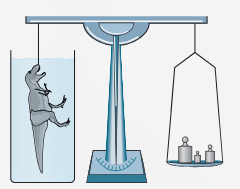
\includegraphics[width=0.45\linewidth]{images/43.png}
  \caption{Ilustrasi Fosil Tercelup Dibanding Beban nomor 43}
  \label{fig:fossil}
\end{figure}
 
\diketahui
\begin{align*}
m_{\text{kurang}} &= \SI{637,76}{\gram} = \SI{0,63776}{\kilo\gram}, &
\text{skala} &= \tfrac{1}{20}, &
\rho_{\text{air}} &= \SI{1,00e3}{\kilo\gram\per\metre\cubed}
\end{align*}
 
\ditanya\ (a) $V_{\text{model}}$; (b) $V_{\text{T.rex}}$; (c) $m_{\text{T.rex}}$.
 
\konsep\ Berat anak timbangan yang dikurangi sama dengan gaya apung pada model yang
tercelup penuh: $m_{\text{kurang}}\, g = \rho_{\text{air}}\, g\, V_{\text{model}}$. Volume sebenarnya
$= 20^3 \times$ volume model.
 
\penyelesaian
 
\textbf{(a)}
\begin{equation}
V_{\text{model}} = \frac{m_{\text{kurang}}}{\rho_{\text{air}}}
 = \frac{\SI{0,63776}{\kilo\gram}}{\SI{1,00e3}{\kilo\gram\per\metre\cubed}} = \SI{6,38e-4}{\metre\cubed}
\end{equation}
 
\textbf{(b)}
\begin{equation}
V_{\text{T.rex}} = 20^3\, V_{\text{model}} = (\num{8000})(\SI{6,3776e-4}{\metre\cubed}) = \SI{5,10}{\metre\cubed}
\end{equation}
 
\textbf{(c)}
\begin{equation}
m_{\text{T.rex}} = \rho_{\text{air}}\, V_{\text{T.rex}} = (\SI{1,00e3}{\kilo\gram\per\metre\cubed})(\SI{5,10}{\metre\cubed}) = \SI{5,10e3}{\kilo\gram}
\end{equation}
 
\begin{jawaban}
(a) $V_{\text{model}} \approx \SI{6,38e-4}{\metre\cubed}$.\\
(b) $V_{\text{T.rex}} \approx \SI{5,10}{\metre\cubed}$.\\
(c) $m_{\text{T.rex}} \approx \SI{5,10e3}{\kilo\gram}$.
\end{jawaban}
 
% =====================================================
\section*{Soal 44}
Sebuah balok kayu (massa $\SI{3,67}{\kilo\gram}$, massa jenis $\SI{600}{\kilo\gram\per\metre\cubed}$)
dipasangi timbal (massa jenis $\SI{1,14e4}{\kilo\gram\per\metre\cubed}$) sehingga mengapung
di air dengan $0{,}900$ volumenya tercelup. Tentukan massa timbal bila timbal dipasang pada
(a) sisi atas dan (b) sisi bawah balok.
 
\diketahui
\begin{align*}
m_k &= \SI{3,67}{\kilo\gram}, &
\rho_k &= \SI{600}{\kilo\gram\per\metre\cubed}, &
\rho_t &= \SI{1,14e4}{\kilo\gram\per\metre\cubed}, &
\rho_{\text{air}} &= \SI{1,00e3}{\kilo\gram\per\metre\cubed}
\end{align*}
 
\ditanya\ Massa timbal $m_t$ untuk (a) timbal di atas dan (b) timbal di bawah.
 
\konsep\ Volume kayu $V_k = m_k/\rho_k = \SI{6,12e-3}{\metre\cubed}$; volume kayu yang
tercelup $0{,}900\,V_k$. Pada keadaan mengapung, gaya apung total sama dengan berat total.
 
\penyelesaian
 
\textbf{(a) Timbal di atas} (timbal berada di atas air sehingga tidak ikut tercelup):
\begin{align}
\rho_{\text{air}}\,(0{,}900\,V_k)\,g &= (m_k + m_t)\,g \\
m_t &= \rho_{\text{air}}(0{,}900\,V_k) - m_k
 = (\num{1,00e3})(\num{0,900})(\SI{6,12e-3}{\metre\cubed}) - \SI{3,67}{\kilo\gram} \\
 &= \SI{5,505}{\kilo\gram} - \SI{3,67}{\kilo\gram} = \SI{1,84}{\kilo\gram}
\end{align}
 
\textbf{(b) Timbal di bawah} (timbal ikut tercelup, volumenya $V_t = m_t/\rho_t$ juga
mendapat gaya apung):
\begin{align}
\rho_{\text{air}}\left(0{,}900\,V_k + \frac{m_t}{\rho_t}\right) &= m_k + m_t \\
\SI{5,505}{\kilo\gram} + m_t\,\frac{\rho_{\text{air}}}{\rho_t} &= \SI{3,67}{\kilo\gram} + m_t \\
m_t\left(1 - \frac{\num{1,00e3}}{\num{1,14e4}}\right) &= \SI{5,505}{\kilo\gram} - \SI{3,67}{\kilo\gram} = \SI{1,835}{\kilo\gram} \\
m_t &= \frac{\SI{1,835}{\kilo\gram}}{\num{0,9123}} = \SI{2,01}{\kilo\gram}
\end{align}
 
\begin{jawaban}
(a) $m_t \approx \SI{1,84}{\kilo\gram}$ (timbal di atas).\\
(b) $m_t \approx \SI{2,01}{\kilo\gram}$ (timbal di bawah).
\end{jawaban}
 
% =====================================================
\section*{Soal 45}
Sebuah coran besi yang mengandung sejumlah rongga memiliki berat $\SI{6000}{\newton}$ di
udara dan $\SI{4000}{\newton}$ di dalam air. Berapa total volume rongga pada coran tersebut?
Massa jenis besi padat $\SI{7,87}{\gram\per\cubic\centi\metre}$.
 
\diketahui
\begin{align*}
W_{\text{udara}} &= \SI{6000}{\newton}, &
W_{\text{air}} &= \SI{4000}{\newton}, &
\rho_{\text{besi}} &= \SI{7,87e3}{\kilo\gram\per\metre\cubed}
\end{align*}
 
\ditanya\ Volume rongga total $V_r$.
 
\konsep\ Selisih berat di udara dan di air adalah gaya apung, yang bergantung pada volume
\emph{total} coran (besi + rongga): $F_b = \rho_{\text{air}}\, g\, V_{\text{total}}$.
Volume besi saja ditentukan dari beratnya (rongga dianggap kosong dan tak bermassa):
$V_{\text{besi}} = W_{\text{udara}}/(\rho_{\text{besi}}\, g)$. Maka $V_r = V_{\text{total}} - V_{\text{besi}}$.
 
\penyelesaian
\begin{align}
F_b &= \SI{6000}{\newton} - \SI{4000}{\newton} = \SI{2000}{\newton} \\
V_{\text{total}} &= \frac{F_b}{\rho_{\text{air}}\, g}
 = \frac{\SI{2000}{\newton}}{(\SI{1,00e3}{\kilo\gram\per\metre\cubed})(\SI{9,8}{\meter\per\second\squared})}
 = \SI{0,204}{\metre\cubed} \\
V_{\text{besi}} &= \frac{W_{\text{udara}}}{\rho_{\text{besi}}\, g}
 = \frac{\SI{6000}{\newton}}{(\SI{7,87e3}{\kilo\gram\per\metre\cubed})(\SI{9,8}{\meter\per\second\squared})}
 = \SI{0,0778}{\metre\cubed} \\
V_r &= V_{\text{total}} - V_{\text{besi}} = \SI{0,204}{\metre\cubed} - \SI{0,0778}{\metre\cubed} = \SI{0,126}{\metre\cubed}
\end{align}

\begin{jawaban}
$V_r \approx \SI{0,126}{\metre\cubed}$.
\end{jawaban}

\section*{Soal 46}
Anggap Anda melepas sebuah bola kecil dari keadaan diam pada kedalaman $\SI{0,600}{\metre}$
di bawah permukaan kolam air. Jika massa jenis bola $0{,}300$ kali massa jenis air dan gaya
hambat air pada bola dapat diabaikan, seberapa tinggi di atas permukaan air bola akan
melesat saat keluar dari air? (Abaikan perpindahan energi ke percikan dan gelombang yang
ditimbulkan bola.)
 
\diketahui
\begin{align*}
d &= \SI{0,600}{\metre}, &
\rho_b &= 0{,}300\,\rho_{\text{air}}
\end{align*}
 
\ditanya\ Tinggi lompatan $h$ di atas permukaan air.
 
\konsep\ Gunakan kekekalan energi (usaha--energi). Di dalam air, gaya neto ke atas adalah
$F_b - W = (\rho_{\text{air}} - \rho_b)\,V g$ sepanjang jarak $d$. Di udara, energi kinetik
yang diperoleh berubah menjadi energi potensial gravitasi $\rho_b V g h$ saat bola naik setinggi $h$.
 
\penyelesaian
\begin{align}
(\rho_{\text{air}} - \rho_b)\,V g\, d &= \rho_b\, V g\, h \\
h &= \left(\frac{\rho_{\text{air}}}{\rho_b} - 1\right) d
 = \left(\frac{1}{\num{0,300}} - 1\right)(\SI{0,600}{\metre}) = \SI{1,40}{\metre}
\end{align}
 
\begin{jawaban}
$h \approx \SI{1,40}{\metre}$ di atas permukaan air.
\end{jawaban}
 
% =====================================================
\section*{Soal 47}
Volume ruang udara di kompartemen penumpang sebuah mobil bermassa $\SI{1800}{\kilo\gram}$
adalah $\SI{5,00}{\metre\cubed}$. Volume mesin dan roda depan $\SI{0,750}{\metre\cubed}$,
sedangkan volume roda belakang, tangki bensin, dan bagasi $\SI{0,800}{\metre\cubed}$; air
tidak dapat masuk ke kedua daerah ini. Mobil meluncur masuk ke danau. (a) Mula-mula tidak ada
air yang masuk ke kompartemen penumpang. Berapa meter kubik bagian mobil yang berada di
bawah permukaan air ketika mobil mengapung (Gambar 15)? (b) Ketika air perlahan masuk,
mobil tenggelam. Berapa meter kubik air yang berada di dalam mobil saat mobil tepat
menghilang di bawah permukaan air? (Mobil dengan beban berat di bagasi tetap horizontal.)

\begin{figure}[H]
  \centering
  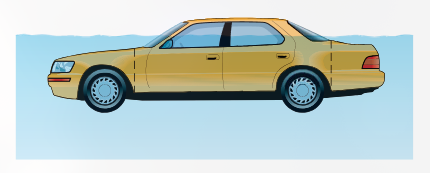
\includegraphics[width=0.45\linewidth]{images/47.png}
  \caption{Ilustrasi Mobil dalam Air nomor 47}
  \label{fig:car}
\end{figure}
 
\diketahui
\begin{align*}
m &= \SI{1800}{\kilo\gram}, &
V_{\text{penumpang}} &= \SI{5,00}{\metre\cubed}\\
V_{\text{mesin+roda depan}} &= \SI{0,750}{\metre\cubed}, &
V_{\text{roda belakang+tangki+bagasi}} &= \SI{0,800}{\metre\cubed}
\end{align*}
 
\ditanya\ (a) Volume mobil yang tercelup $V_{\text{tc}}$ saat mengapung; (b) volume air
$V_a$ di dalam mobil saat mobil tepat tenggelam.
 
\konsep\ Mobil setimbang bila gaya apung sama dengan berat total.
 
\penyelesaian
 
\textbf{(a)} Mobil mengapung dengan berat $mg$:
\begin{equation}
\rho_{\text{air}}\, g\, V_{\text{tc}} = m g
\ \Longrightarrow\
V_{\text{tc}} = \frac{m}{\rho_{\text{air}}} = \frac{\SI{1800}{\kilo\gram}}{\SI{1,00e3}{\kilo\gram\per\metre\cubed}} = \SI{1,80}{\metre\cubed}
\end{equation}
 
\textbf{(b)} Saat mobil tepat tenggelam, seluruh volume luarnya
\begin{equation}
V_{\text{total}} = \SI{5,00}{\metre\cubed} + \SI{0,750}{\metre\cubed} + \SI{0,800}{\metre\cubed} = \SI{6,55}{\metre\cubed}
\end{equation}
berada di dalam air, sehingga gaya apung $\rho_{\text{air}}\, g\, V_{\text{total}}$ sama dengan
berat mobil ditambah berat air yang masuk (massa udara diabaikan):
\begin{align}
\rho_{\text{air}}\, g\, V_{\text{total}} &= m g + \rho_{\text{air}}\, g\, V_a \\
V_a &= V_{\text{total}} - \frac{m}{\rho_{\text{air}}} = \SI{6,55}{\metre\cubed} - \SI{1,80}{\metre\cubed} = \SI{4,75}{\metre\cubed}
\end{align}
 
\begin{jawaban}
(a) $V_{\text{tc}} = \SI{1,80}{\metre\cubed}$.\\
(b) $V_a = \SI{4,75}{\metre\cubed}$.
\end{jawaban}
 
% =====================================================
\section*{Soal 48}
Gambar 16 memperlihatkan bola besi yang digantung dengan benang bermassa dapat diabaikan
dari sebuah silinder tegak yang mengapung sebagian tercelup di air. Silinder memiliki tinggi
$\SI{6,00}{\centi\metre}$, luas penampang atas dan bawah $\SI{12,0}{\centi\metre\squared}$, serta
massa jenis $\SI{0,30}{\gram\per\cubic\centi\metre}$, dan $\SI{2,00}{\centi\metre}$ dari
tingginya berada di atas permukaan air. Berapa jari-jari bola besi?

\begin{figure}[H]
  \centering
  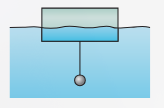
\includegraphics[width=0.45\linewidth]{images/48.png}
  \caption{Ilustrasi Bola Besi digantung Benang nomor 48}
  \label{fig:steel-ball}
\end{figure}
 
\diketahui\ (bola besi tercelup penuh, seperti pada Gambar 16)
\begin{align*}
h_s &= \SI{6,00}{\centi\metre}, &
A &= \SI{12,0}{\centi\metre\squared}, &
\rho_s &= \SI{0,30}{\gram\per\cubic\centi\metre}, &
h_{\text{atas}} &= \SI{2,00}{\centi\metre}\\
\rho_{\text{besi}} &= \SI{7,87}{\gram\per\cubic\centi\metre} \ \text{(asumsi, nilai besi seperti pada Soal 37 dan 45)}, &
\rho_{\text{air}} &= \SI{1,00}{\gram\per\cubic\centi\metre}
\end{align*}
 
\ditanya\ Jari-jari bola besi $r$.
 
\konsep\ Tinjau sistem silinder + bola. Berat total harus sama dengan gaya apung total:
gaya apung pada bagian silinder yang tercelup ditambah gaya apung pada bola.
\begin{equation*}
(m_s + m_b)\,g = \rho_{\text{air}}\,g\,(V_{s,\text{tc}} + V_b)
\end{equation*}
 
\penyelesaian
\begin{align}
V_s &= A h_s = (\num{12,0})(\num{6,00}) = \SI{72,0}{\centi\metre\cubed}, &
m_s &= \rho_s V_s = \SI{21,6}{\gram} \\
V_{s,\text{tc}} &= A\,(h_s - h_{\text{atas}}) = (\num{12,0})(\num{4,00}) = \SI{48,0}{\centi\metre\cubed}
\end{align}
Dengan $m_b = \rho_{\text{besi}} V_b$:
\begin{align}
m_s + \rho_{\text{besi}} V_b &= \rho_{\text{air}}\left(V_{s,\text{tc}} + V_b\right) \\
V_b\left(\rho_{\text{besi}} - \rho_{\text{air}}\right) &= \rho_{\text{air}} V_{s,\text{tc}} - m_s
 = \SI{48,0}{\gram} - \SI{21,6}{\gram} = \SI{26,4}{\gram} \\
V_b &= \frac{\SI{26,4}{\gram}}{(\num{7,87} - \num{1,00})\,\si{\gram\per\cubic\centi\metre}} = \SI{3,84}{\centi\metre\cubed}
\end{align}
Jari-jari bola:
\begin{equation}
r = \left(\frac{3 V_b}{4\pi}\right)^{1/3} = \left(\frac{3\,(\num{3,84})}{4\pi}\right)^{1/3}\si{\centi\metre} = \SI{0,972}{\centi\metre}
\end{equation}
 
\begin{jawaban}
$r \approx \SI{0,97}{\centi\metre}$.
\end{jawaban}
 
% =====================================================
\section*{Soal 49}
\textit{Efek kanal.} Gambar 17 memperlihatkan sebuah tongkang yang ditambatkan dan
membentang melintasi kanal sejauh $d = \SI{30}{\metre}$ serta masuk ke dalam air sedalam
$b = \SI{12}{\metre}$. Lebar kanal $D = \SI{55}{\metre}$, kedalaman air $H = \SI{14}{\metre}$,
dan kelajuan aliran air yang seragam $v_i = \SI{1,5}{\meter\per\second}$. Anggap aliran di
sekitar tongkang seragam. Saat air melewati haluan, permukaan air mengalami penurunan tajam
yang dikenal sebagai efek kanal. Jika kedalaman penurunan itu $h = \SI{0,80}{\metre}$,
berapa kelajuan air di sepanjang tongkang melalui penampang vertikal di (a) titik $a$ dan
(b) titik $b$?

\begin{figure}[H]
  \centering
  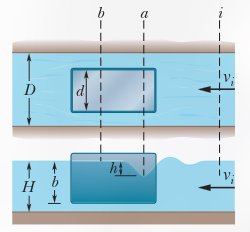
\includegraphics[width=0.45\linewidth]{images/49.png}
  \caption{Ilustrasi Tongkang Dilambatkan nomor 49}
  \label{fig:tongkang}
\end{figure}
 
\diketahui\ (dari Gambar 17)
\begin{align*}
D &= \SI{55}{\metre}, &
H &= \SI{14}{\metre}, &
d &= \SI{30}{\metre}, &
b &= \SI{12}{\metre}, &
h &= \SI{0,80}{\metre}, &
v_i &= \SI{1,5}{\meter\per\second}
\end{align*}
Pada titik $a$ permukaan air turun sedalam $h$; pada titik $b$ permukaan air kembali ke
ketinggian normal $H$. Tongkang menempati bagian penampang seluas $d\,b$ pada kedua titik.
 
\ditanya\ $v_a$ dan $v_b$.
 
\konsep\ Persamaan kontinuitas untuk fluida tak termampatkan: $A_i v_i = A_a v_a = A_b v_b$.
 
\penyelesaian
 
Luas penampang air yang dapat dilalui:
\begin{align}
A_i &= D H = (\SI{55}{\metre})(\SI{14}{\metre}) = \SI{770}{\metre\squared} \\
A_a &= D\,(H - h) - d b = (\num{55})(\num{13,2}) - (\num{30})(\num{12}) = \SI{366}{\metre\squared} \\
A_b &= D H - d b = \num{770} - \num{360} = \SI{410}{\metre\squared}
\end{align}
Kelajuan air:
\begin{align}
v_a &= v_i\,\frac{A_i}{A_a} = (\SI{1,5}{\meter\per\second})\frac{\SI{770}{\metre\squared}}{\SI{366}{\metre\squared}} = \SI{3,16}{\meter\per\second} \\
v_b &= v_i\,\frac{A_i}{A_b} = (\SI{1,5}{\meter\per\second})\frac{\SI{770}{\metre\squared}}{\SI{410}{\metre\squared}} = \SI{2,82}{\meter\per\second}
\end{align}
 
\begin{jawaban}
(a) $v_a \approx \SI{3,2}{\meter\per\second}$.\\
(b) $v_b \approx \SI{2,8}{\meter\per\second}$.
\end{jawaban}
 
% =====================================================
\section*{Soal 50}
Gambar 18 memperlihatkan dua bagian sistem pipa tua yang melewati sebuah bukit, dengan
jarak $d_A = d_B = \SI{30}{\metre}$ dan $D = \SI{110}{\metre}$. Di kedua sisi bukit, jari-jari
pipa $\SI{2,00}{\centi\metre}$, tetapi jari-jari pipa di dalam bukit tidak diketahui. Untuk
menentukannya, para insinyur pertama-tama memastikan air mengalir pada bagian kiri dan kanan
dengan kelajuan $\SI{2,50}{\meter\per\second}$. Kemudian mereka melepas zat pewarna di titik
$A$ dan mendapati bahwa pewarna tiba di titik $B$ dalam $\SI{88,8}{\second}$. Berapa jari-jari
rata-rata pipa di dalam bukit?

\begin{figure}[H]
  \centering
  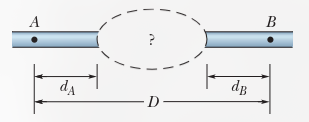
\includegraphics[width=0.45\linewidth]{images/50.png}
  \caption{Ilustrasi Sistem Pipa Melewati Bukit nomor 50}
  \label{fig:pipe-system}
\end{figure}
 
\diketahui\ (dari Gambar 18: $A$ dan $B$ berada pada pipa di luar bukit, dan $D$ adalah jarak total $A$ ke $B$)
\begin{align*}
d_A &= d_B = \SI{30}{\metre}, &
D &= \SI{110}{\metre}, &
r_o &= \SI{2,00}{\centi\metre}, &
v_o &= \SI{2,50}{\meter\per\second}, &
t &= \SI{88,8}{\second}
\end{align*}
 
\ditanya\ Jari-jari rata-rata pipa di dalam bukit, $r_h$.
 
\konsep\ Panjang pipa dalam bukit $L_h = D - d_A - d_B$. Waktu tempuh pewarna adalah jumlah
waktu di bagian luar (kelajuan $v_o$) dan bagian dalam bukit (kelajuan $v_h$). Kelajuan di
bukit diperoleh dari waktu, lalu persamaan kontinuitas memberi jari-jari.
 
\penyelesaian
\begin{align}
L_h &= D - d_A - d_B = \SI{110}{\metre} - \SI{60}{\metre} = \SI{50}{\metre} \\
t_{\text{luar}} &= \frac{d_A + d_B}{v_o} = \frac{\SI{60}{\metre}}{\SI{2,50}{\meter\per\second}} = \SI{24,0}{\second} \\
t_h &= t - t_{\text{luar}} = \SI{88,8}{\second} - \SI{24,0}{\second} = \SI{64,8}{\second} \\
v_h &= \frac{L_h}{t_h} = \frac{\SI{50}{\metre}}{\SI{64,8}{\second}} = \SI{0,772}{\meter\per\second}
\end{align}
Kontinuitas: $\pi r_o^2 v_o = \pi r_h^2 v_h$, sehingga
\begin{equation}
r_h = r_o\sqrt{\frac{v_o}{v_h}} = (\SI{2,00}{\centi\metre})\sqrt{\frac{\num{2,50}}{\num{0,772}}}
 = (\SI{2,00}{\centi\metre})(\num{1,80}) = \SI{3,60}{\centi\metre}
\end{equation}
 
\begin{jawaban}
$r_h \approx \SI{3,60}{\centi\metre}$.
\end{jawaban}

\section*{Soal 51}
Sebuah selang taman berdiameter dalam $\SI{1,9}{\centi\metre}$ disambungkan ke sebuah
penyiram halaman (diam) yang hanya berupa wadah dengan 24 lubang, masing-masing berdiameter
$\SI{0,13}{\centi\metre}$. Jika kelajuan air di dalam selang $\SI{0,91}{\meter\per\second}$,
berapa kelajuan air saat keluar dari lubang-lubang penyiram?
 
\diketahui
\begin{align*}
D &= \SI{1,9}{\centi\metre}, &
v_s &= \SI{0,91}{\meter\per\second}, &
N &= 24, &
d &= \SI{0,13}{\centi\metre}
\end{align*}
 
\ditanya\ Kelajuan air keluar dari tiap lubang, $v$.
 
\konsep\ Persamaan kontinuitas: debit air dalam selang sama dengan jumlah debit seluruh
lubang, $A_s v_s = N A_l v$. Karena luas lingkaran sebanding dengan kuadrat diameter,
$A_s/A_l = (D/d)^2$.
 
\penyelesaian
\begin{align}
v &= \frac{A_s}{N A_l}\,v_s = \frac{1}{N}\left(\frac{D}{d}\right)^2 v_s \\
  &= \frac{1}{24}\left(\frac{\SI{1,9}{\centi\metre}}{\SI{0,13}{\centi\metre}}\right)^2 (\SI{0,91}{\meter\per\second})
   = \frac{(\num{213,6})(\SI{0,91}{\meter\per\second})}{24} = \SI{8,1}{\meter\per\second}
\end{align}
 
\begin{jawaban}
$v \approx \SI{8,1}{\meter\per\second}$.
\end{jawaban}
 
% =====================================================
\section*{Soal 52}
Dua anak sungai bergabung membentuk sebuah sungai. Anak sungai pertama berlebar
$\SI{8,2}{\metre}$, dalam $\SI{3,4}{\metre}$, dengan kelajuan arus $\SI{2,3}{\meter\per\second}$.
Anak sungai kedua berlebar $\SI{6,8}{\metre}$ dan dalam $\SI{3,2}{\metre}$, mengalir pada
$\SI{2,6}{\meter\per\second}$. Jika sungai yang terbentuk berlebar $\SI{10,5}{\metre}$ dan
berkelajuan $\SI{2,9}{\meter\per\second}$, berapa kedalamannya?
 
\diketahui
\begin{align*}
w_1 &= \SI{8,2}{\metre}, & h_1 &= \SI{3,4}{\metre}, & v_1 &= \SI{2,3}{\meter\per\second}\\
w_2 &= \SI{6,8}{\metre}, & h_2 &= \SI{3,2}{\metre}, & v_2 &= \SI{2,6}{\meter\per\second}\\
w_3 &= \SI{10,5}{\metre}, & v_3 &= \SI{2,9}{\meter\per\second}
\end{align*}
 
\ditanya\ Kedalaman sungai, $h_3$.
 
\konsep\ Kontinuitas (debit volume kekal): $Q_1 + Q_2 = Q_3$ dengan $Q = w\,h\,v$.
 
\penyelesaian
\begin{align}
Q_1 &= (\num{8,2})(\num{3,4})(\num{2,3}) = \SI{64,1}{\metre\cubed\per\second} \\
Q_2 &= (\num{6,8})(\num{3,2})(\num{2,6}) = \SI{56,6}{\metre\cubed\per\second} \\
h_3 &= \frac{Q_1 + Q_2}{w_3 v_3} = \frac{\SI{120,7}{\metre\cubed\per\second}}{(\SI{10,5}{\metre})(\SI{2,9}{\meter\per\second})}
 = \SI{3,96}{\metre}
\end{align}
 
\begin{jawaban}
$h_3 \approx \SI{4,0}{\metre}$.
\end{jawaban}
 
% =====================================================
\section*{Soal 53}
Air dipompa keluar dari ruang bawah tanah yang banjir secara tetap dengan kelajuan
$\SI{5,0}{\meter\per\second}$ melalui selang berjari-jari $\SI{1,0}{\centi\metre}$, melewati
sebuah jendela yang $\SI{3,0}{\metre}$ di atas permukaan air. Berapa daya pompa?
 
\diketahui
\begin{align*}
v &= \SI{5,0}{\meter\per\second}, &
r &= \SI{1,0}{\centi\metre} = \SI{1,0e-2}{\metre}, &
h &= \SI{3,0}{\metre}
\end{align*}
 
\ditanya\ Daya pompa $P$.
 
\konsep\ Pompa menaikkan air setinggi $h$ dan memberinya energi kinetik. Dalam selang waktu
$\Delta t$, massa air yang dipindahkan $\Delta m = \rho A v\,\Delta t$. Daya adalah usaha per
satuan waktu (kelajuan air di permukaan genangan diabaikan, tekanan di kedua ujung sama
dengan tekanan atmosfer):
\begin{equation*}
P = \frac{\Delta m}{\Delta t}\left(\tfrac{1}{2}v^2 + g h\right)
\end{equation*}
 
\penyelesaian
\begin{align}
\frac{\Delta m}{\Delta t} &= \rho \pi r^2 v = (\num{1,00e3})\,\pi\,(\num{1,0e-2})^2(\num{5,0}) = \SI{1,57}{\kilo\gram\per\second} \\
P &= (\SI{1,57}{\kilo\gram\per\second})\left[\tfrac{1}{2}(\num{5,0})^2 + (\num{9,8})(\num{3,0})\right]\si{\joule\per\kilo\gram} \\
  &= (\num{1,57})(\num{12,5} + \num{29,4}) = \SI{66}{\watt}
\end{align}
 
\begin{jawaban}
$P \approx \SI{66}{\watt}$.
\end{jawaban}
 
% =====================================================
\section*{Soal 54}
Air yang mengalir melalui pipa berdiameter dalam $\SI{1,9}{\centi\metre}$ keluar melalui tiga
pipa berdiameter $\SI{1,3}{\centi\metre}$. (a) Jika debit di ketiga pipa kecil adalah
$\SI{26}{\litre\per\minute}$, $\SI{19}{\litre\per\minute}$, dan $\SI{11}{\litre\per\minute}$,
berapa debit di pipa $\SI{1,9}{\centi\metre}$? (b) Berapa perbandingan kelajuan di pipa
$\SI{1,9}{\centi\metre}$ terhadap kelajuan di pipa yang mengalirkan $\SI{26}{\litre\per\minute}$?
 
\diketahui
\begin{align*}
D &= \SI{1,9}{\centi\metre}, &
d &= \SI{1,3}{\centi\metre}, &
Q_1 &= \SI{26}{\litre\per\minute}, &
Q_2 &= \SI{19}{\litre\per\minute}, &
Q_3 &= \SI{11}{\litre\per\minute}
\end{align*}
 
\ditanya\ (a) $Q$ pada pipa besar; (b) $v_{D}/v_{1}$.
 
\konsep\ Kontinuitas: debit masuk $=$ jumlah debit keluar, dan $Q = A v$ dengan
$A \propto (\text{diameter})^2$.
 
\penyelesaian
 
\textbf{(a)}
\begin{equation}
Q = Q_1 + Q_2 + Q_3 = \SI{26}{\litre\per\minute} + \SI{19}{\litre\per\minute} + \SI{11}{\litre\per\minute} = \SI{56}{\litre\per\minute}
\end{equation}
 
\textbf{(b)} Kelajuan $v = Q/A$, sehingga
\begin{equation}
\frac{v_D}{v_1} = \frac{Q/A_D}{Q_1/A_d} = \frac{Q}{Q_1}\left(\frac{d}{D}\right)^2
 = \frac{\num{56}}{\num{26}}\left(\frac{\num{1,3}}{\num{1,9}}\right)^2 = (\num{2,15})(\num{0,468}) = \num{1,01}
\end{equation}
 
\begin{jawaban}
(a) $Q = \SI{56}{\litre\per\minute}$.\\
(b) $v_D/v_1 \approx \num{1,01}$.
\end{jawaban}
 
% =====================================================
\section*{Soal 55}
Berapa usaha yang dilakukan oleh tekanan dalam mendorong $\SI{1,4}{\metre\cubed}$ air
melalui pipa berdiameter dalam $\SI{13}{\milli\metre}$, jika selisih tekanan di kedua ujung
pipa $\SI{1,0}{\atm}$?
 
\diketahui
\begin{align*}
V &= \SI{1,4}{\metre\cubed}, &
\Delta p &= \SI{1,0}{\atm} = \SI{1,013e5}{\pascal}, &
d &= \SI{13}{\milli\metre}
\end{align*}
 
\ditanya\ Usaha oleh tekanan, $W$.
 
\konsep\ Usaha oleh gaya tekan pada fluida yang bergerak sejauh $\Delta x$ dalam pipa
berpenampang $A$ adalah $W = (\Delta p\,A)\,\Delta x = \Delta p\,V$, sehingga tidak bergantung
pada diameter pipa.
 
\penyelesaian
\begin{equation}
W = \Delta p\, V = (\SI{1,013e5}{\pascal})(\SI{1,4}{\metre\cubed}) = \SI{1,4e5}{\joule}
\end{equation}
 
\begin{jawaban}
$W \approx \SI{1,4e5}{\joule}$ (diameter pipa tidak berpengaruh pada hasil).
\end{jawaban}

\section*{Soal 56}
Misalkan dua tangki, 1 dan 2, masing-masing dengan bukaan besar di atas, berisi cairan yang
berbeda. Sebuah lubang kecil dibuat di sisi tiap tangki pada kedalaman $h$ yang sama di bawah
permukaan cairan, tetapi lubang pada tangki 1 memiliki luas penampang setengah dari luas
lubang pada tangki 2. (a) Berapa perbandingan massa jenis $\rho_1/\rho_2$ jika laju aliran
massa kedua lubang sama? (b) Berapa perbandingan laju aliran volume $R_{V1}/R_{V2}$?
(c) Pada suatu saat, cairan di tangki 1 berada $\SI{12,0}{\centi\metre}$ di atas lubang. Jika
kedua tangki harus memiliki laju aliran volume yang sama, berapa tinggi cairan di atas lubang
pada tangki 2 saat itu?
 
\diketahui
\begin{align*}
A_1 &= \tfrac{1}{2}A_2, &
h_1' &= \SI{12,0}{\centi\metre} \ \text{(untuk bagian (c))}
\end{align*}
 
\ditanya\ (a) $\rho_1/\rho_2$; (b) $R_{V1}/R_{V2}$; (c) $h_2'$.
 
\konsep\ Teorema Torricelli: kelajuan semburan dari lubang pada kedalaman $h$ adalah
$v = \sqrt{2gh}$ (tidak bergantung pada massa jenis). Laju aliran volume $R_V = A v$ dan laju
aliran massa $R_m = \rho A v$.
 
\penyelesaian
 
\textbf{(a)} Kedua lubang berada pada kedalaman sama, sehingga $v_1 = v_2$. Laju aliran massa sama:
\begin{equation}
\rho_1 A_1 v = \rho_2 A_2 v
\ \Longrightarrow\
\frac{\rho_1}{\rho_2} = \frac{A_2}{A_1} = 2
\end{equation}
 
\textbf{(b)}
\begin{equation}
\frac{R_{V1}}{R_{V2}} = \frac{A_1 v}{A_2 v} = \frac{A_1}{A_2} = \frac{1}{2}
\end{equation}
 
\textbf{(c)} Laju aliran volume sama: $A_1 v_1 = A_2 v_2$, sehingga
$v_2 = v_1 A_1/A_2 = v_1/2$. Dengan $v = \sqrt{2gh}$:
\begin{equation}
\sqrt{2 g h_2'} = \tfrac{1}{2}\sqrt{2 g h_1'}
\ \Longrightarrow\
h_2' = \frac{h_1'}{4} = \frac{\SI{12,0}{\centi\metre}}{4} = \SI{3,00}{\centi\metre}
\end{equation}
 
\begin{jawaban}
(a) $\rho_1/\rho_2 = 2$.\\
(b) $R_{V1}/R_{V2} = \tfrac{1}{2}$.\\
(c) $h_2' = \SI{3,00}{\centi\metre}$.
\end{jawaban}
 
% =====================================================
\section*{Soal 57}
Sebuah tangki silinder berdiameter besar diisi air sedalam $D = \SI{0,30}{\metre}$. Sebuah
lubang berluas penampang $A = \SI{6,5}{\centi\metre\squared}$ di dasar tangki memungkinkan
air mengalir keluar. (a) Berapa laju pengeluaran air dalam meter kubik per detik? (b) Pada
jarak berapa di bawah dasar tangki luas penampang aliran air sama dengan setengah luas lubang?
 
\diketahui
\begin{align*}
D &= \SI{0,30}{\metre}, &
A &= \SI{6,5}{\centi\metre\squared} = \SI{6,5e-4}{\metre\squared}
\end{align*}
 
\ditanya\ (a) $R_V$; (b) jarak $y$ di bawah dasar tangki.
 
\konsep\ Karena tangki berdiameter besar, kelajuan permukaan atas dapat diabaikan, dan
tekanan di permukaan serta di aliran keluar sama dengan tekanan atmosfer. Bernoulli
(Torricelli) memberi $v_0 = \sqrt{2 g D}$. Setelah keluar, air jatuh bebas dan
kontinuitas $A_0 v_0 = A v$ berlaku.
 
\penyelesaian
 
\textbf{(a)}
\begin{align}
v_0 &= \sqrt{2 g D} = \sqrt{2(\num{9,8})(\num{0,30})} = \SI{2,42}{\meter\per\second} \\
R_V &= A v_0 = (\SI{6,5e-4}{\metre\squared})(\SI{2,42}{\meter\per\second}) = \SI{1,6e-3}{\metre\cubed\per\second}
\end{align}
 
\textbf{(b)} Luas aliran menjadi $A/2$ sehingga kelajuannya $v = 2 v_0$ (kontinuitas).
Untuk jatuh bebas sejauh $y$:
\begin{align}
v^2 &= v_0^2 + 2 g y \ \Longrightarrow\ (2v_0)^2 = v_0^2 + 2 g y \\
y &= \frac{3 v_0^2}{2 g} = \frac{3\,(2 g D)}{2 g} = 3D = 3(\SI{0,30}{\metre}) = \SI{0,90}{\metre}
\end{align}
 
\begin{jawaban}
(a) $R_V \approx \SI{1,6e-3}{\metre\cubed\per\second}$.\\
(b) $y = \SI{0,90}{\metre}$ di bawah dasar tangki.
\end{jawaban}
 
% =====================================================
\section*{Soal 58}
Pipa masuk (\textit{intake}) pada Gambar 19 memiliki luas penampang $\SI{0,74}{\metre\squared}$
dan air mengalir dengan kelajuan $\SI{0,40}{\meter\per\second}$. Pada keluaran (\textit{outlet}),
yang berada $D = \SI{180}{\metre}$ di bawah pipa masuk, luas penampang lebih kecil daripada pipa
masuk dan air mengalir keluar dengan kelajuan $\SI{9,5}{\meter\per\second}$ menuju peralatan.
Berapa selisih tekanan antara pipa masuk dan keluaran?
 
\begin{figure}[H]
  \centering
  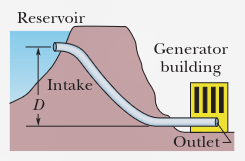
\includegraphics[width=0.45\linewidth]{images/58.png}
  \caption{Ilustrasi Pipa Penampang nomor 58}
  \label{fig:pipe}
\end{figure}
 
\diketahui
\begin{align*}
A_{\text{in}} &= \SI{0,74}{\metre\squared}, &
v_{\text{in}} &= \SI{0,40}{\meter\per\second}, &
v_{\text{out}} &= \SI{9,5}{\meter\per\second}, &
D &= \SI{180}{\metre}
\end{align*}
 
\ditanya\ $\Delta p = p_{\text{out}} - p_{\text{in}}$.
 
\konsep\ Persamaan Bernoulli antara pipa masuk (ketinggian lebih tinggi sebesar $D$)
dan keluaran:
\begin{equation*}
p_{\text{in}} + \tfrac{1}{2}\rho v_{\text{in}}^2 + \rho g D = p_{\text{out}} + \tfrac{1}{2}\rho v_{\text{out}}^2
\end{equation*}
 
\penyelesaian
\begin{align}
\Delta p &= p_{\text{out}} - p_{\text{in}} = \rho g D + \tfrac{1}{2}\rho\left(v_{\text{in}}^2 - v_{\text{out}}^2\right) \\
 &= (\num{1,00e3})(\num{9,8})(\num{180}) + \tfrac{1}{2}(\num{1,00e3})\left[(\num{0,40})^2 - (\num{9,5})^2\right] \\
 &= \SI{1,764e6}{\pascal} - \SI{4,5e4}{\pascal} = \SI{1,72e6}{\pascal}
\end{align}
 
\begin{jawaban}
$p_{\text{out}} - p_{\text{in}} \approx \SI{1,7e6}{\pascal}$ (tekanan di keluaran lebih besar).
\end{jawaban}
 
% =====================================================
\section*{Soal 59}
Air bergerak dengan kelajuan $\SI{5,0}{\meter\per\second}$ melalui pipa berluas penampang
$\SI{4,0}{\centi\metre\squared}$. Air turun perlahan sejauh $\SI{10}{\metre}$ sementara luas
penampang pipa membesar menjadi $\SI{8,0}{\centi\metre\squared}$. (a) Berapa kelajuan air di
tingkat yang lebih rendah? (b) Jika tekanan di tingkat atas $\SI{1,5e5}{\pascal}$, berapa
tekanan di tingkat bawah?
 
\diketahui
\begin{align*}
v_1 &= \SI{5,0}{\meter\per\second}, &
A_1 &= \SI{4,0}{\centi\metre\squared}, &
A_2 &= \SI{8,0}{\centi\metre\squared}, &
\Delta y &= \SI{10}{\metre}, &
p_1 &= \SI{1,5e5}{\pascal}
\end{align*}
 
\ditanya\ (a) $v_2$; (b) $p_2$.
 
\konsep\ Kontinuitas $A_1 v_1 = A_2 v_2$ dan Bernoulli
$p_1 + \tfrac{1}{2}\rho v_1^2 + \rho g y_1 = p_2 + \tfrac{1}{2}\rho v_2^2 + \rho g y_2$
dengan $y_1 - y_2 = \SI{10}{\metre}$.
 
\penyelesaian
 
\textbf{(a)}
\begin{equation}
v_2 = v_1\,\frac{A_1}{A_2} = (\SI{5,0}{\meter\per\second})\frac{\num{4,0}}{\num{8,0}} = \SI{2,5}{\meter\per\second}
\end{equation}
 
\textbf{(b)}
\begin{align}
p_2 &= p_1 + \tfrac{1}{2}\rho\left(v_1^2 - v_2^2\right) + \rho g\,(y_1 - y_2) \\
 &= \SI{1,5e5}{\pascal} + \tfrac{1}{2}(\num{1,00e3})\left[(\num{5,0})^2 - (\num{2,5})^2\right] + (\num{1,00e3})(\num{9,8})(\num{10}) \\
 &= \SI{1,5e5}{\pascal} + \SI{9,4e3}{\pascal} + \SI{9,8e4}{\pascal} = \SI{2,6e5}{\pascal}
\end{align}
 
\begin{jawaban}
(a) $v_2 = \SI{2,5}{\meter\per\second}$.\\
(b) $p_2 \approx \SI{2,6e5}{\pascal}$.
\end{jawaban}
 
% =====================================================
\section*{Soal 60}
Model torpedo kadang diuji dalam pipa horizontal berisi air mengalir, seperti terowongan
angin untuk menguji model pesawat. Misalkan pipa melingkar berdiameter dalam
$\SI{25,0}{\centi\metre}$ dan model torpedo diletakkan sejajar sumbu panjang pipa. Model
berdiameter $\SI{5,00}{\centi\metre}$ dan diuji dengan air yang mengalir melewatinya pada
$\SI{2,50}{\meter\per\second}$. (a) Dengan kelajuan berapa air harus mengalir di bagian pipa
yang tidak dipersempit model? (b) Berapa selisih tekanan antara bagian pipa yang
dipersempit dan yang tidak dipersempit?
 
\diketahui
\begin{align*}
D &= \SI{25,0}{\centi\metre}, &
d &= \SI{5,00}{\centi\metre}, &
v_c &= \SI{2,50}{\meter\per\second}
\end{align*}
 
\ditanya\ (a) $v_u$ (kelajuan di bagian tak terpersempit); (b) $\Delta p$.
 
\konsep\ Luas penampang bagian bebas pipa di sekitar model (bagian terpersempit):
$A_c = \tfrac{\pi}{4}\left(D^2 - d^2\right)$, sedangkan bagian tak terpersempit
$A_u = \tfrac{\pi}{4}D^2$. Kontinuitas $A_u v_u = A_c v_c$ dan Bernoulli (pipa horizontal)
$p_u + \tfrac{1}{2}\rho v_u^2 = p_c + \tfrac{1}{2}\rho v_c^2$.
 
\penyelesaian
 
\textbf{(a)}
\begin{equation}
v_u = v_c\,\frac{A_c}{A_u} = v_c\,\frac{D^2 - d^2}{D^2}
 = (\SI{2,50}{\meter\per\second})\frac{\num{625} - \num{25}}{\num{625}} = \SI{2,40}{\meter\per\second}
\end{equation}
 
\textbf{(b)}
\begin{align}
p_u - p_c &= \tfrac{1}{2}\rho\left(v_c^2 - v_u^2\right)
 = \tfrac{1}{2}(\num{1,00e3})\left[(\num{2,50})^2 - (\num{2,40})^2\right] \\
 &= \tfrac{1}{2}(\num{1,00e3})(\num{0,490}) = \SI{245}{\pascal}
\end{align}
 
\begin{jawaban}
(a) $v_u = \SI{2,40}{\meter\per\second}$.\\
(b) $\Delta p = \SI{245}{\pascal}$ (tekanan di bagian terpersempit lebih kecil).
\end{jawaban}

\section*{Soal 61}
Sebuah pipa air berdiameter dalam $\SI{2,5}{\centi\metre}$ membawa air ke ruang bawah tanah
sebuah rumah dengan kelajuan $\SI{0,90}{\meter\per\second}$ dan tekanan $\SI{170}{\kilo\pascal}$.
Jika pipa menyempit menjadi $\SI{1,2}{\centi\metre}$ dan naik ke lantai dua yang
$\SI{7,6}{\metre}$ di atas titik masuk, berapa (a) kelajuan dan (b) tekanan air di lantai dua?

\diketahui
\begin{align*}
d_1 &= \SI{2,5}{\centi\metre}, &
v_1 &= \SI{0,90}{\meter\per\second}, &
p_1 &= \SI{170}{\kilo\pascal}\\
d_2 &= \SI{1,2}{\centi\metre}, &
h &= \SI{7,6}{\metre}
\end{align*}

\ditanya\ (a) $v_2$; (b) $p_2$.

\konsep\ Kontinuitas $A_1 v_1 = A_2 v_2$ dengan $A \propto d^2$, dan Bernoulli
$p_1 + \tfrac{1}{2}\rho v_1^2 = p_2 + \tfrac{1}{2}\rho v_2^2 + \rho g h$.

\penyelesaian

\textbf{(a)}
\begin{equation}
v_2 = v_1\left(\frac{d_1}{d_2}\right)^2 = (\SI{0,90}{\meter\per\second})\left(\frac{\num{2,5}}{\num{1,2}}\right)^2 = \SI{3,9}{\meter\per\second}
\end{equation}

\textbf{(b)}
\begin{align}
p_2 &= p_1 + \tfrac{1}{2}\rho\left(v_1^2 - v_2^2\right) - \rho g h \\
 &= \SI{1,70e5}{\pascal} + \tfrac{1}{2}(\num{1,00e3})\left[(\num{0,90})^2 - (\num{3,91})^2\right] - (\num{1,00e3})(\num{9,8})(\num{7,6}) \\
 &= \SI{1,70e5}{\pascal} - \SI{7,2e3}{\pascal} - \SI{7,45e4}{\pascal} = \SI{8,8e4}{\pascal}
\end{align}

\begin{jawaban}
(a) $v_2 \approx \SI{3,9}{\meter\per\second}$.\\
(b) $p_2 \approx \SI{8,8e4}{\pascal}$ ($\SI{88}{\kilo\pascal}$).
\end{jawaban}

% =====================================================
\section*{Soal 62}
Sebuah \textit{tabung pitot} (Gambar 14-48) dipakai untuk menentukan kelajuan udara sebuah
pesawat. Alat ini terdiri atas tabung luar dengan sejumlah lubang kecil $B$ (empat lubang
ditunjukkan) yang memungkinkan udara masuk ke dalam tabung; tabung itu terhubung ke satu
lengan pipa-U. Lengan lain pipa-U terhubung ke lubang $A$ di ujung depan alat, yang menghadap
ke arah gerak pesawat. Di $A$ udara menjadi diam sehingga $v_A = 0$. Namun di $B$, kelajuan
udara dianggap sama dengan kelajuan udara $v$ pesawat. (a) Gunakan persamaan Bernoulli untuk
menunjukkan bahwa
\begin{equation*}
v = \sqrt{\frac{2\rho g h}{\rho_{\text{udara}}}}
\end{equation*}
dengan $\rho$ massa jenis cairan dalam pipa-U dan $h$ selisih tinggi permukaan cairan.
(b) Misalkan tabung berisi alkohol dan selisih tinggi $h = \SI{26,0}{\centi\metre}$. Berapa
kelajuan pesawat relatif terhadap udara? Massa jenis udara $\SI{1,03}{\kilo\gram\per\metre\cubed}$
dan alkohol $\SI{810}{\kilo\gram\per\metre\cubed}$.

\begin{figure}[H]
  \centering
  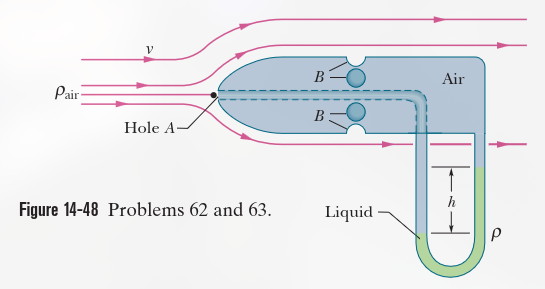
\includegraphics[width=0.45\linewidth]{images/62.png}
  \caption{Ilustrasi Tabung Pitot nomor 62 (juga dipakai pada Soal 63)}
  \label{fig:pitot-tube}
\end{figure}

\diketahui
\begin{align*}
\rho_{\text{alkohol}} &= \SI{810}{\kilo\gram\per\metre\cubed}, &
\rho_{\text{udara}} &= \SI{1,03}{\kilo\gram\per\metre\cubed}, &
h &= \SI{26,0}{\centi\metre} = \SI{0,260}{\metre}
\end{align*}

\ditanya\ (a) Pembuktian rumus $v$; (b) nilai $v$.

\konsep\ Titik $A$ (kelajuan nol) dan titik $B$ (kelajuan $v$) berada pada ketinggian yang
sama. Selisih tekanan di antara keduanya ditunjukkan oleh selisih tinggi cairan dalam pipa-U:
$p_A - p_B = \rho g h$.

\penyelesaian

\textbf{(a)} Bernoulli antara $A$ dan $B$:
\begin{align}
p_A + \tfrac{1}{2}\rho_{\text{udara}}(0)^2 &= p_B + \tfrac{1}{2}\rho_{\text{udara}}\, v^2 \\
p_A - p_B &= \tfrac{1}{2}\rho_{\text{udara}}\, v^2
\end{align}
Karena $p_A - p_B = \rho g h$,
\begin{equation}
\rho g h = \tfrac{1}{2}\rho_{\text{udara}}\, v^2
\ \Longrightarrow\
v = \sqrt{\frac{2\rho g h}{\rho_{\text{udara}}}} \qquad \blacksquare
\end{equation}

\textbf{(b)}
\begin{equation}
v = \sqrt{\frac{2(\num{810})(\num{9,8})(\num{0,260})}{\num{1,03}}} = \SI{63,3}{\meter\per\second}
\end{equation}

\begin{jawaban}
(a) $v = \sqrt{2\rho g h/\rho_{\text{udara}}}$ (terbukti).\\
(b) $v \approx \SI{63,3}{\meter\per\second}$.
\end{jawaban}

% =====================================================
\section*{Soal 63}
Sebuah tabung pitot (lihat Soal 62 dan gambarnya) pada pesawat berketinggian tinggi mengukur
selisih tekanan $\SI{180}{\pascal}$. Berapa kelajuan udara pesawat jika massa jenis udara
$\SI{0,031}{\kilo\gram\per\metre\cubed}$?

\diketahui
\begin{align*}
\Delta p &= \SI{180}{\pascal}, &
\rho_{\text{udara}} &= \SI{0,031}{\kilo\gram\per\metre\cubed}
\end{align*}

\ditanya\ Kelajuan udara $v$.

\konsep\ Dari Soal 62, selisih tekanan antara titik stagnasi dan titik aliran bebas adalah
$\Delta p = \tfrac{1}{2}\rho_{\text{udara}}\, v^2$.

\penyelesaian
\begin{equation}
v = \sqrt{\frac{2\,\Delta p}{\rho_{\text{udara}}}} = \sqrt{\frac{2(\num{180})}{\num{0,031}}} = \SI{1,1e2}{\meter\per\second}
\end{equation}

\begin{jawaban}
$v \approx \SI{1,1e2}{\meter\per\second}$ (tepatnya $\SI{108}{\meter\per\second}$).
\end{jawaban}

% =====================================================
\section*{Soal 64}
Pada Gambar 14-49, air mengalir melalui pipa horizontal lalu keluar ke atmosfer dengan
kelajuan $v_1 = \SI{15}{\meter\per\second}$. Diameter bagian pipa kiri dan kanan berturut-turut
$\SI{5,0}{\centi\metre}$ dan $\SI{3,0}{\centi\metre}$. (a) Berapa volume air yang mengalir
ke atmosfer selama $\SI{10}{\minute}$? Pada bagian kiri pipa, berapa (b) kelajuan $v_2$ dan
(c) tekanan gauge?

\begin{figure}[H]
  \centering
  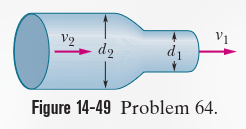
\includegraphics[width=0.45\linewidth]{images/64.png}
  \caption{Ilustrasi Aliran Air pada Pipa yang Menyempit nomor 64}
  \label{fig:pipa-menyempit}
\end{figure}

\diketahui
\begin{align*}
v_1 &= \SI{15}{\meter\per\second}, &
d_1 &= \SI{3,0}{\centi\metre}\ (\text{kanan}), &
d_2 &= \SI{5,0}{\centi\metre}\ (\text{kiri}), &
t &= \SI{10}{\minute} = \SI{600}{\second}
\end{align*}

\ditanya\ (a) $V$; (b) $v_2$; (c) $p_{g,2}$.

\konsep\ Debit $Q = A_1 v_1$; kontinuitas $A_1 v_1 = A_2 v_2$; Bernoulli untuk pipa horizontal
dengan tekanan di ujung keluar sama dengan tekanan atmosfer ($p_{g,1} = 0$).

\penyelesaian

\textbf{(a)}
\begin{align}
A_1 &= \pi\left(\frac{d_1}{2}\right)^2 = \pi(\SI{1,5e-2}{\metre})^2 = \SI{7,07e-4}{\metre\squared} \\
V &= A_1 v_1\, t = (\SI{7,07e-4}{\metre\squared})(\SI{15}{\meter\per\second})(\SI{600}{\second}) = \SI{6,4}{\metre\cubed}
\end{align}

\textbf{(b)}
\begin{equation}
v_2 = v_1\left(\frac{d_1}{d_2}\right)^2 = (\SI{15}{\meter\per\second})\left(\frac{\num{3,0}}{\num{5,0}}\right)^2 = \SI{5,4}{\meter\per\second}
\end{equation}

\textbf{(c)}
\begin{align}
p_{g,2} &= p_2 - p_0 = \tfrac{1}{2}\rho\left(v_1^2 - v_2^2\right) \\
 &= \tfrac{1}{2}(\num{1,00e3})\left[(\num{15})^2 - (\num{5,4})^2\right] = \SI{9,8e4}{\pascal}
\end{align}

\begin{jawaban}
(a) $V \approx \SI{6,4}{\metre\cubed}$.\\
(b) $v_2 \approx \SI{5,4}{\meter\per\second}$.\\
(c) $p_{g,2} \approx \SI{9,8e4}{\pascal}$.
\end{jawaban}

% =====================================================
\section*{Soal 65}
Sebuah \textit{venturimeter} dipakai untuk mengukur kelajuan aliran fluida dalam pipa. Alat ini
dipasang di antara dua bagian pipa (Gambar 14-50); luas penampang $A$ pada pintu masuk dan
keluar alat sama dengan luas penampang pipa. Di antara pintu masuk dan keluar, fluida mengalir
dari pipa dengan kelajuan $V$ lalu melalui ``leher'' sempit berluas penampang $a$ dengan
kelajuan $v$. Sebuah manometer menghubungkan bagian lebar dengan bagian sempit. Perubahan
kelajuan fluida disertai perubahan tekanan $\Delta p$ (tekanan di leher dikurangi tekanan di
pipa), yang menyebabkan selisih tinggi $h$ cairan pada kedua lengan manometer. (a) Dengan
Bernoulli dan persamaan kontinuitas pada titik 1 dan 2, tunjukkan bahwa
\begin{equation*}
V = \sqrt{\frac{2a^2\,\Delta p}{\rho\,(a^2 - A^2)}}
\end{equation*}
dengan $\rho$ massa jenis fluida. (b) Misalkan fluida adalah air tawar, luas penampang pipa
$\SI{64}{\centi\metre\squared}$ dan leher $\SI{32}{\centi\metre\squared}$, tekanan di pipa
$\SI{55}{\kilo\pascal}$ dan di leher $\SI{41}{\kilo\pascal}$. Berapa laju aliran air dalam
meter kubik per detik?

\begin{figure}[H]
  \centering
  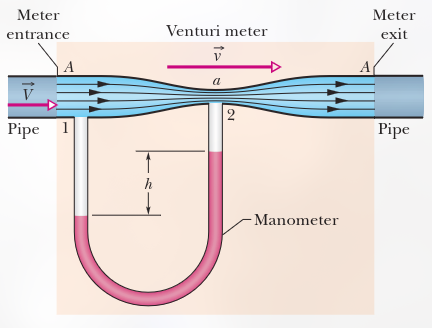
\includegraphics[width=0.45\linewidth]{images/65.png}
  \caption{Ilustrasi Venturimeter nomor 65 (juga dipakai pada Soal 66)}
  \label{fig:venturimeter}
\end{figure}

\diketahui
\begin{align*}
A &= \SI{64}{\centi\metre\squared} = \SI{6,4e-3}{\metre\squared}, &
a &= \SI{32}{\centi\metre\squared} = \SI{3,2e-3}{\metre\squared}\\
p_1 &= \SI{55}{\kilo\pascal}, &
p_2 &= \SI{41}{\kilo\pascal}, &
\rho &= \SI{1,00e3}{\kilo\gram\per\metre\cubed}
\end{align*}

\ditanya\ (a) Pembuktian rumus $V$; (b) laju aliran volume $R_V = A V$.

\konsep\ Titik 1 (pipa, kelajuan $V$, tekanan $p_1$) dan titik 2 (leher, kelajuan $v$,
tekanan $p_2$) berada pada ketinggian sama. Gunakan kontinuitas $A V = a v$ dan Bernoulli.

\penyelesaian

\textbf{(a)} Dari kontinuitas, $v = (A/a)\,V$. Bernoulli:
\begin{align}
p_1 + \tfrac{1}{2}\rho V^2 &= p_2 + \tfrac{1}{2}\rho v^2 \\
\Delta p = p_2 - p_1 &= \tfrac{1}{2}\rho\left(V^2 - v^2\right)
 = \tfrac{1}{2}\rho V^2\left(1 - \frac{A^2}{a^2}\right) = \frac{\rho V^2\,(a^2 - A^2)}{2a^2}
\end{align}
Menyelesaikan untuk $V$:
\begin{equation}
V = \sqrt{\frac{2a^2\,\Delta p}{\rho\,(a^2 - A^2)}} \qquad \blacksquare
\end{equation}
(Karena $a < A$, baik $\Delta p$ maupun $a^2 - A^2$ bernilai negatif sehingga $V^2 > 0$.)

\textbf{(b)}
\begin{align}
\Delta p &= \SI{41}{\kilo\pascal} - \SI{55}{\kilo\pascal} = -\SI{1,4e4}{\pascal} \\
V &= \sqrt{\frac{2(\SI{3,2e-3}{\metre\squared})^2(-\SI{1,4e4}{\pascal})}{(\SI{1,00e3}{\kilo\gram\per\metre\cubed})\left[(\SI{3,2e-3}{\metre\squared})^2 - (\SI{6,4e-3}{\metre\squared})^2\right]}}
 = \SI{3,06}{\meter\per\second} \\
R_V &= A V = (\SI{6,4e-3}{\metre\squared})(\SI{3,06}{\meter\per\second}) = \SI{2,0e-2}{\metre\cubed\per\second}
\end{align}

\begin{jawaban}
(a) $V = \sqrt{2a^2\Delta p/[\rho(a^2 - A^2)]}$ (terbukti).\\
(b) $R_V \approx \SI{2,0e-2}{\metre\cubed\per\second}$.
\end{jawaban}

\section*{Soal 66}
Tinjau tabung venturi pada Soal 65 dan Gambar 14-50 tanpa manometer. Misalkan $A$ sama
dengan $5a$. Tekanan $p_1$ di $A$ adalah $\SI{2,0}{\atm}$. Hitung (a) kelajuan $V$ di $A$ dan
(b) kelajuan $v$ di $a$ yang membuat tekanan $p_2$ di $a$ sama dengan nol. (c) Hitung laju
aliran volume yang bersesuaian jika diameter di $A$ adalah $\SI{5,0}{\centi\metre}$. Gejala
yang terjadi di $a$ ketika $p_2$ turun hingga hampir nol dikenal sebagai \textit{kavitasi}:
air menguap menjadi gelembung-gelembung kecil.

\diketahui
\begin{align*}
A &= 5a, &
p_1 &= \SI{2,0}{\atm} = \SI{2,03e5}{\pascal}, &
p_2 &= 0, &
d_A &= \SI{5,0}{\centi\metre}, &
\rho &= \SI{1,00e3}{\kilo\gram\per\metre\cubed}
\end{align*}

\ditanya\ (a) $V$; (b) $v$; (c) $R_V$.

\konsep\ Kontinuitas $A V = a v$ memberi $v = (A/a)\,V = 5V$. Bernoulli pada
ketinggian yang sama:
$p_1 + \tfrac{1}{2}\rho V^2 = p_2 + \tfrac{1}{2}\rho v^2$.

\penyelesaian

\textbf{(a)} Dengan $p_2 = 0$ dan $v = 5V$:
\begin{align}
p_1 &= \tfrac{1}{2}\rho\left[(5V)^2 - V^2\right] = 12\,\rho V^2 \\
V &= \sqrt{\frac{p_1}{12\rho}} = \sqrt{\frac{\SI{2,03e5}{\pascal}}{12(\SI{1,00e3}{\kilo\gram\per\metre\cubed})}} = \SI{4,1}{\meter\per\second}
\end{align}

\textbf{(b)}
\begin{equation}
v = 5V = 5(\SI{4,11}{\meter\per\second}) = \SI{21}{\meter\per\second}
\end{equation}

\textbf{(c)}
\begin{equation}
R_V = A V = \pi\left(\SI{2,5e-2}{\metre}\right)^2(\SI{4,11}{\meter\per\second}) = \SI{8,1e-3}{\metre\cubed\per\second}
\end{equation}

\begin{jawaban}
(a) $V \approx \SI{4,1}{\meter\per\second}$.\\
(b) $v \approx \SI{21}{\meter\per\second}$.\\
(c) $R_V \approx \SI{8,1e-3}{\metre\cubed\per\second}$.
\end{jawaban}

% =====================================================
\section*{Soal 67}
Pada Gambar 14-51, air tawar di belakang bendungan waduk memiliki kedalaman
$D = \SI{15}{\metre}$. Sebuah pipa horizontal berdiameter $\SI{4,0}{\centi\metre}$ menembus
bendungan pada kedalaman $d = \SI{6,0}{\metre}$. Sebuah sumbat menutup bukaan pipa. (a) Cari
besar gaya gesek antara sumbat dan dinding pipa. (b) Sumbat dilepas. Berapa volume air yang
keluar dari pipa dalam $\SI{3,0}{\hour}$?

\begin{figure}[H]
  \centering
  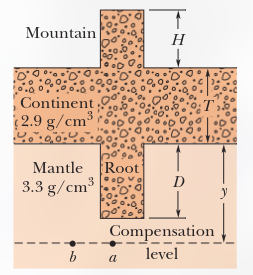
\includegraphics[width=0.45\linewidth]{images/23.png}
  \caption{Ilustrasi Pipa pada Bendungan Waduk nomor 67}
  \label{fig:bendungan-pipa}
\end{figure}

\diketahui
\begin{align*}
D &= \SI{15}{\metre}, &
d &= \SI{6,0}{\metre}, &
d_{\text{pipa}} &= \SI{4,0}{\centi\metre}\ (r = \SI{2,0e-2}{\metre}), &
t &= \SI{3,0}{\hour} = \SI{1,08e4}{\second}
\end{align*}

\ditanya\ (a) $f$; (b) $V$.

\konsep\ (a) Sumbat setimbang: gaya gesek menahan gaya akibat tekanan gauge air pada
kedalaman $d$ (tekanan atmosfer bekerja pada kedua sisi sumbat dan saling meniadakan).
(b) Waduk berukuran besar sehingga kedalaman dianggap tetap; Torricelli memberi kelajuan
semburan $v = \sqrt{2 g d}$.

\penyelesaian

\textbf{(a)}
\begin{align}
A &= \pi r^2 = \pi (\SI{2,0e-2}{\metre})^2 = \SI{1,26e-3}{\metre\squared} \\
f &= \rho g d\, A = (\num{1,00e3})(\num{9,8})(\num{6,0})(\SI{1,26e-3}{\metre\squared}) = \SI{74}{\newton}
\end{align}

\textbf{(b)}
\begin{align}
v &= \sqrt{2 g d} = \sqrt{2(\num{9,8})(\num{6,0})} = \SI{10,8}{\meter\per\second} \\
V &= A v\, t = (\SI{1,26e-3}{\metre\squared})(\SI{10,8}{\meter\per\second})(\SI{1,08e4}{\second}) = \SI{1,5e2}{\metre\cubed}
\end{align}

\begin{jawaban}
(a) $f \approx \SI{74}{\newton}$.\\
(b) $V \approx \SI{1,5e2}{\metre\cubed}$.
\end{jawaban}

% =====================================================
\section*{Soal 68}
Air tawar mengalir horizontal dari bagian pipa 1 berluas penampang $A_1$ ke bagian pipa 2
berluas penampang $A_2$. Gambar 14-52 memberikan plot selisih tekanan $p_2 - p_1$ terhadap
kebalikan kuadrat luas, $A_1^{-2}$, yang diharapkan untuk laju aliran volume tertentu jika
aliran air laminar dalam semua keadaan. Skala sumbu vertikal ditentukan oleh
$\Delta p_s = \SI{300}{\kilo\newton\per\metre\squared}$. Untuk kondisi pada gambar, berapa
(a) $A_2$ dan (b) laju aliran volume?

\begin{figure}[H]
  \centering
  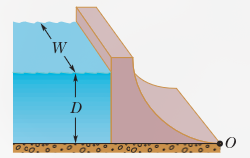
\includegraphics[width=0.45\linewidth]{images/24.png}
  \caption{Ilustrasi Grafik $p_2 - p_1$ terhadap $A_1^{-2}$ nomor 68}
  \label{fig:grafik-p-vs-A}
\end{figure}

\diketahui\ (dibaca dari grafik Gambar 14-52)
\begin{align*}
\Delta p_s &= \SI{3,00e5}{\pascal}, &
(p_2 - p_1)\big|_{A_1^{-2}=0} &= -\Delta p_s, &
(p_2 - p_1)\big|_{A_1^{-2}=32\,\si{\metre^{-4}}} &= +\Delta p_s
\end{align*}
Garis lurus memotong sumbu horizontal ($p_2 - p_1 = 0$) pada $A_1^{-2} = \SI{16}{\metre^{-4}}$.

\ditanya\ (a) $A_2$; (b) laju aliran volume $Q$.

\konsep\ Bernoulli (horizontal) dan kontinuitas dengan $v_1 = Q/A_1$, $v_2 = Q/A_2$ memberi
\begin{equation*}
p_2 - p_1 = \tfrac{1}{2}\rho\left(v_1^2 - v_2^2\right)
 = \tfrac{1}{2}\rho Q^2\left(A_1^{-2} - A_2^{-2}\right)
\end{equation*}
Ini adalah garis lurus terhadap $A_1^{-2}$ dengan gradien $\tfrac{1}{2}\rho Q^2$. Pada
$p_2 = p_1$ berlaku $A_1^{-2} = A_2^{-2}$.

\penyelesaian

\textbf{(a)} Titik potong dengan sumbu horizontal terjadi saat $A_1^{-2} = A_2^{-2} = \SI{16}{\metre^{-4}}$:
\begin{equation}
A_2 = \frac{1}{\sqrt{16}}\ \si{\metre\squared} = \SI{0,25}{\metre\squared}
\end{equation}

\textbf{(b)} Gradien garis: dari $(0,\,-\Delta p_s)$ ke $(32,\,+\Delta p_s)$,
\begin{align}
\frac{\Delta(p_2 - p_1)}{\Delta(A_1^{-2})} &= \frac{2(\SI{3,00e5}{\pascal})}{\SI{32}{\metre^{-4}}} = \SI{1,875e4}{\pascal\metre^{4}} = \tfrac{1}{2}\rho Q^2 \\
Q &= \sqrt{\frac{2(\SI{1,875e4}{\pascal\metre^{4}})}{\SI{1,00e3}{\kilo\gram\per\metre\cubed}}} = \SI{6,1}{\metre\cubed\per\second}
\end{align}

\begin{jawaban}
(a) $A_2 = \SI{0,25}{\metre\squared}$.\\
(b) $Q \approx \SI{6,1}{\metre\cubed\per\second}$.
\end{jawaban}

% =====================================================
\section*{Soal 69}
Cairan bermassa jenis $\SI{900}{\kilo\gram\per\metre\cubed}$ mengalir melalui pipa
horizontal yang memiliki luas penampang $\SI{1,90e-2}{\metre\squared}$ di daerah $A$ dan
$\SI{9,50e-3}{\metre\squared}$ di daerah $B$. Selisih tekanan antara kedua daerah adalah
$\SI{7,20e3}{\pascal}$. Berapa (a) laju aliran volume dan (b) laju aliran massa?

\diketahui
\begin{align*}
\rho &= \SI{900}{\kilo\gram\per\metre\cubed}, &
A_A &= \SI{1,90e-2}{\metre\squared}, &
A_B &= \SI{9,50e-3}{\metre\squared}, &
\Delta p &= p_A - p_B = \SI{7,20e3}{\pascal}
\end{align*}

\ditanya\ (a) $R_V$; (b) $R_m$.

\konsep\ Kontinuitas $A_A v_A = A_B v_B$ memberi $v_B = (A_A/A_B)\,v_A = 2v_A$. Bernoulli
(pipa horizontal): $p_A - p_B = \tfrac{1}{2}\rho\left(v_B^2 - v_A^2\right)$.

\penyelesaian

\textbf{(a)}
\begin{align}
\Delta p &= \tfrac{1}{2}\rho\left(4v_A^2 - v_A^2\right) = \tfrac{3}{2}\rho v_A^2 \\
v_A &= \sqrt{\frac{2\,\Delta p}{3\rho}} = \sqrt{\frac{2(\num{7,20e3})}{3(\num{900})}} = \SI{2,31}{\meter\per\second} \\
R_V &= A_A v_A = (\SI{1,90e-2}{\metre\squared})(\SI{2,31}{\meter\per\second}) = \SI{4,4e-2}{\metre\cubed\per\second}
\end{align}

\textbf{(b)}
\begin{equation}
R_m = \rho R_V = (\SI{900}{\kilo\gram\per\metre\cubed})(\SI{4,39e-2}{\metre\cubed\per\second}) = \SI{39}{\kilo\gram\per\second}
\end{equation}

\begin{jawaban}
(a) $R_V \approx \SI{4,4e-2}{\metre\cubed\per\second}$.\\
(b) $R_m \approx \SI{39}{\kilo\gram\per\second}$.
\end{jawaban}

% =====================================================
\section*{Soal 70}
Pada Gambar 14-53, air mengalir tunak dari bagian pipa kiri (jari-jari $r_1 = 2{,}00R$),
melalui bagian tengah (jari-jari $R$), dan ke bagian kanan (jari-jari $r_3 = 3{,}00R$).
Kelajuan air di bagian tengah $\SI{0,500}{\meter\per\second}$. Berapa usaha neto yang
dilakukan pada $\SI{0,400}{\metre\cubed}$ air ketika bergerak dari bagian kiri ke bagian kanan?

\begin{figure}[H]
  \centering
  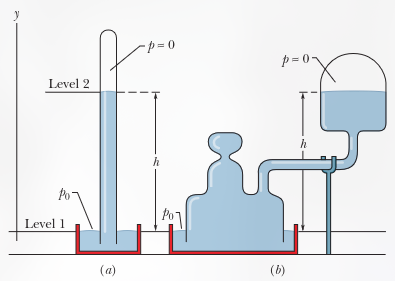
\includegraphics[width=0.45\linewidth]{images/25.png}
  \caption{Ilustrasi Pipa dengan Tiga Penampang nomor 70}
  \label{fig:pipa-tiga-bagian}
\end{figure}

\diketahui
\begin{align*}
r_1 &= 2{,}00R, &
r_2 &= R, &
r_3 &= 3{,}00R, &
v_2 &= \SI{0,500}{\meter\per\second}, &
V &= \SI{0,400}{\metre\cubed}
\end{align*}

\ditanya\ Usaha neto $W$ pada air.

\konsep\ Pipa horizontal sehingga energi potensial gravitasi tidak berubah. Menurut teorema
usaha--energi kinetik, usaha neto sama dengan perubahan energi kinetik:
$W = \Delta K = \tfrac{1}{2}\rho V\left(v_3^2 - v_1^2\right)$.
Kelajuan di tiap bagian diperoleh dari kontinuitas ($A \propto r^2$).

\penyelesaian
\begin{align}
v_1 &= v_2\left(\frac{R}{2R}\right)^2 = \frac{\SI{0,500}{\meter\per\second}}{4} = \SI{0,125}{\meter\per\second} \\
v_3 &= v_2\left(\frac{R}{3R}\right)^2 = \frac{\SI{0,500}{\meter\per\second}}{9} = \SI{0,0556}{\meter\per\second} \\
W &= \tfrac{1}{2}(\num{1,00e3})(\num{0,400})\left[(\num{0,0556})^2 - (\num{0,125})^2\right] \\
  &= (\SI{200}{\kilo\gram})(\num{3,09e-3} - \num{1,563e-2})\,\si{\metre\squared\per\second\squared} = -\SI{2,5}{\joule}
\end{align}

\begin{jawaban}
$W \approx -\SI{2,5}{\joule}$ (negatif karena air melambat dari bagian kiri ke kanan).
\end{jawaban}


% ---------------------------------------------------------------
\section*{Soal 71}
Gambar 14-54 menunjukkan aliran air melalui lubang pada kedalaman $h = \SI{10}{\centi\meter}$
dalam tangki berisi air setinggi $H = \SI{40}{\centi\meter}$.
(a) Pada jarak $x$ berapa aliran air menyentuh lantai?
(b) Pada kedalaman berapa lubang kedua harus dibuat agar menghasilkan nilai $x$ yang sama?
(c) Pada kedalaman berapa lubang harus dibuat agar $x$ maksimum?
 
\begin{figure}[H]
  \centering
  \IfFileExists{images/26.png}
    {\includegraphics[width=0.35\linewidth]{images/26.png}}
    {\fbox{\parbox{0.35\linewidth}{\centering Gambar 14-54}}}
  \caption{Ilustrasi aliran air dari lubang tangki nomor 71}
  \label{fig:tangki-lubang}
\end{figure}
 
\diketahui
\begin{align*}
h &= \SI{10}{\centi\meter} = \SI{0,10}{\meter}, &
H &= \SI{40}{\centi\meter} = \SI{0,40}{\meter}
\end{align*}
 
\ditanya\ (a) $x$; (b) kedalaman lubang kedua $h'$ untuk $x$ yang sama; (c) $h$ untuk $x$ maksimum.
 
\konsep\ Kelajuan semburan di lubang mengikuti teorema Torricelli, $v = \sqrt{2gh}$
(Bernoulli antara permukaan air dan lubang). Setelah keluar, air bergerak sebagai gerak
parabola dengan kecepatan awal horizontal $v$ dari ketinggian $H-h$ di atas lantai, sehingga
waktu jatuh $t = \sqrt{2(H-h)/g}$ dan jarak horizontal $x = vt$.
 
\penyelesaian
 
\textbf{(a)} Jarak jangkauan secara umum:
\begin{align*}
x = vt = \sqrt{2gh}\,\sqrt{\frac{2(H-h)}{g}} = 2\sqrt{h\,(H-h)}
\end{align*}
Dengan data soal:
\begin{align*}
x = 2\sqrt{(\num{0,10})(\num{0,40}-\num{0,10})}\ \si{\meter}
  = 2\sqrt{\num{0,030}}\ \si{\meter} = \SI{0,35}{\meter}
\end{align*}
 
\textbf{(b)} Nilai $x$ sama bila $h'(H-h') = h(H-h)$. Persamaan kuadrat
$h'^2 - Hh' + h(H-h) = 0$ memiliki dua akar, yaitu $h' = h$ dan $h' = H - h$. Jadi
\begin{align*}
h' = H - h = \SI{40}{\centi\meter} - \SI{10}{\centi\meter} = \SI{30}{\centi\meter}
\end{align*}
 
\textbf{(c)} $x$ maksimum bila $h(H-h)$ maksimum:
\begin{align*}
\frac{d}{dh}\left[h(H-h)\right] = H - 2h = 0 \quad\Rightarrow\quad h = \frac{H}{2} = \SI{20}{\centi\meter}
\end{align*}
Pada kedalaman ini $x_{\text{maks}} = 2\sqrt{(H/2)^2} = H = \SI{0,40}{\meter}$.
 
\begin{jawaban}
(a) $x \approx \SI{0,35}{\meter}$ \quad (b) $h' = \SI{30}{\centi\meter}$ (simetris terhadap $h$ terhadap titik $H/2$)
\quad (c) $h = \SI{20}{\centi\meter}$, dengan $x_{\text{maks}} = \SI{0,40}{\meter}$.
\end{jawaban}
 
% ---------------------------------------------------------------
\section*{Soal 72}
Gambar 14-55 menunjukkan sistem drainase air hujan yang disederhanakan untuk sebuah rumah.
Air hujan dari atap mengalir ke talang, lalu melalui pipa tegak (\textit{downspout}) menuju
pipa drainase utama $M$ di bawah ruang bawah tanah. Saluran lantai di ruang bawah tanah juga
terhubung ke pipa $M$. Anggap: (1) tinggi pipa tegak $h_1 = \SI{11}{\meter}$;
(2) tinggi saluran lantai $h_2 = \SI{1,2}{\meter}$; (3) jari-jari pipa $M$ adalah $\SI{3,0}{\centi\meter}$;
(4) lebar sisi rumah $w = \SI{30}{\meter}$ dan panjang muka $L = \SI{60}{\meter}$;
(5) seluruh air hujan yang mengenai atap masuk ke pipa $M$; (6) kelajuan awal air di pipa tegak
dapat diabaikan; (7) kelajuan angin dapat diabaikan (hujan jatuh vertikal).
Pada laju curah hujan berapa (dalam cm/jam) air dari pipa $M$ mencapai ketinggian saluran lantai
dan mengancam membanjiri ruang bawah tanah?
 
\begin{figure}[H]
  \centering
  \IfFileExists{images/27.png}
    {\includegraphics[width=0.4\linewidth]{images/27.png}}
    {\fbox{\parbox{0.4\linewidth}{\centering Gambar 14-55}}}
  \caption{Skema sistem drainase air hujan nomor 72}
  \label{fig:drainase}
\end{figure}
 
\diketahui
\begin{align*}
h_1 &= \SI{11}{\meter}, & h_2 &= \SI{1,2}{\meter}, & r_M &= \SI{3,0}{\centi\meter} = \SI{0,030}{\meter}, \\
w &= \SI{30}{\meter}, & L &= \SI{60}{\meter}, & \rho &= \SI{1,00e3}{\kilo\gram\per\metre\cubed}
\end{align*}
 
\ditanya\ Laju curah hujan $R$ (cm/jam) saat air di pipa $M$ mencapai ketinggian saluran lantai.
 
\konsep\ Air mulai meluap ke saluran lantai ketika tekanan di pipa $M$ pada ketinggian $h_2$
sama dengan tekanan atmosfer $p_0$. Persamaan Bernoulli diterapkan antara puncak pipa tegak
(tekanan $p_0$, kelajuan $\approx 0$, ketinggian $h_1$ di atas pipa $M$) dan titik di pipa $M$
pada ketinggian $h_2$ (tekanan $p_0$, kelajuan $v$). Kekekalan debit menghubungkan $v$ dengan
laju curah hujan: $R\,(wL) = A_M v$.
 
\penyelesaian
 
Bernoulli:
\begin{align*}
p_0 + \rho g h_1 + 0 &= p_0 + \rho g h_2 + \tfrac{1}{2}\rho v^2 \\
v &= \sqrt{2g(h_1 - h_2)} = \sqrt{2(\num{9,8})(\num{11}-\num{1,2})}\ \si{\meter\per\second} = \SI{13,9}{\meter\per\second}
\end{align*}
Debit air di pipa $M$:
\begin{align*}
Q = A_M v = \pi r_M^2 v = \pi(\num{0,030})^2(\num{13,86})\ \si{\metre\cubed\per\second} = \SI{3,92e-2}{\metre\cubed\per\second}
\end{align*}
Laju curah hujan (volume air per satuan waktu per luas atap $wL$):
\begin{align*}
R = \frac{Q}{wL} = \frac{\num{3,92e-2}}{(30)(60)}\ \si{\meter\per\second}
  = \SI{2,18e-5}{\meter\per\second}
  = \SI{2,18e-5}{} \times \num{3,6e5}\ \si{\centi\meter\per\hour} \approx \SI{7,8}{\centi\meter\per\hour}
\end{align*}
 
\begin{jawaban}
$R \approx \SI{7,8}{\centi\meter\per\hour}$
\end{jawaban}
 
% ---------------------------------------------------------------
\section*{Soal 73}
Sekitar sepertiga bagian tubuh seseorang yang mengapung di Laut Mati berada di atas permukaan air.
Dengan menganggap massa jenis tubuh manusia $\SI{0,98}{\gram\per\centi\meter\cubed}$, tentukan massa jenis air
Laut Mati. (Mengapa nilainya jauh lebih besar daripada $\SI{1,0}{\gram\per\centi\meter\cubed}$?)
 
\diketahui
\begin{align*}
\rho_{\text{tubuh}} = \SI{0,98}{\gram\per\centi\meter\cubed} = \SI{980}{\kilo\gram\per\metre\cubed}, \qquad
\frac{V_{\text{tercelup}}}{V} = 1 - \frac{1}{3} = \frac{2}{3}
\end{align*}
 
\ditanya\ Massa jenis air Laut Mati $\rho_{\text{LM}}$.
 
\konsep\ Pada benda yang mengapung, gaya apung sama dengan berat benda (Hukum Archimedes):
$\rho_{\text{LM}}\,V_{\text{tercelup}}\,g = \rho_{\text{tubuh}}\,V g$.
 
\penyelesaian
\begin{align*}
\rho_{\text{LM}} = \rho_{\text{tubuh}}\,\frac{V}{V_{\text{tercelup}}}
= (\SI{0,98}{\gram\per\centi\meter\cubed})\left(\frac{3}{2}\right) = \SI{1,5}{\gram\per\centi\meter\cubed}
\end{align*}
 
Massa jenis air Laut Mati jauh lebih besar daripada air tawar karena kadar garam terlarutnya
sangat tinggi (salinitas sekitar $\SI{30}{\percent}$, kira-kira sembilan kali salinitas laut biasa).
Hal ini terjadi akibat penguapan yang sangat besar pada cekungan tertutup tanpa saluran keluar,
sehingga garam-garam mineral terus terakumulasi.
 
\begin{jawaban}
$\rho_{\text{LM}} \approx \SI{1,5}{\gram\per\centi\meter\cubed} = \SI{1,5e3}{\kilo\gram\per\metre\cubed}$
\end{jawaban}
 
% ---------------------------------------------------------------
\section*{Soal 74}
Sebuah pipa U terbuka sederhana berisi raksa. Ketika air setinggi $\SI{11,2}{\centi\meter}$ dituangkan
ke lengan kanan pipa, berapa tinggi kenaikan raksa di lengan kiri dari ketinggian awalnya?
 
\diketahui
\begin{align*}
h_{\text{air}} = \SI{11,2}{\centi\meter}, \quad
\rho_{\text{air}} = \SI{1,00e3}{\kilo\gram\per\metre\cubed}, \quad
\rho_{\text{Hg}} = \SI{13,6e3}{\kilo\gram\per\metre\cubed}
\end{align*}
 
\ditanya\ Kenaikan permukaan raksa di lengan kiri, $x$.
 
\konsep\ Penampang kedua lengan sama, sehingga bila raksa di lengan kanan turun sejauh $x$,
raksa di lengan kiri naik sejauh $x$ dan selisih tinggi permukaan raksa adalah $2x$.
Tekanan pada titik-titik di fluida yang sama pada ketinggian yang sama haruslah sama. Ambil
bidang acuan di permukaan raksa lengan kanan (batas air--raksa): tekanan di sisi kanan berasal
dari kolom air, sedangkan di sisi kiri berasal dari kolom raksa setinggi $2x$ (tekanan atmosfer
$p_0$ bekerja di kedua ujung terbuka dan saling meniadakan).
 
\penyelesaian
\begin{align*}
p_0 + \rho_{\text{air}}\, g\, h_{\text{air}} &= p_0 + \rho_{\text{Hg}}\, g\,(2x) \\
x &= \frac{\rho_{\text{air}}}{\rho_{\text{Hg}}}\,\frac{h_{\text{air}}}{2}
   = \frac{\num{1,00e3}}{\num{13,6e3}}\cdot\frac{\SI{11,2}{\centi\meter}}{2}
   = \SI{0,412}{\centi\meter}
\end{align*}
 
\begin{jawaban}
$x \approx \SI{0,412}{\centi\meter}$ (raksa di lengan kiri naik $\approx \SI{4,1}{\milli\meter}$).
\end{jawaban}
 
% ---------------------------------------------------------------
\section*{Soal 75}
Jika sebuah gelembung dalam air berkarbonasi (\textit{sparkling water}) dipercepat ke atas
dengan percepatan $\SI{0,225}{\meter\per\second\squared}$ dan berjari-jari $\SI{0,500}{\milli\meter}$,
berapakah massanya? Anggap gaya hambat pada gelembung dapat diabaikan.
 
\diketahui
\begin{align*}
a &= \SI{0,225}{\meter\per\second\squared}, &
r &= \SI{0,500}{\milli\meter} = \SI{5,00e-4}{\meter}, &
\rho_{\text{air}} &= \SI{1,00e3}{\kilo\gram\per\metre\cubed}
\end{align*}
 
\ditanya\ Massa gelembung $m$.
 
\konsep\ Gaya yang bekerja pada gelembung hanyalah gaya apung $F_b = \rho_{\text{air}} V g$ ke atas
(volume air yang dipindahkan sama dengan volume gelembung) dan berat $mg$ ke bawah. Hukum II Newton:
$F_b - mg = ma$.
 
\penyelesaian
 
Volume gelembung:
\begin{align*}
V = \frac{4}{3}\pi r^3 = \frac{4}{3}\pi(\num{5,00e-4})^3\ \si{\metre\cubed} = \SI{5,24e-10}{\metre\cubed}
\end{align*}
Dari Hukum II Newton:
\begin{align*}
\rho_{\text{air}} V g - mg &= ma \\
m &= \frac{\rho_{\text{air}} V g}{g + a}
   = \frac{(\num{1,00e3})(\num{5,24e-10})(\num{9,8})}{\num{9,8}+\num{0,225}}\ \si{\kilo\gram}
   = \SI{5,12e-7}{\kilo\gram}
\end{align*}
 
\begin{jawaban}
$m \approx \SI{5,12e-7}{\kilo\gram} = \SI{0,512}{\milli\gram}$
\end{jawaban}

% ---------------------------------------------------------------
\section*{Soal 76}
Misalkan tubuhmu memiliki massa jenis seragam sebesar $0{,}95$ kali massa jenis air.
(a) Jika kamu mengapung di kolam renang, berapa fraksi volume tubuhmu yang berada di atas permukaan air?
\textit{Quicksand} (pasir apung) adalah fluida yang terbentuk ketika air terdorong naik ke dalam pasir,
menggeser butir-butir pasir sehingga tidak lagi terkunci oleh gesekan. Kolam \textit{quicksand} dapat
terbentuk ketika air mengalir di bawah tanah dari perbukitan ke lembah yang memiliki kantong pasir.
(b) Jika kamu mengapung di kolam \textit{quicksand} yang dalam dengan massa jenis $1{,}6$ kali massa jenis air,
berapa fraksi volume tubuhmu yang berada di atas permukaan \textit{quicksand}?
(c) Apakah kamu tidak dapat bernapas?
 
\diketahui
\begin{align*}
\rho_{\text{tubuh}} = 0{,}95\,\rho_{\text{air}}, \qquad
\rho_{\text{qs}} = 1{,}6\,\rho_{\text{air}}
\end{align*}
 
\ditanya\ (a) Fraksi volume di atas permukaan air; (b) fraksi volume di atas permukaan \textit{quicksand};
(c) apakah pernapasan terganggu.
 
\konsep\ Benda yang mengapung berada dalam kesetimbangan: gaya apung sama dengan berat benda,
$\rho_f V_{\text{tc}}\, g = \rho_{\text{tubuh}} V g$, sehingga fraksi volume yang tercelup adalah
\begin{align*}
\frac{V_{\text{tc}}}{V} = \frac{\rho_{\text{tubuh}}}{\rho_f}
\end{align*}
dan fraksi volume yang berada di atas permukaan adalah $1 - V_{\text{tc}}/V$.
 
\penyelesaian
 
\textbf{(a)} Untuk air:
\begin{align*}
\frac{V_{\text{tc}}}{V} = \frac{0{,}95\,\rho_{\text{air}}}{\rho_{\text{air}}} = 0{,}95
\quad\Rightarrow\quad
\text{fraksi di atas permukaan} = 1 - 0{,}95 = 0{,}05
\end{align*}
 
\textbf{(b)} Untuk \textit{quicksand}:
\begin{align*}
\frac{V_{\text{tc}}}{V} = \frac{0{,}95}{1{,}6} = 0{,}594
\quad\Rightarrow\quad
\text{fraksi di atas permukaan} = 1 - 0{,}594 = 0{,}41
\end{align*}
 
\textbf{(c)} Tidak. Dalam model ini sekitar $\SI{41}{\percent}$ volume tubuh berada di atas permukaan
\textit{quicksand}, sehingga kepala dan dada dapat berada di atas permukaan dan pernapasan tidak terhalang.
Bahkan, seseorang akan mengapung lebih tinggi dibandingkan di kolam renang.
 
\begin{jawaban}
(a) $\SI{5}{\percent}$ \quad (b) $\approx \SI{41}{\percent}$ \quad (c) Tidak; kita dapat bernapas karena kepala berada di atas permukaan.
\end{jawaban}
 
% ---------------------------------------------------------------
\section*{Soal 77}
Sebuah bola kaca berjari-jari $\SI{2,00}{\centi\meter}$ berada di dasar wadah berisi susu dengan massa jenis
$\SI{1,03}{\gram\per\centi\meter\cubed}$. Gaya normal dari permukaan bawah wadah pada bola memiliki besar
$\SI{9,48e-2}{\newton}$. Berapakah massa bola tersebut?
 
\diketahui
\begin{align*}
r &= \SI{2,00}{\centi\meter} = \SI{2,00e-2}{\meter}, &
\rho_{\text{susu}} &= \SI{1,03}{\gram\per\centi\meter\cubed} = \SI{1,03e3}{\kilo\gram\per\metre\cubed}, &
N &= \SI{9,48e-2}{\newton}
\end{align*}
 
\ditanya\ Massa bola $m$.
 
\konsep\ Bola diam di dasar wadah, sehingga resultan gaya vertikalnya nol. Gaya ke atas terdiri atas
gaya normal $N$ dan gaya apung $F_b = \rho_{\text{susu}} V g$, sedangkan gaya ke bawah adalah berat $mg$:
\begin{align*}
N + F_b = mg
\end{align*}
 
\penyelesaian
 
Volume bola:
\begin{align*}
V = \frac{4}{3}\pi r^3 = \frac{4}{3}\pi(\num{2,00e-2})^3\ \si{\metre\cubed} = \SI{3,35e-5}{\metre\cubed}
\end{align*}
Massa bola:
\begin{align*}
m &= \frac{N}{g} + \rho_{\text{susu}} V
   = \frac{\num{9,48e-2}}{\num{9,8}} + (\num{1,03e3})(\num{3,351e-5})\ \si{\kilo\gram} \\
  &= \num{9,67e-3} + \num{3,45e-2}\ \si{\kilo\gram} = \SI{4,42e-2}{\kilo\gram}
\end{align*}
 
\begin{jawaban}
$m \approx \SI{4,42e-2}{\kilo\gram} = \SI{44,2}{\gram}$
\end{jawaban}
 
% ---------------------------------------------------------------
\section*{Soal 78}
Seorang pemain ski terjebak dalam longsoran salju dan tenggelam sepenuhnya dalam salju yang mengalir
dengan massa jenis $\SI{96}{\kilo\gram\per\metre\cubed}$. Anggap massa jenis rata-rata pemain ski, pakaian,
dan peralatan ski adalah $\SI{1020}{\kilo\gram\per\metre\cubed}$. Berapa persen gaya gravitasi pada pemain ski
yang diimbangi oleh gaya apung dari salju?
 
\diketahui
\begin{align*}
\rho_{\text{salju}} = \SI{96}{\kilo\gram\per\metre\cubed}, \qquad
\rho_{\text{ski}} = \SI{1020}{\kilo\gram\per\metre\cubed}
\end{align*}
 
\ditanya\ Persentase $F_b/(mg)$.
 
\konsep\ Karena tenggelam sepenuhnya, volume salju yang dipindahkan sama dengan volume pemain ski $V$.
Gaya apung $F_b = \rho_{\text{salju}} V g$ dan berat $mg = \rho_{\text{ski}} V g$.
 
\penyelesaian
\begin{align*}
\frac{F_b}{mg} = \frac{\rho_{\text{salju}}\, V g}{\rho_{\text{ski}}\, V g}
= \frac{\rho_{\text{salju}}}{\rho_{\text{ski}}}
= \frac{96}{1020} = 0{,}094 = \SI{9,4}{\percent}
\end{align*}
 
\begin{jawaban}
Gaya apung mengimbangi $\approx \SI{9,4}{\percent}$ gaya gravitasi pada pemain ski.
\end{jawaban}
 
% ---------------------------------------------------------------
\section*{Soal 79}
Sebuah benda digantung pada neraca pegas. Neraca menunjukkan $\SI{30}{\newton}$ di udara,
$\SI{20}{\newton}$ ketika benda dicelupkan ke dalam air, dan $\SI{24}{\newton}$ ketika benda dicelupkan ke dalam
cairan lain yang massa jenisnya tidak diketahui. Berapakah massa jenis cairan lain tersebut?
 
\diketahui
\begin{align*}
W_{\text{udara}} = \SI{30}{\newton}, \quad
W_{\text{air}} = \SI{20}{\newton}, \quad
W_{\text{cairan}} = \SI{24}{\newton}, \quad
\rho_{\text{air}} = \SI{1,00e3}{\kilo\gram\per\metre\cubed}
\end{align*}
 
\ditanya\ Massa jenis cairan $\rho_x$.
 
\konsep\ Bacaan neraca pegas pada benda yang tercelup adalah berat semu, $W_{\text{app}} = W - F_b$.
Dengan benda yang sama tercelup penuh, volume fluida yang dipindahkan sama, sehingga gaya apung
sebanding dengan massa jenis fluida: $F_b = \rho_f V g$.
 
\penyelesaian
 
Gaya apung pada tiap fluida:
\begin{align*}
F_{b,\text{air}} &= 30 - 20 = \SI{10}{\newton}, &
F_{b,x} &= 30 - 24 = \SI{6}{\newton}
\end{align*}
Perbandingan kedua gaya apung memberikan
\begin{align*}
\frac{\rho_x}{\rho_{\text{air}}} = \frac{F_{b,x}}{F_{b,\text{air}}} = \frac{6}{10} = 0{,}60
\quad\Rightarrow\quad
\rho_x = 0{,}60\,(\SI{1,00e3}{\kilo\gram\per\metre\cubed}) = \SI{6,0e2}{\kilo\gram\per\metre\cubed}
\end{align*}
 
\begin{jawaban}
$\rho_x = \SI{6,0e2}{\kilo\gram\per\metre\cubed} = \SI{0,60}{\gram\per\centi\meter\cubed}$
\end{jawaban}
 
% ---------------------------------------------------------------
\section*{Soal 80}
Dalam sebuah percobaan, sebuah balok persegi panjang setinggi $h$ dibiarkan mengapung dalam empat cairan
berbeda. Pada cairan pertama, yaitu air, balok mengapung dengan tercelup sepenuhnya. Pada cairan $A$, $B$,
dan $C$, balok mengapung dengan tinggi $h/2$, $2h/3$, dan $h/4$ di atas permukaan cairan.
Berapakah massa jenis relatif (massa jenis terhadap air) dari (a) $A$, (b) $B$, dan (c) $C$?
 
\diketahui
\begin{align*}
h_{\text{atas},A} = \frac{h}{2}, \qquad
h_{\text{atas},B} = \frac{2h}{3}, \qquad
h_{\text{atas},C} = \frac{h}{4}
\end{align*}
Pada air, balok tercelup seluruhnya ($V_{\text{tc}} = V$).
 
\ditanya\ Massa jenis relatif $\rho_A/\rho_{\text{air}}$, $\rho_B/\rho_{\text{air}}$, dan $\rho_C/\rho_{\text{air}}$.
 
\konsep\ Karena balok mengapung tepat tercelup seluruhnya di air, massa jenis balok sama dengan massa jenis air:
$\rho_{\text{balok}} = \rho_{\text{air}}$. Untuk cairan mana pun, kesetimbangan apung memberikan
$\rho_f V_{\text{tc}} = \rho_{\text{balok}} V$. Karena penampang balok seragam, fraksi volume
tercelup sama dengan fraksi tinggi tercelup:
\begin{align*}
\frac{\rho_f}{\rho_{\text{air}}} = \frac{V}{V_{\text{tc}}} = \frac{h}{h_{\text{tc}}}
\end{align*}
 
\penyelesaian
 
\textbf{(a)} Cairan $A$: $h_{\text{tc}} = h - \dfrac{h}{2} = \dfrac{h}{2}$
\begin{align*}
\frac{\rho_A}{\rho_{\text{air}}} = \frac{h}{h/2} = 2{,}00
\end{align*}
 
\textbf{(b)} Cairan $B$: $h_{\text{tc}} = h - \dfrac{2h}{3} = \dfrac{h}{3}$
\begin{align*}
\frac{\rho_B}{\rho_{\text{air}}} = \frac{h}{h/3} = 3{,}00
\end{align*}
 
\textbf{(c)} Cairan $C$: $h_{\text{tc}} = h - \dfrac{h}{4} = \dfrac{3h}{4}$
\begin{align*}
\frac{\rho_C}{\rho_{\text{air}}} = \frac{h}{3h/4} = \frac{4}{3} = 1{,}33
\end{align*}
 
\begin{jawaban}
(a) $\rho_A/\rho_{\text{air}} = 2{,}00$ \quad (b) $\rho_B/\rho_{\text{air}} = 3{,}00$ \quad (c) $\rho_C/\rho_{\text{air}} \approx 1{,}33$
\end{jawaban}

\section*{Soal 81}
Gambar 14-30 menunjukkan tabung berbentuk U yang dimodifikasi. Lengan kanan lebih pendek daripada lengan kiri. Ujung terbuka lengan kanan berada pada ketinggian $d=\SI{10,0}{\centi\metre}$ di atas meja. Jari-jari tabung adalah $r=\SI{1,50}{\centi\metre}$. Air dituangkan ke lengan kiri sampai mulai mengalir keluar dari lengan kanan. Kemudian cairan dengan massa jenis $0,80\ \si{\gram\per\centi\metre\cubed}$ dituangkan ke lengan kiri hingga tinggi kolom cairan tersebut \SI{8,0}{\centi\metre}. Tentukan volume air yang mengalir keluar dari lengan kanan.

\diketahui
\begin{align*}
d &= \SI{10,0}{\centi\metre}, &
r &= \SI{1,50}{\centi\metre},\\
\rho_\ell &= 0,80\,\rho_w, &
h_\ell &= \SI{8,0}{\centi\metre}.
\end{align*}
\ditanya\ Volume air yang keluar, $V_{\mathrm{keluar}}$.

\konsep\ Pada keadaan setimbang, tekanan pada ketinggian yang sama dalam fluida yang saling terhubung adalah sama. Karena lengan kanan terbuka dan air berada tepat di bibir lengan, penurunan antarmuka air--cairan di lengan kiri sebesar $x$ memenuhi
\[
\rho_w g x=\rho_\ell g h_\ell.
\]
Volume air yang keluar sama dengan luas penampang tabung dikalikan penurunan tinggi kolom air tersebut.

\penyelesaian
\begin{align*}
x &= \frac{\rho_\ell}{\rho_w}h_\ell
   = (0,80)(\SI{8,0}{\centi\metre})\\
  &= \SI{6,4}{\centi\metre},\\[4pt]
A &= \pi r^2
   = \pi(\SI{1,50}{\centi\metre})^2\\
  &= \SI{7,07}{\centi\metre\squared},\\[4pt]
V_{\mathrm{keluar}} &= Ax\\
  &= (\SI{7,07}{\centi\metre\squared})
     (\SI{6,4}{\centi\metre})\\
  &= \SI{45}{\centi\metre\cubed}.
\end{align*}
\begin{jawaban}
Volume air yang mengalir keluar adalah
\[
\boxed{V_{\mathrm{keluar}}\approx\SI{45}{\centi\metre\cubed}
=\SI{4,5e-5}{\metre\cubed}.}
\]
\end{jawaban}

\section*{Soal 82}
Sebuah balon udara panas naik ketika massa jenis udara di luar balon lebih besar daripada massa jenis udara di dalamnya. Jika perbandingan massa jenis udara luar terhadap udara dalam adalah $1,39$, tentukan percepatan balon. Massa balon dan keranjangnya diabaikan.

\diketahui
\[
\frac{\rho_{\mathrm{luar}}}{\rho_{\mathrm{dalam}}}=1,39.
\]
\ditanya\ Percepatan balon, $a$.

\konsep\ Gaya apung adalah $F_A=\rho_{\mathrm{luar}}Vg$, sedangkan berat udara di dalam balon adalah $w=\rho_{\mathrm{dalam}}Vg$. Dengan mengabaikan massa kain balon dan keranjang, massa sistem yang dipercepat adalah massa udara di dalam balon, $m=\rho_{\mathrm{dalam}}V$. Hukum II Newton memberikan
\[
a=\frac{F_A-w}{m}
=\left(\frac{\rho_{\mathrm{luar}}}{\rho_{\mathrm{dalam}}}-1\right)g.
\]

\penyelesaian
\begin{align*}
a &= (1,39-1)(\SI{9,8}{\metre\per\second\squared})\\
  &= \SI{3,82}{\metre\per\second\squared}.
\end{align*}
\begin{jawaban}
\[
\boxed{a=\SI{3,8}{\metre\per\second\squared}\text{ ke atas}.}
\]
\end{jawaban}

\section*{Soal 83}
Sebuah sifon digunakan untuk mengalirkan cairan bermassa jenis $\rho=\SI{1000}{\kilogram\per\metre\cubed}$. Diketahui $h_1=\SI{25}{\centi\metre}$, $d=\SI{12}{\centi\metre}$, dan $h_2=\SI{40}{\centi\metre}$. Anggap viskositas dapat diabaikan. Tentukan (a) kelajuan cairan saat keluar di titik C, (b) tekanan di titik tertinggi B jika tekanan atmosfer \SI{1,0e5}{\pascal}, dan (c) nilai maksimum teoretis $h_1$.

\begin{figure}[H]
  \centering
  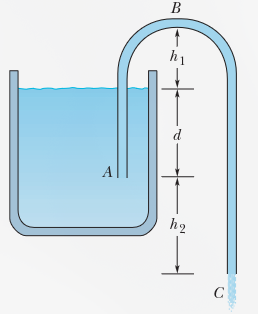
\includegraphics[width=0.45\linewidth]{images/83.png}
  \caption{Ilustrasi sifon nomor 83}
  \label{fig:sifon}
\end{figure}

\diketahui
\begin{align*}
\rho &= \SI{1000}{\kilogram\per\metre\cubed},&
h_1 &= \SI{0,25}{\metre},\\
d &= \SI{0,12}{\metre},&
h_2 &= \SI{0,40}{\metre},\\
p_{\mathrm{atm}} &= \SI{1,0e5}{\pascal}.
\end{align*}
\ditanya\ (a) Kelajuan di C, $v_C$; (b) tekanan di B, $p_B$; (c) $h_{1,\max}$.

\konsep\ Gunakan persamaan Bernoulli antara permukaan bebas cairan dan titik keluaran C. Kecepatan permukaan bebas dianggap nol dan tekanan di permukaan serta di keluaran sama-sama tekanan atmosfer. Untuk titik B, persamaan Bernoulli diterapkan antara permukaan bebas dan titik tertinggi. Nilai maksimum teoretis $h_1$ diperoleh dengan batas tekanan absolut di B sama dengan nol.

\penyelesaian

\noindent\textbf{(a) Kelajuan cairan di C}
\begin{align*}
p_{\mathrm{atm} }+\rho g h_2
&=p_{\mathrm{atm}}+\frac12\rho v_C^2,\\
v_C&=\sqrt{2gh_2}\\
&=\sqrt{2(\SI{9,8}{\metre\per\second\squared})(\SI{0,40}{\metre})}\\
&=\SI{2,8}{\metre\per\second}.
\end{align*}

\noindent\textbf{(b) Tekanan di titik B}
\begin{align*}
p_{\mathrm{atm}}
&=p_B+\rho g h_1+\frac12\rho v_C^2,\\
p_B&=p_{\mathrm{atm}}-\rho g(h_1+h_2)\\
&=\SI{1,0e5}{\pascal}
-(\SI{1000}{\kilogram\per\metre\cubed})
(\SI{9,8}{\metre\per\second\squared})(\SI{0,65}{\metre})\\
&=\SI{9,36e4}{\pascal}.
\end{align*}

\noindent\textbf{(c) Ketinggian maksimum teoretis}
Pada batas teoretis $p_B=0$:
\begin{align*}
0&=p_{\mathrm{atm}}-\rho g(h_{1,\max}+h_2),\\
h_{1,\max}&=\frac{p_{\mathrm{atm}}}{\rho g}-h_2\\
&=\frac{\SI{1,0e5}{\pascal}}
{(\SI{1000}{\kilogram\per\metre\cubed})(\SI{9,8}{\metre\per\second\squared})}
-\SI{0,40}{\metre}\\
&=\SI{9,8}{\metre}.
\end{align*}
\begin{jawaban}
\[
\boxed{v_C=\SI{2,8}{\metre\per\second}},\qquad
\boxed{p_B\approx\SI{9,36e4}{\pascal}},\qquad
\boxed{h_{1,\max}\approx\SI{9,8}{\metre}}.
\]
Nilai maksimum pada (c) merupakan batas ideal ketika tekanan absolut di puncak sifon nol; pada keadaan nyata, tekanan uap cairan membatasi ketinggian lebih lanjut.
\end{jawaban}

\section*{Soal 84}
Saat batuk, udara dikeluarkan melalui trakea dengan laju aliran volume $Q=\SI{7,0e-3}{\metre\cubed\per\second}$. Tentukan kelajuan udara sebagai kelipatan kelajuan bunyi $v_s=\SI{343}{\metre\per\second}$ jika diameter trakea (a) tetap \SI{14}{\milli\metre} dan (b) menyempit menjadi \SI{5,2}{\milli\metre}.

\diketahui
\[
Q=\SI{7,0e-3}{\metre\cubed\per\second},\qquad
v_s=\SI{343}{\metre\per\second}.
\]
\ditanya\ Rasio $v/v_s$ untuk kedua diameter.

\konsep\ Persamaan kontinuitas untuk laju aliran volume adalah $Q=Av$. Untuk penampang lingkaran, $A=\pi d^2/4$, sehingga
\[
v=\frac{4Q}{\pi d^2}.
\]

\penyelesaian

\noindent\textbf{(a) Diameter trakea \SI{14}{\milli\metre}}
\begin{align*}
d_1&=\SI{0,014}{\metre},\\
v_1&=\frac{4(\SI{7,0e-3}{\metre\cubed\per\second})}
{\pi(\SI{0,014}{\metre})^2}\\
&=\SI{45,5}{\metre\per\second},\\
\frac{v_1}{v_s}&=\frac{45,5}{343}=0,133.
\end{align*}

\noindent\textbf{(b) Diameter trakea \SI{5,2}{\milli\metre}}
\begin{align*}
d_2&=\SI{0,0052}{\metre},\\
v_2&=\frac{4(\SI{7,0e-3}{\metre\cubed\per\second})}
{\pi(\SI{0,0052}{\metre})^2}\\
&=\SI{330}{\metre\per\second},\\
\frac{v_2}{v_s}&=\frac{330}{343}=0,96.
\end{align*}
\begin{jawaban}
\[
\boxed{v_1\approx0,13v_s},\qquad
\boxed{v_2\approx0,96v_s}.
\]
\end{jawaban}

\section*{Soal 85}
Sebuah kaleng memiliki volume total \SI{1200}{\centi\metre\cubed} dan massa \SI{130}{\gram}. Berapa massa maksimum gotri timbal bermassa jenis \SI{11,4}{\gram\per\centi\metre\cubed} yang dapat dibawa kaleng tanpa tenggelam di air?

\begin{figure}[H]
  \centering
  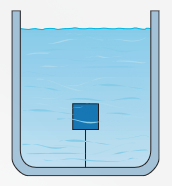
\includegraphics[width=0.45\linewidth]{images/85.png}
  \caption{Ilustrasi Kaleng nomor 85}
  \label{fig:can}
\end{figure}

\diketahui
\begin{align*}
V_{\mathrm{kaleng}}&=\SI{1200}{\centi\metre\cubed},\\
m_{\mathrm{kaleng}}&=\SI{130}{\gram},\\
\rho_{\mathrm{Pb}}&=\SI{11,4}{\gram\per\centi\metre\cubed},\\
\rho_w&=\SI{1,00}{\gram\per\centi\metre\cubed}.
\end{align*}
\ditanya\ Massa maksimum gotri timbal, $m_{\mathrm{Pb}}$.

\konsep\ Pada keadaan tepat sebelum tenggelam, gaya apung maksimum sama dengan berat total kaleng dan muatannya. Kaleng dapat memindahkan air dengan massa maksimum $\rho_wV_{\mathrm{kaleng}}$. Karena gotri berada di dalam kaleng, volume luar yang memindahkan air tetap sebesar volume kaleng.

\penyelesaian
\begin{align*}
m_{\mathrm{total,max}}&=\rho_wV_{\mathrm{kaleng}}\\
&=(\SI{1,00}{\gram\per\centi\metre\cubed})
(\SI{1200}{\centi\metre\cubed})\\
&=\SI{1200}{\gram},\\[4pt]
m_{\mathrm{Pb,max}}&=m_{\mathrm{total,max}}-m_{\mathrm{kaleng}}\\
&=\SI{1200}{\gram}-\SI{130}{\gram}\\
&=\SI{1070}{\gram}.
\end{align*}
\begin{jawaban}
Massa maksimum gotri timbal yang dapat dibawa adalah
\[
\boxed{m_{\mathrm{Pb,max}}=\SI{1,07e3}{\gram}\approx\SI{1,07}{\kilogram}.}
\]
\end{jawaban}

\section*{Nomor 86}
Sebuah balok padat ditahan oleh tali di bawah permukaan cairan yang massa jenisnya lebih besar daripada massa jenis balok. Saat wadah diam, tegangan tali adalah $T_0$. Tentukan tegangan tali ketika wadah dipercepat ke atas sebesar $0{,}250g$.

\diketahui
\begin{itemize}[nosep]
  \item Tegangan saat wadah diam: $T_0$
  \item Percepatan wadah: $a=0{,}250g$ ke atas
  \item Massa jenis cairan lebih besar daripada massa jenis balok
\end{itemize}

\ditanya Tegangan tali $T$ dalam kelipatan $T_0$.

\konsep Gaya apung dan berat efektif sama-sama sebanding dengan percepatan gravitasi efektif. Dalam kerangka wadah yang dipercepat ke atas, gravitasi efektifnya adalah
\[
g_{\mathrm{ef}}=g+a.
\]

\penyelesaian Saat wadah diam, gaya apung dikurangi berat balok sama dengan tegangan tali:
\[
T_0=(\rho_f-\rho_b)Vg.
\]
Ketika wadah dipercepat ke atas,
\[
T=(\rho_f-\rho_b)V(g+a).
\]
Membagi kedua persamaan menghasilkan
\[
\frac{T}{T_0}=\frac{g+a}{g}
=1+\frac{0{,}250g}{g}=1{,}250.
\]

\begin{jawaban}
\[
\boxed{T=1{,}25T_0}
\]
\end{jawaban}

\section*{Nomor 87}
Sebuah lempeng es setebal \SI{0,441}{m} mengapung di air tawar. Tentukan luas minimum permukaan atas es agar dapat menopang mobil bermassa \SI{938}{kg}. Massa jenis es dan air tawar berturut-turut adalah \SI{917}{kg/m^3} dan \SI{998}{kg/m^3}.

\diketahui
\begin{itemize}[nosep]
  \item Ketebalan es: $h=\SI{0,441}{m}$
  \item Massa mobil: $m_m=\SI{938}{kg}$
  \item Massa jenis es: $\rho_e=\SI{917}{kg/m^3}$
  \item Massa jenis air: $\rho_a=\SI{998}{kg/m^3}$
\end{itemize}

\ditanya Luas minimum es, $A$.

\konsep Pada batas minimum sebelum es tenggelam seluruhnya, gaya apung maksimum menopang berat es dan berat mobil:
\[
\rho_a A h g=\rho_e A h g+m_mg.
\]

\penyelesaian Dengan menyederhanakan faktor $g$:
\[
(\rho_a-\rho_e)Ah=m_m.
\]
Maka,
\[
A=\frac{m_m}{(\rho_a-\rho_e)h}
=\frac{938}{(998-917)(0{,}441)}.
\]
\[
A=\frac{938}{35{,}721}\approx \SI{26,3}{m^2}.
\]

\begin{jawaban}
\[
\boxed{A_{\min}\approx\SI{26,3}{m^2}}
\]
\end{jawaban}

\section*{Nomor 88}
Sebuah bola bermassa \SI{8,60}{kg} dan berjari-jari \SI{6,22}{cm} berada pada kedalaman \SI{2,22}{km} di air laut dengan massa jenis rata-rata \SI{1025}{kg/m^3}. Tentukan (a) tekanan ukur, (b) tekanan total, (c) gaya total akibat tekanan yang menekan permukaan bola, (d) gaya apung, dan (e) besar percepatan bola jika bebas bergerak. Gunakan tekanan atmosfer \SI{1,01e5}{Pa}.

\diketahui
\begin{itemize}[nosep]
  \item $m=\SI{8,60}{kg}$
  \item $r=\SI{0,0622}{m}$
  \item $h=\SI{2220}{m}$
  \item $\rho=\SI{1025}{kg/m^3}$
  \item $p_{\mathrm{atm}}=\SI{1,01e5}{Pa}$
  \item $g=\SI{9,80}{m/s^2}$
\end{itemize}

\ditanya (a) $p_g$, (b) $p_{\mathrm{total}}$, (c) $F_p$, (d) $F_A$, dan (e) $a$.

\konsep Tekanan hidrostatik, gaya tekanan pada luas permukaan, prinsip Archimedes, dan Hukum II Newton digunakan.

\penyelesaian

\textbf{(a) Tekanan ukur}
\[
p_g=\rho gh
=(1025)(9{,}80)(2220)
\approx \SI{2,23e7}{Pa}.
\]
Jadi, $p_g\approx\SI{22,3}{MPa}$.

\textbf{(b) Tekanan total}
\[
p_{\mathrm{total}}=p_{\mathrm{atm}}+p_g
=1{,}01\times10^5+2{,}228\times10^7.
\]
\[
p_{\mathrm{total}}\approx\SI{2,24e7}{Pa}
=\SI{22,4}{MPa}.
\]

\textbf{(c) Gaya total akibat tekanan pada permukaan bola}

Luas permukaan bola adalah $A=4\pi r^2$, sehingga besar gaya tekanan total yang diminta dihitung dengan $F_p=p_{\mathrm{total}}A$:
\[
A=4\pi(0{,}0622)^2\approx\SI{0,0486}{m^2},
\]
\[
F_p=(2{,}238\times10^7)(0{,}0486)
\approx\SI{1,09e6}{N}.
\]

\textbf{(d) Gaya apung}

Volume bola:
\[
V=\frac{4}{3}\pi r^3
=\frac{4}{3}\pi(0{,}0622)^3
\approx\SI{1,008e-3}{m^3}.
\]
Dengan prinsip Archimedes,
\[
F_A=\rho Vg
=(1025)(1{,}008\times10^{-3})(9{,}80)
\approx\SI{10,1}{N}.
\]

\textbf{(e) Percepatan bola}

Berat bola adalah
\[
W=mg=(8{,}60)(9{,}80)=\SI{84,3}{N}.
\]
Karena $W>F_A$, resultan gaya mengarah ke bawah:
\[
F_{\mathrm{net}}=W-F_A=84{,}3-10{,}1=\SI{74,2}{N}.
\]
\[
a=\frac{F_{\mathrm{net}}}{m}
=\frac{74{,}2}{8{,}60}
\approx\SI{8,63}{m/s^2}.
\]

\begin{jawaban}
\[
\boxed{\begin{aligned}
\text{(a)}\;&p_g\approx\SI{2,23e7}{Pa}\\
\text{(b)}\;&p_{\mathrm{total}}\approx\SI{2,24e7}{Pa}\\
\text{(c)}\;&F_p\approx\SI{1,09e6}{N}\\
\text{(d)}\;&F_A\approx\SI{10,1}{N}\\
\text{(e)}\;&a\approx\SI{8,63}{m/s^2}\text{ ke bawah}
\end{aligned}}
\]
\end{jawaban}

\textit{Catatan:} Gaya pada (c) adalah tekanan total dikalikan luas permukaan bola, sesuai interpretasi besar gaya tekanan yang diminta. Secara fisik, tekanan seragam dari segala arah tidak menghasilkan resultan sebesar $pA$; resultan tekanan pada bola tertutup adalah gaya apung.

\section*{Nomor 89}
Air laut bermassa jenis \SI{1,03}{g/cm^3} berada di atas kapal selam pada kedalaman \SI{255}{m}. Luas penampang horizontal lambung kapal selam adalah \SI{2200,0}{m^2}. Tentukan (a) berat air di atas kapal selam dan (b) tekanan air pada kedalaman tersebut dalam atmosfer.

\diketahui
\begin{itemize}[nosep]
  \item $\rho=\SI{1,03}{g/cm^3}=\SI{1030}{kg/m^3}$
  \item $h=\SI{255}{m}$
  \item $A=\SI{2200,0}{m^2}$
  \item $p_{\mathrm{atm}}=\SI{1,01e5}{Pa}$
\end{itemize}

\ditanya (a) Berat air di atas kapal selam, $W$, dan (b) tekanan pada kedalaman tersebut dalam atm.

\konsep Tekanan hidrostatik ukur adalah $p_g=\rho gh$. Gaya akibat kolom air pada luas horizontal $A$ adalah $F=p_gA$, sama dengan berat kolom air ideal di atas luas tersebut.

\penyelesaian

\textbf{(a) Berat air di atas kapal selam}
\[
W=\rho ghA.
\]
\[
W=(1030)(9{,}80)(255)(2200{,}0)
\approx\SI{5,64e9}{N}.
\]

\textbf{(b) Tekanan total dalam atmosfer}
\[
p_{\mathrm{total}}=p_{\mathrm{atm}}+\rho gh.
\]
\[
p_{\mathrm{total}}=1{,}01\times10^5+(1030)(9{,}80)(255)
\approx\SI{2,68e6}{Pa}.
\]
Dengan $1\ \mathrm{atm}\approx\SI{1,013e5}{Pa}$,
\[
p_{\mathrm{total}}\approx\frac{2{,}68\times10^6}{1{,}013\times10^5}
\approx 26{,}4\ \mathrm{atm}.
\]

\begin{jawaban}
\[
\boxed{\text{(a) }W\approx\SI{5,64e9}{N}}
\qquad
\boxed{\text{(b) }p\approx26{,}4\ \mathrm{atm}}
\]
\end{jawaban}

\section*{Nomor 90}
Saluran pembuangan sebuah rumah berada \SI{6,59}{m} di bawah permukaan jalan, sedangkan saluran pembuangan utama berada \SI{2,16}{m} di bawah permukaan jalan. Tentukan perbedaan tekanan minimum yang harus dihasilkan pompa untuk memindahkan limbah dengan massa jenis rata-rata \SI{1000,00}{kg/m^3} dari saluran rumah ke saluran utama.

\diketahui
\begin{itemize}[nosep]
  \item Kedalaman outlet rumah: $h_1=\SI{6,59}{m}$
  \item Kedalaman saluran utama: $h_2=\SI{2,16}{m}$
  \item Massa jenis limbah: $\rho=\SI{1000,00}{kg/m^3}$
  \item $g=\SI{9,80}{m/s^2}$
\end{itemize}

\ditanya Perbedaan tekanan minimum, $\Delta p$.

\konsep Dengan mengabaikan rugi-rugi aliran, pompa harus mengatasi beda tekanan hidrostatik yang setara dengan kenaikan ketinggian limbah.

\penyelesaian Selisih ketinggian antara kedua saluran adalah
\[
\Delta h=h_1-h_2=6{,}59-2{,}16=\SI{4,43}{m}.
\]
Maka perbedaan tekanan minimum:
\[
\Delta p=\rho g\Delta h
=(1000{,}00)(9{,}80)(4{,}43)
=\SI{4,34e4}{Pa}.
\]
\[
\Delta p=\SI{43,4}{kPa}.
\]

\begin{jawaban}
\[
\boxed{\Delta p_{\min}\approx\SI{4,34e4}{Pa}
=\SI{43,4}{kPa}}
\]
\end{jawaban}

\end{document}
